% !TEX program = lualatex
\documentclass[11pt]{report}
\usepackage{fontspec}
\setmainfont{Times New Roman}
\usepackage[english,greek]{babel}
\usepackage{graphicx}
\usepackage{pdfpages}
\usepackage{geometry}
\usepackage{fancyhdr}
\usepackage{longtable}
\usepackage{booktabs}
\usepackage{amsmath}
\usepackage{amssymb}
\usepackage{blindtext}
\geometry{a4paper, margin=2.5cm}

\usepackage{csquotes}
\usepackage[backend=biber,style=ieee]{biblatex}
\addbibresource{thesis.bib}

% Placeholder for a not-yet-inserted figure: dashed box + caption/label,
% so \includegraphics can later replace the box without touching the rest.
\newcommand{\figTODO}[2]{%
\begin{figure}[htbp]
    \centering
    \setlength{\fboxrule}{0.8pt}
    \fbox{\parbox[c][5cm][c]{0.85\textwidth}{\centering\itshape Εικόνα προς συμπλήρωση}}
    \caption{#1}
    \label{#2}
\end{figure}}

% Placeholder for a not-yet-filled table: dashed box + caption/label.
\newcommand{\tabTODO}[2]{%
\begin{table}[htbp]
    \centering
    \setlength{\fboxrule}{0.8pt}
    \fbox{\parbox[c][2.5cm][c]{0.85\textwidth}{\centering\itshape Πίνακας προς συμπλήρωση}}
    \caption{#1}
    \label{#2}
\end{table}}

\newcommand\authorname{Γεώργιος Παπουτσάς}
\newcommand\blankpage{%
    \null
    \thispagestyle{empty}
    \addtocounter{page}{-1}
    \newpage}

\fancypagestyle{frontmatterstyle}{%
    \fancyhf{}
    \fancyfoot[C]{\thepage}
    \renewcommand{\headrulewidth}{0pt}
    \renewcommand{\footrulewidth}{0pt}
}

\fancypagestyle{plain}{%
    \fancyhf{}
    \fancyfoot[L]{\authorname}
    \fancyfoot[R]{\thepage}
    \renewcommand{\headrulewidth}{0pt}
    \renewcommand{\footrulewidth}{0.4pt}
}

\pagestyle{fancy}
\fancyhf{}
\fancyhead[L]{\nouppercase{\slshape Κεφάλαιο \thechapter}}
\fancyfoot[L]{\authorname}
\fancyfoot[R]{\thepage}
\renewcommand{\headrulewidth}{0.4pt}
\renewcommand{\footrulewidth}{0.4pt}

\begin{document}

% Cover, copyright notice and certification page 

\includepdf[pages=-]{cover.pdf}
\blankpage

% --- Acknowledgements ---
\thispagestyle{empty}
\begin{center}
    \textbf{\Large ΕΥΧΑΡΙΣΤΙΕΣ}
\end{center}
\vspace{1em}
\textit{[Κείμενο ευχαριστιών — προς συμπλήρωση, BIG BECH, λαμπρος, τσιπιανιτης, devnol, χατζ, ολοι οι phds]}
\newpage

% --- Greek abstract ---
\thispagestyle{empty}
\noindent\textbf{\Large ΠΕΡΙΛΗΨΗ}

\begin{center}
    \textbf{ΣΧΕΔΙΑΣΗ, ΥΛΟΠΟΙΗΣΗ ΚΑΙ ΕΛΕΓΧΟΣ ΚΙΝΗΣΗΣ ΤΕΤΡΑΠΟΔΟΥ ΡΟΜΠΟΤ}
\end{center}

\begin{center}
\begin{tabular}{cc}
    \textbf{Φοιτητής:} & \textbf{Επιβλέπων:} \\
    Γεώργιος Παπουτσάς & Χαράλαμπος Μπεχλιούλης \\
\end{tabular}
\end{center}

\vspace{1em}
\textit{[Κείμενο περίληψης — προς συμπλήρωση]}

\vspace{1em}
\noindent\textbf{Λέξεις κλειδιά:} \textit{[προς συμπλήρωση, π.χ. τετράποδο ρομπότ, βάδιση trot, αντίστροφη κινηματική, PID, IMU]}
\newpage

% --- Extensive English summary ---
\selectlanguage{english}
\thispagestyle{empty}
\begin{center}
    \textbf{\Large EXTENSIVE ENGLISH SUMMARY}

    \textbf{Design, Implementation and Control of a Quadruped Robot}
\end{center}

\begin{center}
\begin{tabular}{cc}
    \textbf{Student:} & \textbf{Supervisor:} \\
    George Papoutsas & Charalampos Bechlioulis \\
\end{tabular}
\end{center}

\vspace{1em}
\textit{[Summary text -- to be completed]}

\vspace{1em}
\noindent\textbf{Keywords:} \textit{[to be completed, e.g. quadruped robot, trot gait, inverse kinematics, PID, IMU]}
\selectlanguage{greek}
\newpage

% --- Front matter listings ---
\pagenumbering{roman}
\setcounter{page}{1}
\pagestyle{frontmatterstyle}
% chapter-opening pages force `plain`; match it to the front matter style
\fancypagestyle{plain}{%
    \fancyhf{}
    \fancyfoot[C]{\thepage}
    \renewcommand{\headrulewidth}{0pt}
    \renewcommand{\footrulewidth}{0pt}
}

\clearpage
\addcontentsline{toc}{chapter}{Περιεχόμενα}
\tableofcontents

\clearpage
\addcontentsline{toc}{chapter}{Κατάλογος Σχημάτων}
\listoffigures

\clearpage
\addcontentsline{toc}{chapter}{Κατάλογος Πινάκων}
\listoftables

\chapter*{Ακρωνύμια}
\addcontentsline{toc}{chapter}{Ακρωνύμια}

\begin{longtable}{@{}p{2.4cm}p{11cm}@{}}
AI & Τεχνητή Νοημοσύνη (Artificial Intelligence) \\
BOM & Κατάλογος Υλικών (Bill of Materials) \\
CAD & Σχεδίαση Υποβοηθούμενη από Υπολογιστή (Computer-Aided Design) \\
CPG & Γεννήτρια Κεντρικών Προτύπων (Central Pattern Generator) \\
DOF & Βαθμοί Ελευθερίας (Degrees of Freedom) \\
DRL & Βαθιά Ενισχυτική Μάθηση (Deep Reinforcement Learning) \\
EKF & Εκτεταμένο Φίλτρο Kalman (Extended Kalman Filter) \\
FK & Ευθεία Κινηματική (Forward Kinematics) \\
GPIO & Ακροδέκτες Γενικού Σκοπού Εισόδου/Εξόδου (General-Purpose Input/Output) \\
I2C & Σειριακό πρωτόκολλο επικοινωνίας Inter-Integrated Circuit \\
IK & Αντίστροφη Κινηματική (Inverse Kinematics) \\
IMU & Αδρανειακή Μονάδα Μέτρησης (Inertial Measurement Unit) \\
LiDAR & Ανίχνευση και Εντοπισμός Απόστασης μέσω Φωτός (Light Detection and Ranging) \\
MARG & Μαγνητικό Πεδίο, Γωνιακός Ρυθμός και Βαρύτητα (Magnetic, Angular Rate, and Gravity) \\
MPC & Προβλεπτικός Έλεγχος Μοντέλου (Model Predictive Control) \\
PID & Αναλογικός-Ολοκληρωτικός-Διαφορικός ελεγκτής (Proportional-Integral-Derivative) \\
PLA & Πολυγαλακτικό Οξύ (Polylactic Acid) \\
PWM & Διαμόρφωση Εύρους Παλμού (Pulse-Width Modulation) \\
QR & Κώδικας Ταχείας Απόκρισης (Quick Response code) \\
RL & Ενισχυτική Μάθηση (Reinforcement Learning) \\
RMS & Μέση Τετραγωνική Ρίζα (Root Mean Square) \\
SDK & Κιτ Ανάπτυξης Λογισμικού (Software Development Kit) \\
SLAM & Ταυτόχρονος Εντοπισμός και Χαρτογράφηση (Simultaneous Localization and Mapping) \\
TPU & Θερμοπλαστική Πολυουρεθάνη (Thermoplastic Polyurethane) \\
URDF & Ενοποιημένη Μορφή Περιγραφής Ρομπότ (Unified Robot Description Format) \\
\end{longtable}

\noindent\textbf{Ταυτοποίηση ποδιών:} FL (Front-Left, εμπρός αριστερό), FR
(Front-Right, εμπρός δεξί), RL (Rear-Left, πίσω αριστερό), RR (Rear-Right,
πίσω δεξί), σημειώνεται ότι το αρκτικόλεξο RL συμπίπτει με αυτό της
Ενισχυτικής Μάθησης (Reinforcement Learning) στον παραπάνω πίνακα· η σημασία
προκύπτει από τα συμφραζόμενα.

% --- Main matter ---
\clearpage
\pagenumbering{arabic}
\setcounter{page}{1}
\pagestyle{fancy}
% restore the main matter chapter-opening footer
\fancypagestyle{plain}{%
    \fancyhf{}
    \fancyfoot[L]{\authorname}
    \fancyfoot[R]{\thepage}
    \renewcommand{\headrulewidth}{0pt}
    \renewcommand{\footrulewidth}{0.4pt}
}

% --- Introduction ---
\chapter{Εισαγωγή}

\figTODO{Το ολοκληρωμένο τετράποδο ρομπότ της παρούσας εργασίας ΑΠΟ ΚΟΝΤΑ}{fig:robot-hero}

\section{Κίνητρα και Προκλήσεις}
Η εξερεύνηση των ρομπότ με πόδια (legged robots) υποκινείται από δύο βασικούς
λόγους. Πρώτον, υπερτερούν των έντροχων ρομπότ (wheeled robots) ως προς την ευκινησία
και την προσβασιμότητα σε δύσκολα εδάφη
\cite{raibert_legged_1986,li_quadruped_2025,bledt_mit_2018}. Τα έντροχα ρομπότ
παρουσιάζουν καλύτερες επιδόσεις σε διαμορφωμένα εδάφη, όπως ράγες και δρόμοι,
όπου κινούνται γρήγορα και ομαλά, με απλούστερο σύστημα ελέγχου και χαμηλότερη
ενεργειακή κατανάλωση \cite{fan_review_2024}. Υστερούν όμως σε μαλακά ή ανώμαλα
εδάφη, στα οποία ενδέχεται ακόμη και να ακινητοποιηθούν· εκτιμάται ότι μόλις
περίπου η μισή χερσαία έκταση του πλανήτη είναι προσβάσιμη σε αυτά, ενώ πολύ
μεγαλύτερο ποσοστό είναι προσβάσιμο σε ζώα με πόδια \cite{raibert_legged_1986}.
Αντίθετα, τα ρομπότ με πόδια υπερτερούν σε τέτοια ανομοιόμορφα εδάφη λόγω της
εγγενούς τους ιδιότητας να επιλέγουν πού θα πατήσουν, ανάλογα με την εκάστοτε
μορφολογία του δαπέδου
\cite{bares_configuration_1993,hyun_high_2014,raibert_legged_1986}. Το πλεονέκτημα
αυτό κινητοποίησε μηχανικούς ρομποτικής να αναπτύξουν πλατφόρμες με πόδια για την
εκτέλεση εργασιών σε δύσβατες και επικίνδυνες περιοχές, όπως πυρηνικές
εγκαταστάσεις, αντιτρομοκρατικές επιχειρήσεις και αποστολές διάσωσης,
εξαλείφοντας την ανάγκη παρέμβασης ανθρώπων και τη συνακόλουθη διακινδύνευσή τους
\cite{fan_review_2024,hyun_high_2014}.

Δεύτερον, η κατασκευή τέτοιων μηχανών αποτελεί μέσο για την κατανόηση της ίδιας
της ανθρώπινης και ζωικής κίνησης \cite{raibert_legged_1986}. Κινήσεις που
εκτελούνται φαινομενικά χωρίς προσπάθεια, όπως η διατήρηση προσανατολισμού,
ισορροπίας και ταχύτητας κατά το τρέξιμο ή το άλμα, αποδεικνύονται ιδιαίτερα
σύνθετες όταν εξεταστούν από μηχανολογική (mechanical), εμβιομηχανική
(biomechanical) και υπολογιστική (computational) σκοπιά. Χαρακτηριστικό είναι το
παράδειγμα της ταχύτατης μετάβασης ενός παιδιού από το μπουσούλημα στη βάδιση, το
τρέξιμο και το άλμα \cite{raibert_legged_1986}. Αντίστοιχα, τα ζώα εμφανίζουν
εξαιρετική κινητικότητα και ευκινησία, κινούμενα γρήγορα και αποτελεσματικά σε
δάση, βάλτους και ζούγκλες \cite{raibert_legged_1986}.

Παρά τα παραπάνω, η πρόσβαση στην τεχνολογία αυτή παραμένει περιορισμένη. Οι
εμπορικές και ερευνητικές πλατφόρμες βασίζονται σε ενεργοποιητές ελέγχου ροπής
υψηλού κόστους και διατίθενται ως κλειστά συστήματα
\cite{bostondynamics_spot,hutter_anymal_2016}, γεγονός που καθιστά απαγορευτική τη
χρήση τους σε εκπαιδευτικό ή ερασιτεχνικό περιβάλλον. Το κόστος αποτελεί
επομένως αυτοτελές κίνητρο: η ανάπτυξη πλατφορμών ανοιχτού κώδικα και χαμηλού
κόστους, κατασκευασμένων με τρισδιάστατη εκτύπωση και σερβοκινητήρες θέσης
\cite{kim_spotmicro_2019,spotmicroai_project}, καθιστά την έρευνα στη βάδιση
τετράποδων προσιτή, με αντίτιμο σημαντικούς περιορισμούς στην ανάδραση και στην
ακρίβεια ελέγχου.

Παρότι έχει σημειωθεί σημαντική πρόοδος, η έρευνα και η χρήση ρομπότ με πόδια
εμφανίζουν ακόμη πολλές δυσκολίες. Ο μηχανολογικός σχεδιασμός του σκελετού, οι
αποδοτικές μέθοδοι ελέγχου, τα αξιόπιστα συστήματα αντίληψης και η διαχείριση
ενέργειας παραμένουν ανοιχτά ερευνητικά ζητήματα. Στη σύγχρονη εποχή, η ραγδαία
ανάπτυξη της Τεχνητής Νοημοσύνης, καθώς και η πρόοδος στις τεχνολογίες
αισθητήρων και στην επιστήμη των υλικών, προσφέρουν νέες ευκαιρίες για την
περαιτέρω ανάπτυξη ρομπότ με πόδια \cite{li_quadruped_2025}.


\section{Σκοπός Διπλωματικής Εργασίας}
Σκοπός της παρούσας διπλωματικής εργασίας είναι:
\begin{itemize}
  \item Προσδιορισμός των τεχνικών προδιαγραφών και των λειτουργικών απαιτήσεων
  του ήδη υπάρχοντος ρομπότ που είχαν αναπτύξει οι προηγούμενοι φοιτητές
  \cite{tsiatsianas_quadruped_2024}, και επέκταση πάνω στην πλατφόρμα ανοιχτού
  κώδικα SpotMicro \cite{spotmicroai_project,kim_spotmicro_2019,taibo_spotmicro_2020}
  \item Ανάπτυξη λογισμικού για τον προγραμματισμό των κινητήρων και των
  αισθητήρων για την κίνηση και την πλοήγηση του ρομπότ
  \item Σχεδίαση και υλοποίηση συστήματος ελέγχου για ομαλή και σταθερή
  πανκατευθυντική (omnidirectional) κίνηση του ρομπότ
  \item Προσομοίωση του ρομπότ σε εικονικό περιβάλλον για την εκτέλεση δοκιμών
  και την αξιολόγηση της απόδοσης
\end{itemize}

\section{Στόχοι και Συνεισφορά}
Η συνεισφορά της παρούσας διπλωματικής εργασίας έγκειται στην ανάπτυξη ενός
τετράποδου ρομπότ χαμηλού κόστους και πολυπλοκότητας, το οποίο υλοποιήθηκε ως
αποτέλεσμα της επίτευξης των παρακάτω στόχων:
\begin{itemize}
  \item Τρισδιάστατη εκτύπωση της πλατφόρμας ανοιχτού κώδικα με μόνο ένα υλικό
  \item Ανάπτυξη πλήρους κινηματικού μοντέλου: ευθεία και αντίστροφη κινηματική
  ανά σκέλος, καθώς και μετασχηματισμός στάσης σώματος
  \item Σχεδιασμός τροχιάς αιώρησης με καμπύλες Bezier, με μηδενική ταχύτητα
  ποδιού κατά την απογείωση και την προσγείωση
  \item Ημιτονοειδής τροχιά στήριξης με ελεγχόμενο βάθος διείσδυσης
  \item Πανκατευθυντική (omnidirectional) βάδιση: σύνθεση γραμμικής μετατόπισης
  προς αυθαίρετη κατεύθυνση και γωνιακής ταχύτητας στροφής, με γεωμετρική
  διόρθωση τόξου ανά πόδι
  \item Υλοποίηση πέντε τύπων βάδισης (trot, walk, bound, pace, pronk) μέσω
  παραμετρικής κατανομής φάσεων ανά σκέλος. Η πλήρης ρύθμιση και αξιολόγηση
  περιορίζεται στο βάδισμα trot, το οποίο και αποτελεί το αντικείμενο της
  παρούσας εργασίας
  \item Ενσωμάτωση αδρανειακής μονάδας με σύντηξη αισθητήρων και φιλτράρισμα
  κινούμενου μέσου για την απόρριψη της περιοδικής ταλάντωσης του trot
  \item Σύστημα σταθεροποίησης στάσης κλειστού βρόχου με ελεγκτή PID και
  γεωμετρική αντιστάθμιση ύψους ανά πόδι
  \item Περιβάλλον προσομοίωσης για τη ρύθμιση των παραμέτρων ελέγχου πριν τη
  μεταφορά στο πραγματικό ρομπότ
  \item Τηλεχειρισμός σε πραγματικό χρόνο και καταγραφή δεδομένων για την
  ποσοτική αξιολόγηση της απόδοσης
\end{itemize}

Σε αντίθεση με την προηγούμενη υλοποίηση στο ίδιο τμήμα
\cite{tsiatsianas_quadruped_2024}, όπου η βάδιση σχεδιάζεται σε ανοιχτό βρόχο με
κυβικές splines, η παρούσα εργασία εισάγει ανάδραση στάσης μέσω αδρανειακής
μονάδας και ελεγκτή κλειστού βρόχου, επιτρέποντας τη διατήρηση της ισορροπίας
κατά τη βάδιση. Η σταθεροποίηση αυτή επιτυγχάνεται χωρίς αισθητήρες θέσης στις
αρθρώσεις ή αισθητήρες επαφής στα άκρα, στοιχεία που απαιτούνται από τις
αντίστοιχες υλοποιήσεις σε πλατφόρμες υψηλού κόστους
\cite{hyun_high_2014,hutter_anymal_2016}.

\section{Δομή της Εργασίας}
Η διπλωματική εργασία οργανώνεται ως εξής:
\begin{enumerate}
  \item \textbf{Εισαγωγή}: Παρουσιάζονται τα κίνητρα εκπόνησης της εργασίας, οι
  σύγχρονες προκλήσεις στην ανάπτυξη τετράποδων ρομπότ, καθώς και ο σκοπός, οι
  στόχοι και η συνεισφορά της διπλωματικής εργασίας.
  \item \textbf{Βιβλιογραφική Ανασκόπηση}: Επισκόπηση της υπάρχουσας
  βιβλιογραφίας σχετικά με τις υπάρχουσες πλατφόρμες, εμπορικές, ερευνητικές
  και ανοιχτού κώδικα, και τον τρόπο με τον οποίο προσέγγισαν τον σχεδιασμό
  βάδισης, την επιλογή αισθητήρων και τον έλεγχο ευστάθειας του τετράποδου
  ρομπότ.
  \item \textbf{Μοντελοποίηση}: Περιλαμβάνει τη μαθηματική μοντελοποίηση του
  κινηματικού μοντέλου του ρομπότ και τον σχεδιασμό τροχιάς στον χώρο των
  αρθρώσεων.
  \item \textbf{Σχεδιασμός Βάδισης}: Περιγράφεται ο σχεδιασμός τροχιάς στον
  καρτεσιανό χώρο, ο τρόπος με τον οποίο αυτός οδηγεί σε σταθερό βάδισμα trot
  και σε βάδισμα στροφής, και τέλος πώς επιτεύχθηκε η σταθεροποίηση του
  προσανατολισμού.
  \item \textbf{Προσομοίωση}: Υλοποίηση της πλατφόρμας σε περιβάλλον
  προσομοίωσης PyBullet και δοκιμές για τη ρύθμιση των παραμέτρων του ελεγκτή.
  \item \textbf{Υλοποίηση σε Πραγματικό Ρομπότ}: Συναρμολόγηση του ρομπότ με
  χρήση του επιλεγμένου υλικού και ανάπτυξη λογισμικού για τον πλήρη έλεγχο σε
  πραγματικό χρόνο, καθώς και καταγραφή δεδομένων από τις επακόλουθες δοκιμές.
  \item \textbf{Αποτελέσματα}: Παρουσίαση της μεθοδολογίας των πειραμάτων, τόσο
  σε προσομοίωση όσο και σε πραγματικό ρομπότ, και του τρόπου με τον οποίο
  οδήγησαν σε πανκατευθυντικό (omnidirectional) σταθερό βάδισμα trot και
  στροφής, συνοδευόμενη από βίντεο επιτυχημένων δοκιμών.
  \item \textbf{Συμπεράσματα και Μελλοντικές Επεκτάσεις}: Συνοψίζονται τα βασικά
  σημεία της εργασίας, οι περιορισμοί και οι δυνατότητες βελτίωσης, καθώς και
  προτάσεις για μελλοντική έρευνα.
\end{enumerate}

% --- Literature Review ---
\chapter{Βιβλιογραφική Ανασκόπηση}
Στο κεφάλαιο αυτό παρουσιάζεται μια επισκόπηση της υπάρχουσας βιβλιογραφίας γύρω από
τέσσερις άξονες: τις διαθέσιμες τετράποδες πλατφόρμες και τον μηχανολογικό τους
σχεδιασμό, τις μεθόδους σχεδιασμού βάδισης και τροχιών άκρου, τις τεχνικές
εκτίμησης προσανατολισμού και σύντηξης αισθητήρων, και τους αλγορίθμους ελέγχου
που χρησιμοποιούνται για τη σταθεροποίηση της κίνησης. Το κεφάλαιο ολοκληρώνεται
με την τοποθέτηση της παρούσας εργασίας ως προς τα παραπάνω.

\section{Τετράποδα Ρομπότ και Λύσεις Ανοιχτού Κώδικα}
Η έρευνα στον τομέα των ρομπότ με πόδια ανάγεται στον 19ο αιώνα, με τον
μηχανισμό του Chebyshev να αποτελεί έναν από τους πρώτους λειτουργικούς
μηχανισμούς βάδισης \cite{biswal_development_2021}. Το πρώτο αυτόνομο τετράποδο
κατασκευάστηκε τη δεκαετία του 1960 στο University of Southern California, ενώ
από τη δεκαετία του 1990 και στις αρχές του 21ου αιώνα πολλά πανεπιστήμια
σχεδίασαν δικές τους εκδοχές τετράποδου ρομπότ \cite{biswal_development_2021}.
Στην ενότητα αυτή παρουσιάζονται οι σύγχρονες εμπορικές και ερευνητικές
πλατφόρμες, καθώς και οι πλατφόρμες ανοιχτού κώδικα στις οποίες οδήγησαν.


\subsection{Εμπορικές Πλατφόρμες}
Το Boston Dynamics Spot αποτελεί μία από τις πρώτες εμπορικές πλατφόρμες, η
οποία έχει ήδη υιοθετηθεί στη βιομηχανία, σε εταιρείες όπως η BMW, η Chevron και η
Michelin. Είναι μια πλατφόρμα κλειστού κώδικα, προσφέρει όμως ένα Software
Development Kit στο GitHub για την εκτέλεση συγκεκριμένων εργασιών που απαιτεί ο
κάθε χρήστης. Λόγω του υψηλού κόστους, προορίζεται για μεγάλες επιχειρήσεις που
χρειάζονται μία αξιόπιστη και εύχρηστη πλατφόρμα \cite{bostondynamics_spot}.

Μία άλλη εμπορική πλατφόρμα που έχει αποκτήσει δημοσιότητα τα τελευταία χρόνια
είναι η σειρά τετράποδων ρομπότ της Unitree, η οποία προσφέρει εμπορικές και
ερευνητικές πλατφόρμες με πολύ χαμηλότερο κόστος από το Spot
\cite{unitree_website}. Ως προς τον μηχανολογικό σχεδιασμό του άκρου, οι δύο
πλατφόρμες ακολουθούν διαφορετική φιλοσοφία. Στην Unitree, όλοι οι κινητήρες
βρίσκονται στην άρθρωση του ώμου, μια σχεδιαστική επιλογή (proximal actuation)
που μειώνει την περιστροφική αδράνεια (rotational inertia) του άκρου κατά την
ταλάντωση, όπως προτάθηκε αρχικά στο MIT Cheetah
\cite{hyun_high_2014,bledt_mit_2018,ifixit_unitree_go2}. Το Spot, αντίθετα,
χρησιμοποιεί ανά πόδι τρεις κινητήρες: δύο περιστροφικές αρθρώσεις (X, Y) στον
ώμο μέσω μειωτήρων αρμονικής κίνησης (harmonic reducers), και έναν γραμμικό
ενεργοποιητή τύπου κοχλία (ball-screw) τοποθετημένο απευθείας στο γόνατο, εκτός
του ώμου \cite{chia_boston_2025,bostondynamics_aboutspot_docs}.
Για την αντίληψη του περιβάλλοντος, και οι δύο αυτές σειρές τετράποδων ρομπότ
χρησιμοποιούν ένα συνδυασμό αισθητήρων από 4D LiDAR, κάμερες βάθους (depth cameras) και μοντέλα
τεχνητής όρασης (AI vision), καθώς και αισθητήρες IMU με προηγμένους αλγορίθμους
σύντηξης αισθητήρων (sensor fusion) \cite{ifixit_unitree_go2,bostondynamics_spot}.

\begin{figure}[htbp]
\centering
\minipage{0.48\textwidth}
  \centering
  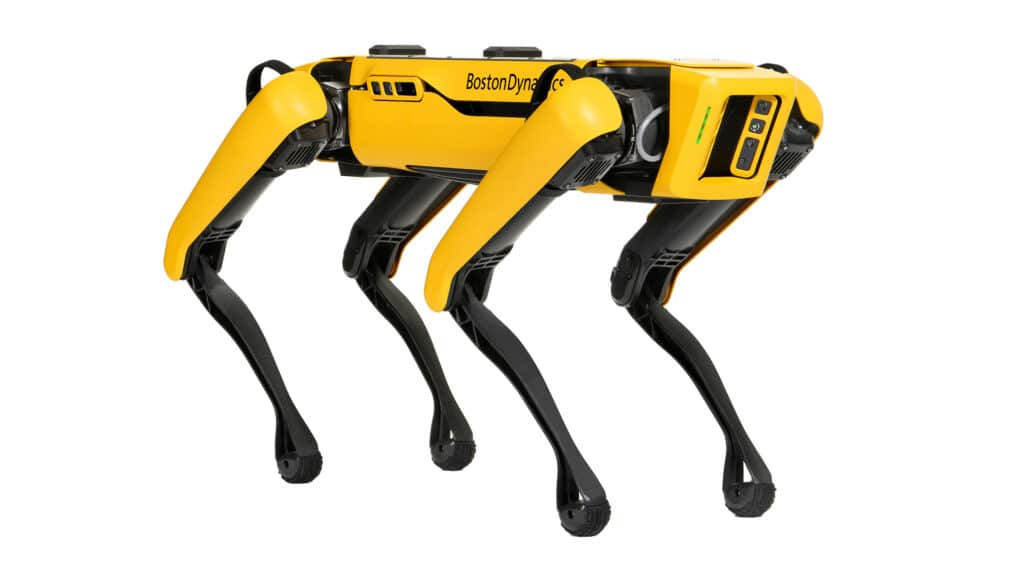
\includegraphics[height=4.2cm]{images/spot_main.jpg}
  \caption{Boston Dynamics Spot}
\endminipage\hfill
\minipage{0.48\textwidth}
  \centering
  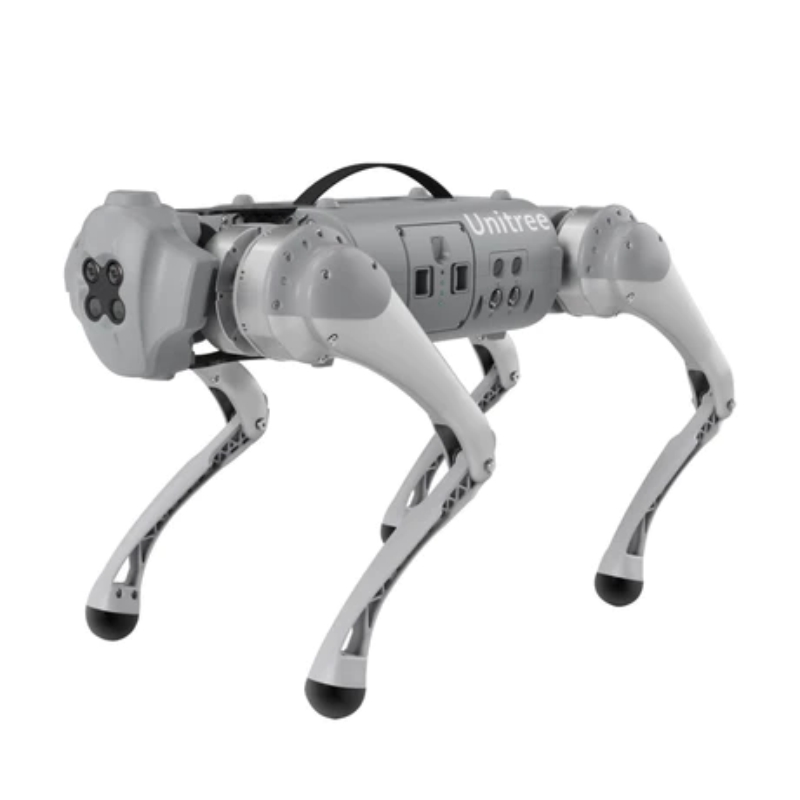
\includegraphics[height=4.2cm]{images/unitree_go1_main.jpg}
  \caption{Unitree Go1}
\endminipage
\end{figure}

\begin{figure}[htbp]
\centering
\minipage{0.48\textwidth}
  \centering
  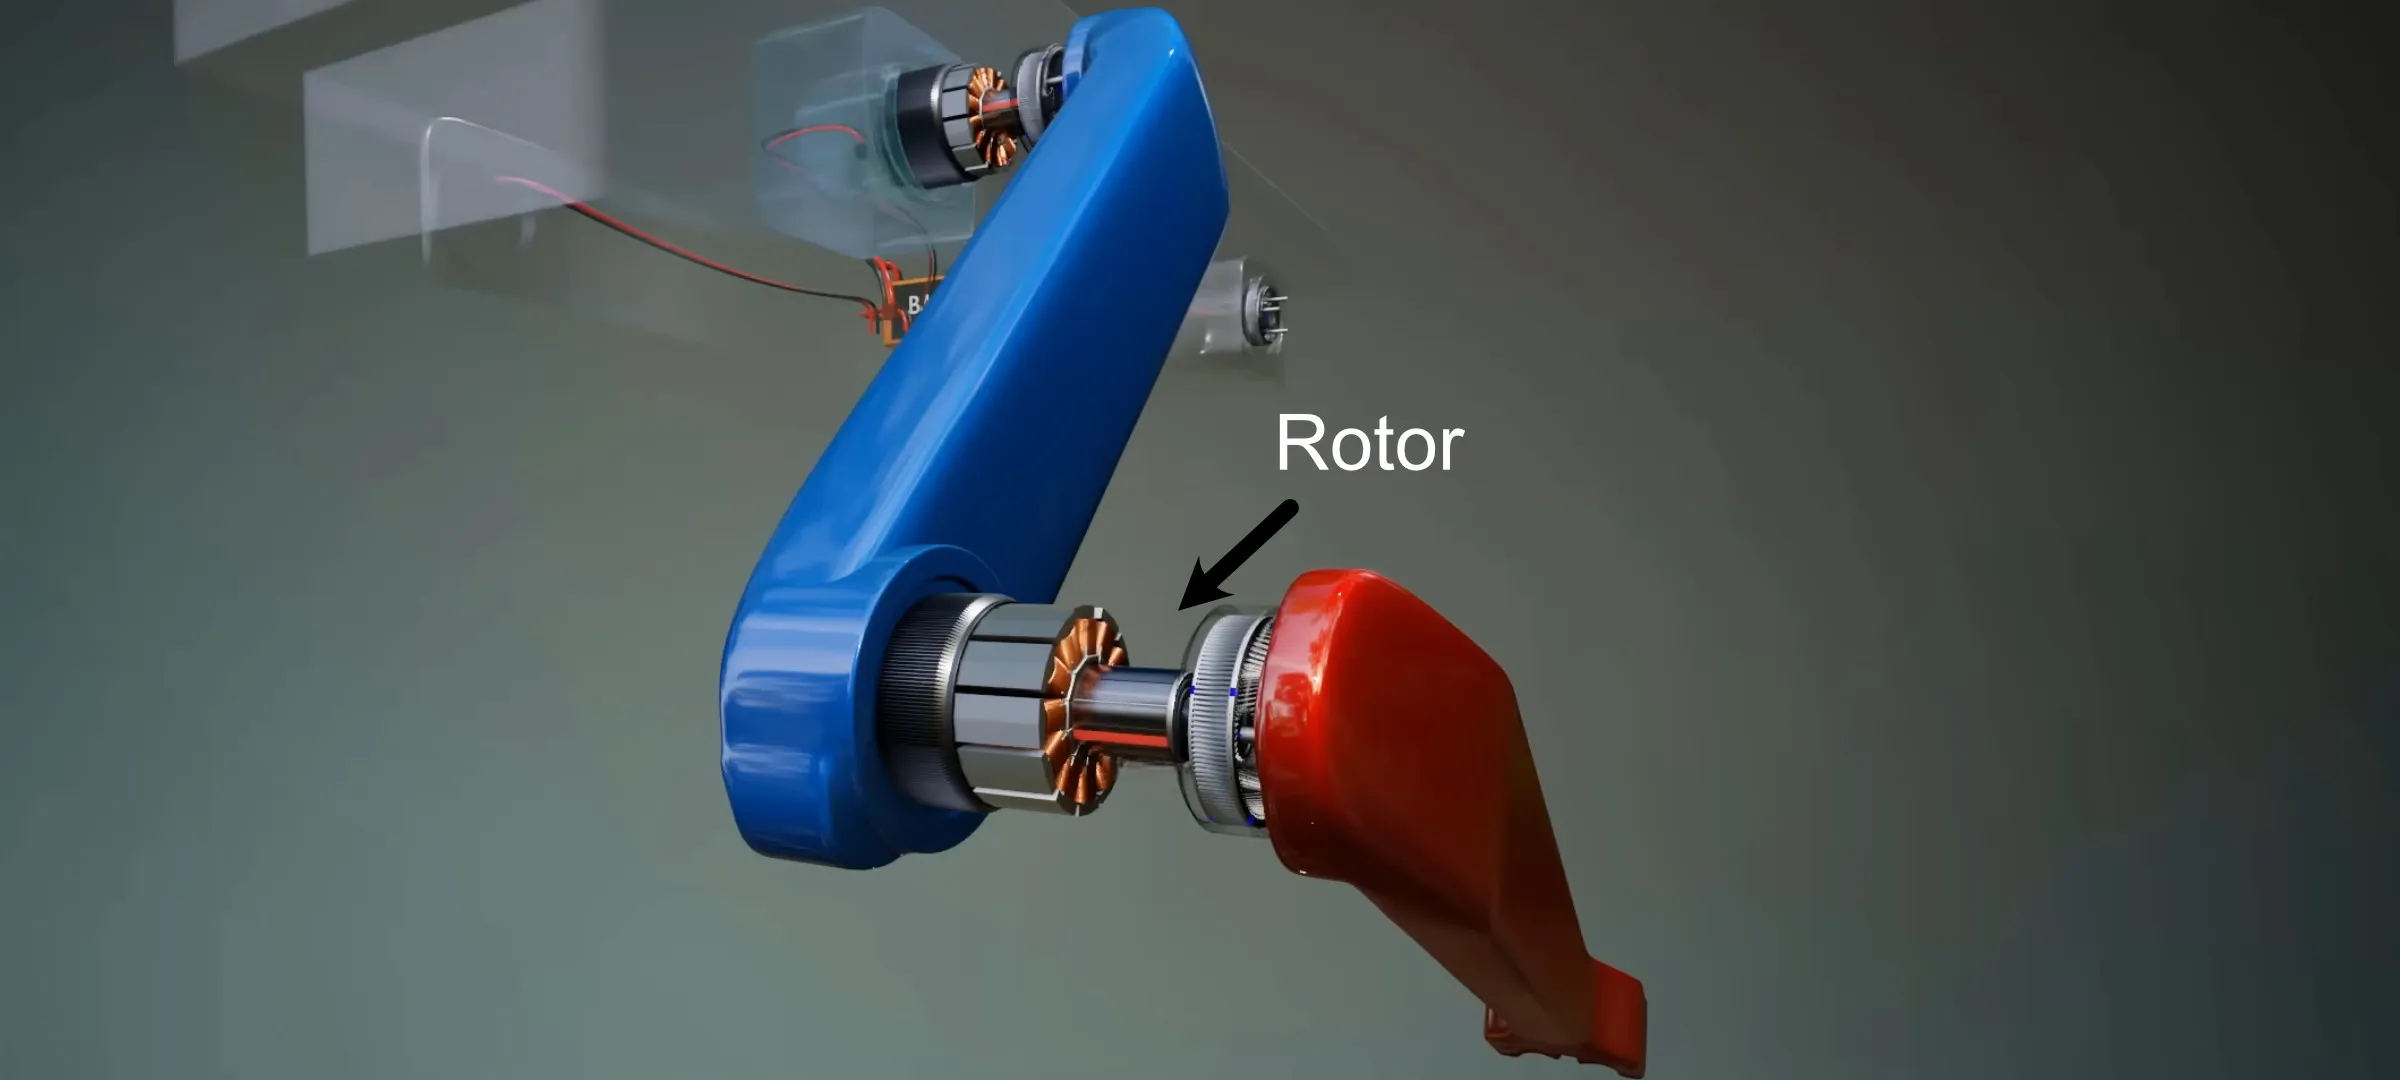
\includegraphics[height=3.4cm]{images/spot_leg.png}
  \caption{Γραμμικός ενεργοποιητής (ball-screw) στο γόνατο του Spot}
\endminipage\hfill
\minipage{0.48\textwidth}
  \centering
  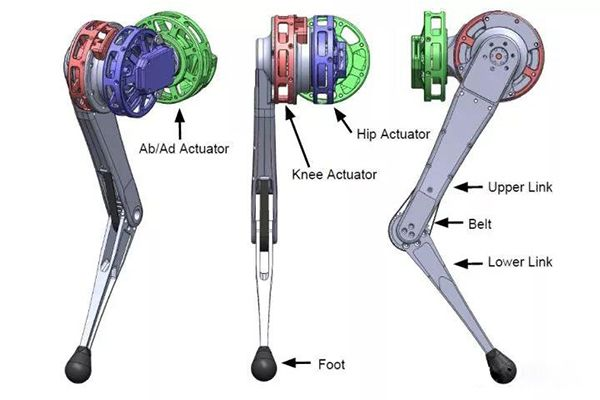
\includegraphics[height=3.4cm]{images/proximal_actuation_leg.jpg}
  \caption{Proximal actuation στον ώμο (φιλοσοφία Unitree/MIT Cheetah)}
\endminipage
\end{figure}

\subsection{Ερευνητικές Πλατφόρμες}
Η σειρά τετράποδων ρομπότ Cheetah του MIT, και πιο συγκεκριμένα τα MIT Cheetah 3
και Mini Cheetah, αποτελούν από τις πιο σύγχρονες και προηγμένες ερευνητικές
πλατφόρμες του πανεπιστημίου. Χρησιμοποιούν κινητήρες υψηλής πυκνότητας ροπής
(high torque density electric motors) με backdriveable μονοβάθμιους πλανητικούς
μειωτήρες (single-stage planetary gear reductions), πόδια χαμηλής αδράνειας, και
ανιχνεύουν την επαφή με το έδαφος μέσω ιδιοδεκτικότητας (proprioception), χωρίς
αισθητήρες δύναμης ή ροπής. Το Cheetah 2 σχεδιάστηκε για γρήγορη κίνηση μόνο στο
οβελιαίο επίπεδο (sagittal plane), καθώς τα πόδια του δεν είχαν δυνατότητα
προσαγωγής/απαγωγής (abduction/adduction). Το Cheetah 3 διόρθωσε αυτόν τον
περιορισμό, προσφέροντας με τους ίδιους κινητήρες πλήρη τρισδιάστατο έλεγχο της
κίνησης \cite{hyun_high_2014,bledt_mit_2018}. Το Mini Cheetah, με τη σειρά του,
έχει τη δυνατότητα εκτέλεσης backflip (πλήρους περιστροφής 360°). Οι αλγόριθμοι
που το καθιστούν αυτό δυνατό βασίζονται σε μοντέλο προβλεπτικού ελέγχου (Model
Predictive Control, MPC), ενώ ο συγχρονισμός της βάδισης στηρίζεται στον
ιδιοδεκτικό εντοπισμό επαφής του ποδιού με το έδαφος και σε μία γεννήτρια
σήματος πριονωτής κυματομορφής (sawtooth waveform generator)
\cite{kim_highly_2019}.

Το ANYmal, αναπτυγμένο στο ETH Zurich, διαθέτει τρεις ενεργοποιούμενες αρθρώσεις
ανά πόδι και σημειακά πέλματα (point feet). Με μήκος συνδέσμου περίπου 250 mm
για μηρό και κνήμη, και συνολικό βάρος λίγο κάτω από 30 kg, θυμίζει σκύλο
μεσαίου μεγέθους. Για τον ελαφρύ αυτόν σχεδιασμό, το κύριο σώμα και τα τμήματα
των ποδιών είναι κατασκευασμένα από αλουμίνιο και ανθρακόνημα (carbon fiber). Οι
ενσωματωμένες μπαταρίες, χωρητικότητας περίπου 650 Wh και βάρους 3 kg, παρέχουν
αυτόνομη λειτουργία άνω των 2 ωρών. Ένα προστατευτικό πλαίσιο με μαξιλαράκια στα
πόδια προστατεύει το σύστημα από ζημιά σε περίπτωση πτώσης και διευκολύνει τη
μεταφορά και την ανάπτυξή του στο πεδίο. Για την αντίληψη του περιβάλλοντος,
χρησιμοποιούνται αισθητήρες Optoforce ως απτικά πέλματα, καθώς και
περιστρεφόμενοι αισθητήρες LiDAR τύπου Hokuyo UTM-30LX για τρισδιάστατη
αντίληψη. Το ANYmal διαθέτει επιπλέον μια αρθρωτή (modular) κεφαλή τύπου
pan-tilt με μεταβλητό φορτίο αισθητήρων ανάλογα με την αποστολή· για παράδειγμα,
στη διάταξη για την πρόκληση ARGOS, η κεφαλή περιελάμβανε οπτικό ζουμ και
θερμική κάμερα για οπτική επιθεώρηση, αισθητήρα ανίχνευσης αερίων, μικρόφωνα για
αναγνώριση ήχου, καθώς και τεχνητό φωτισμό \cite{hutter_anymal_2016}.

\begin{figure}[htbp]
\centering
\minipage{0.32\textwidth}
  \centering
  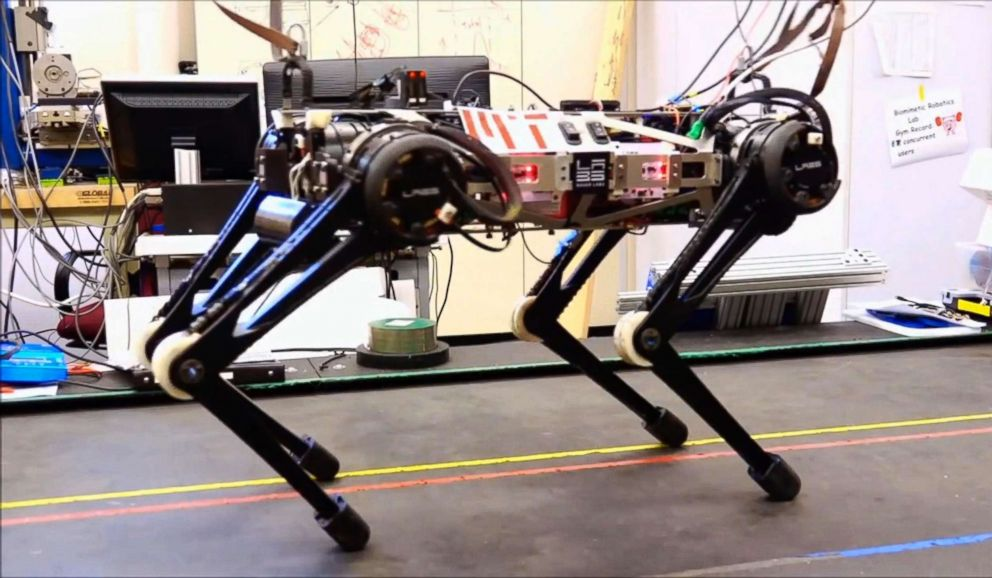
\includegraphics[height=2.9cm]{images/mit_cheetah_3_main.jpg}
  \caption{MIT Cheetah 3}
\endminipage\hfill
\minipage{0.32\textwidth}
  \centering
  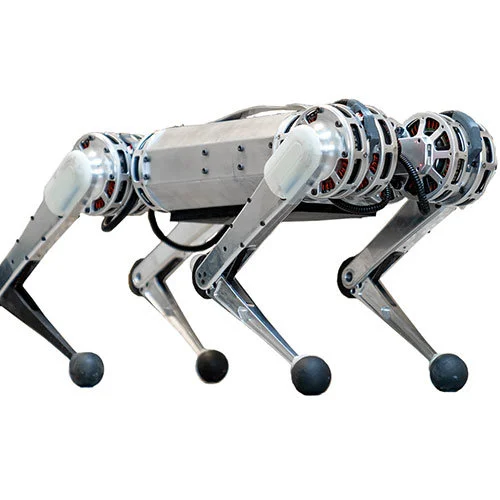
\includegraphics[height=2.9cm]{images/mini_cheetah_main.png}
  \caption{Mini Cheetah}
\endminipage\hfill
\minipage{0.32\textwidth}%
  \centering
  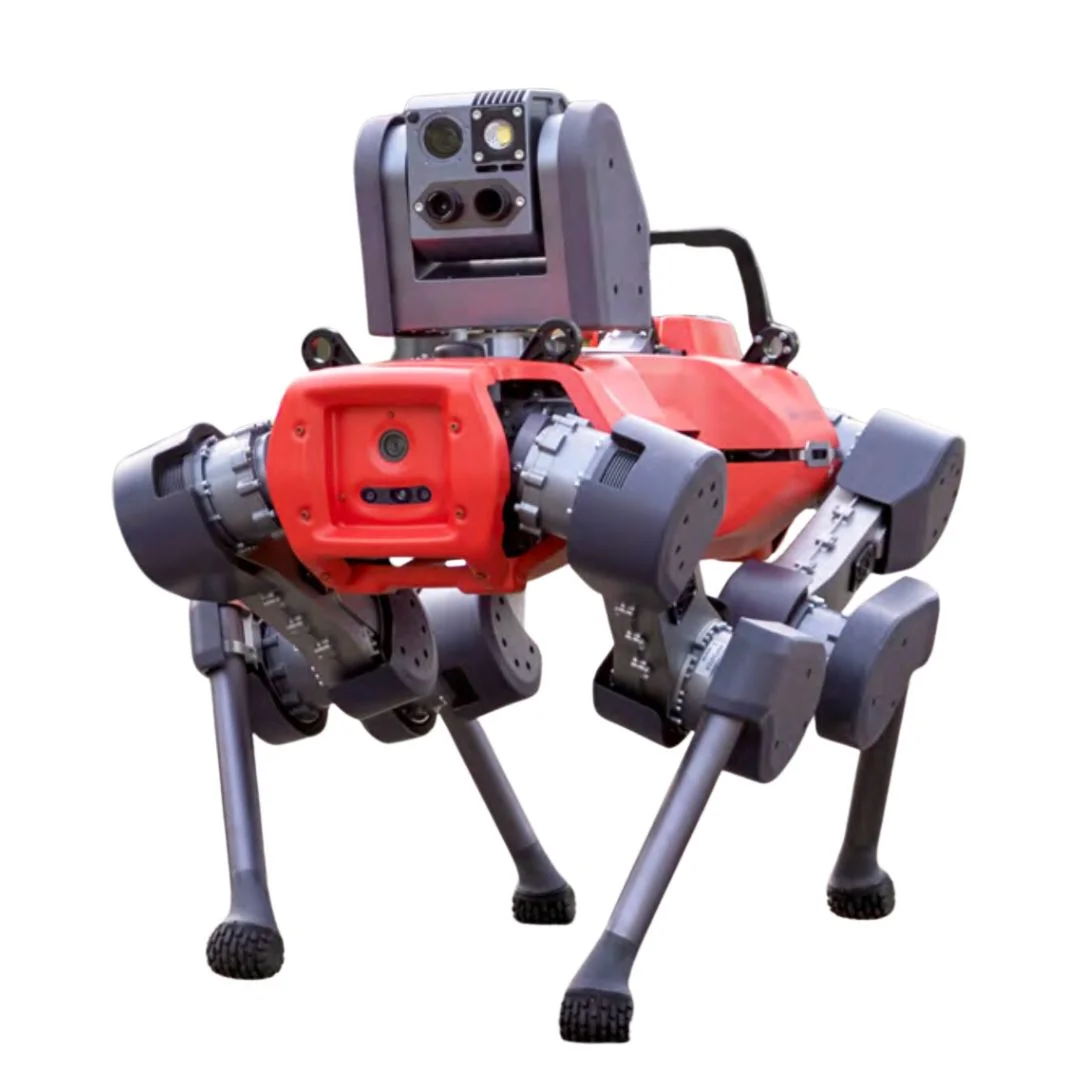
\includegraphics[height=2.9cm]{images/anymal_main.png}
  \caption{ANYmal}
\endminipage
\end{figure}

Κοινό σημείο και των δύο πλατφορμών είναι η χρήση ακριβών ενεργοποιητών ελέγχου
ροπής, γεγονός που αποτελεί χρήσιμη αντίθεση με τους σερβοκινητήρες θέσης που
χρησιμοποιεί η παρούσα εργασία.

\begin{table}[htbp]
    \centering
    \small
    \begin{tabular}{@{}p{2.3cm} p{1.8cm} p{3.0cm} p{1.3cm} p{3.0cm} p{2.0cm}@{}}
        \toprule
        Πλατφόρμα & Κόστος & Ενεργοποιητές άκρου & DOF/πόδι & Αισθητήρες & Ανάδραση \\
        \midrule
        Boston Dynamics Spot &
        \textbullet~Υψηλό\newline\textbullet~Εμπορικό\newline\textbullet~Βιομηχανικό \cite{bostondynamics_spot} &
        \textbullet~Harmonic reducers (ώμος)\newline\textbullet~Ball-screw (γόνατο) \cite{chia_boston_2025,bostondynamics_aboutspot_docs} &
        3 \cite{bostondynamics_aboutspot_docs} &
        \textbullet~Στερεοσκοπικές κάμερες\newline\textbullet~4D LiDAR\newline\textbullet~IMU \cite{bostondynamics_aboutspot_docs,bostondynamics_spot} &
        \textbullet~Torque control \cite{bostondynamics_aboutspot_docs} \\
        \midrule
        Unitree (Go1/Go2) &
        \textbullet~Χαμηλότερο από Spot \cite{unitree_website} &
        \textbullet~Proximal actuation (όλοι στον ώμο) \cite{hyun_high_2014,bledt_mit_2018,ifixit_unitree_go2} &
        3 \cite{ifixit_unitree_go2} &
        \textbullet~4D LiDAR\newline\textbullet~Κάμερες βάθους\newline\textbullet~IMU \cite{ifixit_unitree_go2} &
        \textbullet~Torque control \cite{ifixit_unitree_go2} \\
        \midrule
        MIT Cheetah 3 / Mini Cheetah &
        \textbullet~Ερευνητικό\newline\textbullet~Custom ενεργοποιητές \cite{hyun_high_2014,bledt_mit_2018,kim_highly_2019} &
        \textbullet~Planetary μειωτήρες, backdriveable\newline\textbullet~Proximal actuation \cite{hyun_high_2014,bledt_mit_2018} &
        3 \cite{bledt_mit_2018} &
        \textbullet~Proprioception (ρεύμα κινητήρα)\newline\textbullet~Χωρίς αισθ. δύναμης/ροπής \cite{hyun_high_2014,kim_highly_2019} &
        \textbullet~Torque control \cite{bledt_mit_2018,kim_highly_2019} \\
        \midrule
        ANYmal &
        \textbullet~Ερευνητικό\newline\textbullet~Βιομηχανικό\newline\textbullet~Υψηλό κόστος \cite{hutter_anymal_2016} &
        \textbullet~3 αρθρώσεις/πόδι\newline\textbullet~Σημειακά πέλματα \cite{hutter_anymal_2016} &
        3 \cite{hutter_anymal_2016} &
        \textbullet~Optoforce πέλματα\newline\textbullet~LiDAR Hokuyo \cite{hutter_anymal_2016} &
        \textbullet~Torque control \cite{hutter_anymal_2016} \\
        \midrule
        SpotMicro (και παράγωγα) &
        \textbullet~Χαμηλό\newline\textbullet~Ερασιτεχνικό/DIY \cite{kim_spotmicro_2019,spotmicroai_project} &
        \textbullet~Σερβοκινητήρες θέσης\newline\textbullet~Τυπωμένος σκελετός \cite{kim_spotmicro_2019,taibo_spotmicro_2020} &
        3 \cite{kim_spotmicro_2019} &
        \textbullet~Μόνο IMU\newline\textbullet~Προαιρετικός υπερηχητικός \cite{kim_spotmicro_2019} &
        \textbullet~Position control\newline\textbullet~Χωρίς encoders \cite{kim_spotmicro_2019} \\
        \bottomrule
    \end{tabular}
    \caption{Συγκριτικός πίνακας πλατφορμών τετράποδων ρομπότ (Spot, Unitree, MIT
Cheetah, ANYmal, SpotMicro): κόστος, τύπος ενεργοποιητών, DOF ανά πόδι,
αισθητήρες, είδος ανάδρασης}
    \label{tab:platform-comparison}
\end{table}

\subsection{Πλατφόρμες Ανοιχτού Κώδικα}
Η πιο δημοφιλής πλατφόρμα ανοιχτού κώδικα είναι το SpotMicro από τον Deok-yeon
Kim, εμπνευσμένο από το SpotMini της Boston Dynamics. Είναι τυπωμένο με
τρισδιάστατη εκτύπωση (3D printing), με υλικά τύπου PLA για τον σκελετό και TPU
για τις πατούσες. Χρησιμοποιεί προσβάσιμους μικροελεγκτές, όπως τον Arduino
Mega, και σερβοκινητήρες θέσης. Το αρχικό σχέδιο είχε τη δυνατότητα προσθήκης
αισθητήρα υπερήχων (ultrasonic sensor) για χαρτογράφηση και αποφυγή εμποδίων
\cite{kim_spotmicro_2019}.

Με αφορμή αυτή τη συνεισφορά του Deok-yeon Kim, δημιουργήθηκε η κοινότητα
SpotMicroAI και προέκυψαν διάφορες εκδοχές της πλατφόρμας SpotMicro. Πάνω σε
αυτή τη βάση στηρίχθηκε και το ρομπότ που ανέπτυξαν προηγούμενοι φοιτητές του
τμήματος \cite{tsiatsianas_quadruped_2024}, το οποίο αποτελεί το σημείο
εκκίνησης της παρούσας εργασίας. Η παρούσα εργασία βασίζεται συγκεκριμένα στο
SpotMicro v2 \cite{spotmicroai_project,taibo_spotmicro_2020}.

Μια πολύ ολοκληρωμένη πλατφόρμα που βελτίωσε αισθητά τον μηχανολογικό σχεδιασμό
είναι η SpotMiniMini, η οποία χρησιμοποιεί τη λογική των τριών κινητήρων στον
ώμο, βελτίωσε τον συγχρονισμό της βάδισης με καμπύλες Bezier και υλοποίησε
ενισχυτική μάθηση για βάδιση σε δύσβατο έδαφος \cite{spotminimini2020github}. Η
λογική αυτή, με όλους τους κινητήρες συγκεντρωμένους στον ώμο για μειωμένη
περιστροφική αδράνεια, αντλεί απευθείας από τη φιλοσοφία σχεδιασμού του MIT
Cheetah και της Unitree που παρουσιάστηκε στην προηγούμενη ενότητα, σε
πλατφόρμα όμως δύο έως τριών τάξεων μεγέθους φθηνότερη.

Το τίμημα αυτής της μείωσης κόστους είναι το είδος της διαθέσιμης ανάδρασης: το
SpotMicro και οι παράγωγές του πλατφόρμες χρησιμοποιούν
σερβοκινητήρες θέσης, χωρίς encoders ή αισθητήρες δύναμης/ροπής στις
αρθρώσεις· η μοναδική διαθέσιμη ανάδραση προέρχεται από τον αδρανειακό
αισθητήρα (IMU) του ρομπότ. Η απουσία άμεσης μέτρησης δύναμης/ροπής αποτελεί
τον κεντρικό περιορισμό που καλείται να αντισταθμίσει ο αλγόριθμος
σταθεροποίησης της παρούσας εργασίας (ενότητα~\ref{sec:stabilization}).

Για την παρούσα εργασία χρησιμοποιήθηκε το σχέδιο SpotMicro v2, με μικρές
σχεδιαστικές αλλαγές στην πλάκα βάσης (baseplate) ώστε να προσαρμοστεί στον
επιλεγμένο εξοπλισμό (hardware) — βλ. Κεφάλαιο~\ref{ch:hardware}
\cite{taibo_spotmicro_2020}.

\section{Σχεδιασμός Βάδισης και Τροχιών Άκρου}
Παρατηρώντας την κίνηση των ζώων, διαπιστώνεται ότι κάθε είδος βαδίσματος
(gait) αποτελεί συνδυασμό δύο φάσεων βάδισης:
τη φάση στήριξης (stance), στην οποία το πόδι είναι σε επαφή με το έδαφος
και δίνει ώθηση στο ρομπότ προς την κατεύθυνση κίνησης, και τη φάση αιώρησης
(swing), στην οποία
το πόδι εκτελεί μια τροχιά εναέρια μέχρι το επόμενο σημείο στήριξης. Η
ονομασία των δύο φάσεων δεν είναι ενιαία στη βιβλιογραφία: σε ορισμένες
εργασίες η στήριξη αναφέρεται ως φάση ώθησης (thrust phase) και η αιώρηση ως
φάση πτήσης (flight phase) \cite{lee_turning_2014}, ενώ σε άλλες ως φάση
υποστήριξης (support phase) και φάση αιώρησης (swing phase) αντίστοιχα
\cite{liu_turning_2017}. Στην παρούσα εργασία χρησιμοποιούνται σε όλο το κείμενο
οι όροι στήριξη (stance) και αιώρηση (swing). Ανάλογα με τη διάρκεια
και τον συγχρονισμό των δύο
αυτών φάσεων, προκύπτουν διαφορετικά είδη βαδίσματος, όπως trot, walk, bound,
gallop και pace \cite{silva_review_2026}.

\subsection{Τύποι Βάδισης και Φάσεις Swing/Stance}
\label{subsec:gait-phases}
Ο όρος βάδισμα (gait) αναφέρεται σε ένα μοτίβο διακριτών τοποθετήσεων των
ποδιών, το οποίο εκτελείται με συγκεκριμένη ακολουθία. Τα τετράποδα ρομπότ
διαθέτουν δύο βασικές κατηγορίες βαδισμάτων. Τα στατικά βαδίσματα (static
gaits), όπως το crawl και το wave, χαρακτηρίζονται από το γεγονός ότι η
κατακόρυφη προβολή του κέντρου βάρους παραμένει πάντα εντός του πολυγώνου
στήριξης που σχηματίζουν τα πόδια σε επαφή με το έδαφος. Αντίθετα, στα
δυναμικά βαδίσματα (dynamic gaits), όπως το trot, το pace και το gallop, η
κατακόρυφη προβολή του κέντρου βάρους δεν είναι απαραίτητο να παραμένει εντός
του πολυγώνου στήριξης, εφόσον διατηρείται η δυναμική ευστάθεια
\cite{hu_trotting_2011,raibert_legged_1986,silva_review_2026}.

Το βάδισμα trot επιλέχθηκε και για την παρούσα εργασία, λόγω της
παρατηρούμενης ενεργειακής του αποδοτικότητας σε ευρύ φάσμα ταχυτήτων κίνησης,
καθώς και της ευρείας χρήσης του στη φύση. Πρόκειται για συμμετρικό βάδισμα,
κατά το οποίο το διαγώνιο ζεύγος εμπρόσθιου και οπίσθιου άκρου κινείται σε
συγχρονισμό, ιδανικά με ταυτόχρονη επαφή και αποκόλληση από το έδαφος. Ακόμη
και όταν αυξάνεται η ταχύτητα βάδισης και μειώνεται αντίστοιχα η διάρκεια της
διαγώνιας στήριξης, το εμπρόσθιο ή το οπίσθιο πόδι που
παραμένει σε επαφή με το έδαφος στηρίζει το σώμα, χωρίς το βάδισμα trot να
οδηγεί σε ανατροπή. Για τον λόγο αυτό, το trot θεωρείται πιο σταθερό βάδισμα
\cite{hu_trotting_2011,mori_study_2022}. Στο Σχήμα~\ref{fig:gait-diagram-types}
παρουσιάζονται τα διάφορα είδη βαδίσματος, με το duty factor κάθε ποδιού,
δηλαδή το ποσοστό του κύκλου βάδισης κατά το οποίο το πόδι βρίσκεται σε φάση
στήριξης (stance) \cite{silva_review_2026}.

\begin{figure}[htbp]
    \centering
    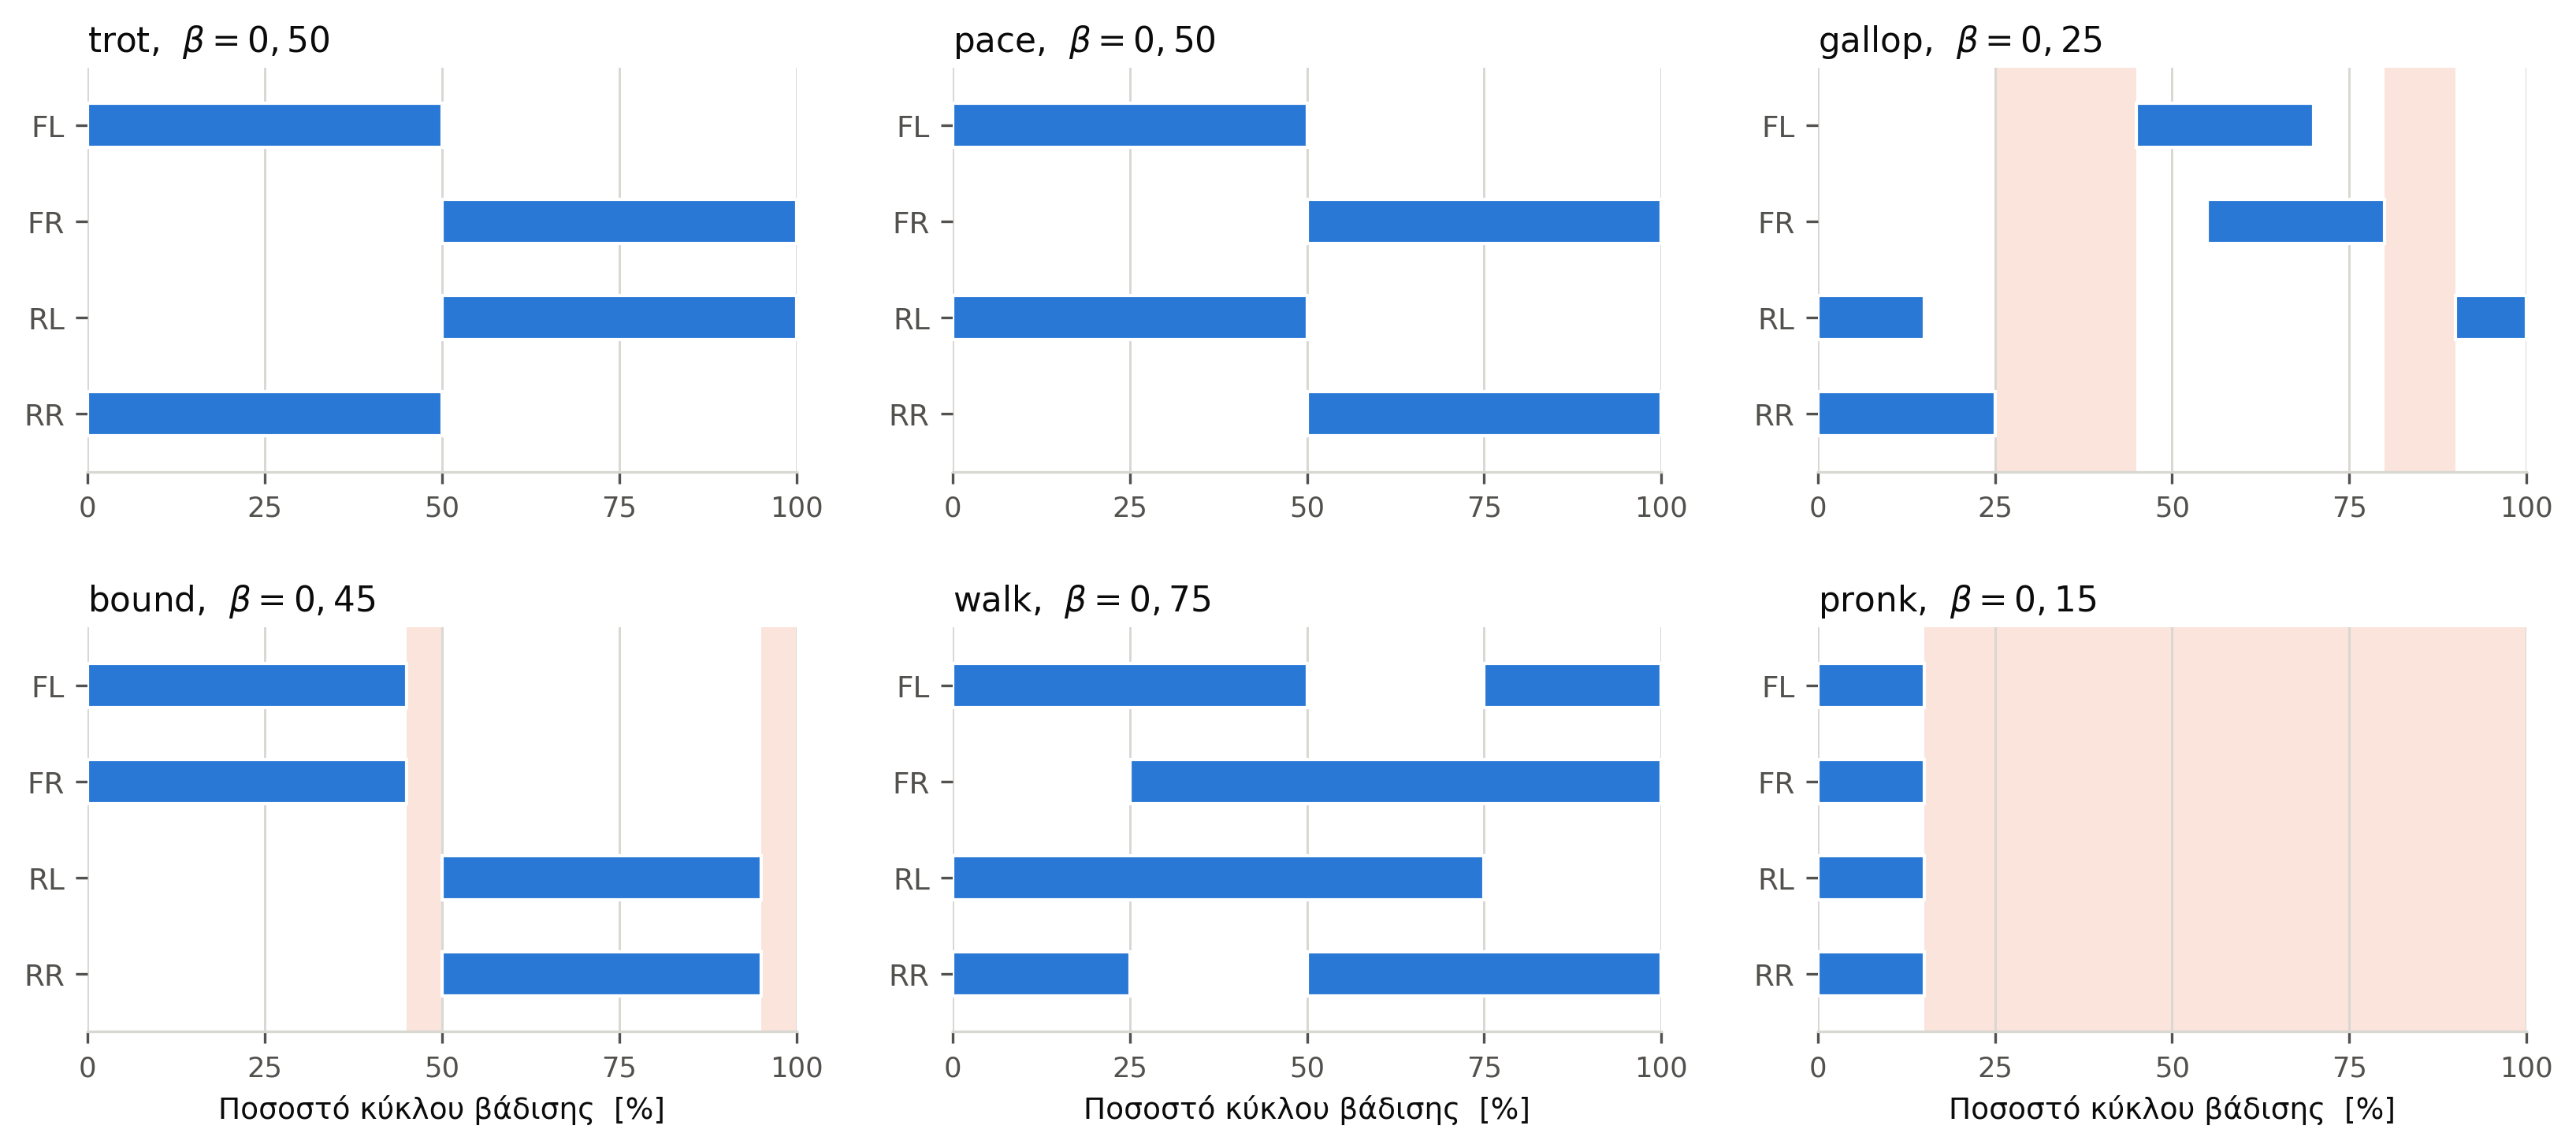
\includegraphics[width=\textwidth]{images/gait_diagrams.png}
    \caption[Διαγράμματα φάσεων βαδίσματος]{Διαγράμματα φάσεων βαδίσματος (gait
    diagrams) για trot, pace, gallop, bound, walk και pronk. Οι γεμάτες
    περιοχές αντιστοιχούν σε φάση στήριξης και ο συντελεστής πλήρωσης $\beta$
    δίνει το ποσοστό του κύκλου κατά το οποίο κάθε πόδι βρίσκεται σε επαφή με
    το έδαφος. Οι σκιασμένες κατακόρυφες λωρίδες σημειώνουν τις φάσεις πτήσης,
    κατά τις οποίες κανένα πόδι δεν είναι σε επαφή}
    \label{fig:gait-diagram-types}
\end{figure}

\begin{table}[htbp]
    \centering
    \small
    \begin{tabular}{@{}l c p{5.7cm} p{3.3cm}@{}}
        \toprule
        Είδος βάδισης & Duty factor & Ακολουθία πατήματος ποδιού & Τυπική ταχύτητα \\
        \midrule
        trot & 50\% & FR+RL $\rightarrow$ FL+RR (διαγώνια εναλλασσόμενα ζεύγη) & Μεσαία ταχύτητα \\
        pace & 50\% & FR+RR $\rightarrow$ FL+RL (πλευρικά εναλλασσόμενα ζεύγη) & Μεσαία ταχύτητα \\
        gallop & 20--30\% & RR $\rightarrow$ RL $\rightarrow$ FR $\rightarrow$ FL (διαδοχικό, με φάση αιώρησης/πτήσης) & Μέγιστη ταχύτητα \\
        bound & 40--50\% & RR+RL $\rightarrow$ FR+FL (πίσω ζεύγος, μετά εμπρός ζεύγος) & Υψηλή ταχύτητα \\
        walk & 70--80\% & RL $\rightarrow$ FL $\rightarrow$ RR $\rightarrow$ FR (διαδοχικό, μετατόπιση 25\% ανά πόδι) & Χαμηλή ταχύτητα (στατικά ευσταθές βάδισμα) \\
        pronk & 10--20\% & FL+FR+RL+RR ταυτόχρονα (πλήρως συγχρονισμένο) & Χαμηλή ταχύτητα μετατόπισης / υψηλή κατακόρυφη ώθηση \\
        \bottomrule
    \end{tabular}
    \caption{Τύποι βαδίσματος: duty factor, ακολουθία πατήματος και τυπική
    ταχύτητα}
    \label{tab:gait-types}
\end{table}

\subsection{Παραμετρικές Τροχιές Στήριξης (Stance): Έλλειψη και Ημίτονο}
Πριν από αναλυτικά βελτιστοποιημένες τροχιές, η βιβλιογραφία χρησιμοποιεί
συχνά απλές παραμετρικές καμπύλες για την περιγραφή της κίνησης του ποδιού.
Κλασικό παράδειγμα αποτελεί η ελλειπτική τροχιά (elliptical trajectory), κατά
την οποία ολόκληρος ο κύκλος βάδισης, δηλαδή η αιώρηση και η στήριξη,
περιγράφεται ως μία ενιαία έλλειψη γύρω από τη νεκρή θέση του ποδιού, με
ελάχιστο αριθμό παραμέτρων: τους δύο ημιάξονες και τη γωνιακή ταχύτητα
διαγραφής της· μια ημι-ελλειψοειδής (half-ellipsoidal) παραλλαγή της έχει
χρησιμοποιηθεί και για τον σχεδιασμό τροχιάς ποδιού σε βάδισμα στροφής
\cite{lee_turning_2014,liu_turning_2017}.

\begin{figure}[htbp]
    \centering
    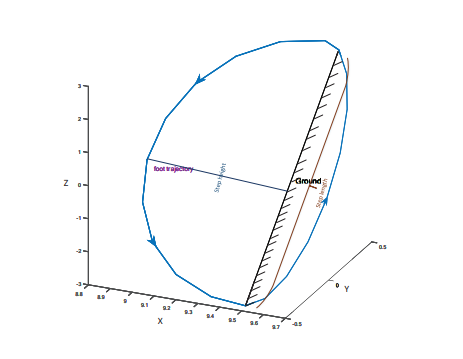
\includegraphics[width=0.5\textwidth]{images/elliptic_curve.png}
    \caption[Ελλειπτική τροχιά ποδιού]{Ελλειπτική τροχιά ποδιού. Πηγή:
\cite{liu_turning_2017}}
    \label{fig:trajectory-elliptic}
\end{figure}

Μια εναλλακτική, πιο ευέλικτη προσέγγιση είναι το ημιτονοειδές
προφίλ (sinusoidal profile), όπου η κατακόρυφη θέση του ποδιού
μεταβάλλεται ως ημίτονο ρυθμιζόμενου πλάτους· η προσέγγιση αυτή χρησιμοποιείται
και στη γεννήτρια τροχιάς σκέλους του MIT Cheetah, η οποία συνδυάζει καμπύλη
Bezier με ημιτονοειδές κύμα ρυθμιζόμενου πλάτους (tunable amplitude sinusoidal
wave) \cite{hyun_high_2014}.

Οι προσεγγίσεις αυτές μοιράζονται κοινά πλεονεκτήματα: απλότητα υλοποίησης
και ελάχιστες παραμέτρους προς ρύθμιση. Το βασικό τους μειονέκτημα είναι ότι η
ταχύτητα του ποδιού δεν μηδενίζεται τη στιγμή της προσγείωσης (touchdown),
γεγονός που προκαλεί κρουστική φόρτιση της άρθρωσης και του εδάφους, αυξημένη
φθορά και απώλεια ενέργειας σε σχέση με τροχιές σχεδιασμένες ειδικά ώστε να
μηδενίζουν την ταχύτητα στα άκρα τους \cite{zeng_leg_2019}.

Στην παρούσα εργασία, η λογική του ημιτονοειδούς προφίλ υιοθετείται
συγκεκριμένα για τη φάση στήριξης (stance): το πόδι ακολουθεί ημιτονοειδή
τροχιά με ρυθμιζόμενο βάθος διείσδυσης $\delta$ ως προς το επίπεδο εδάφους,
ώστε να διατηρείται συνεχής και ελεγχόμενη επαφή καθ' όλη τη διάρκεια της
στήριξης. Την ίδια λογική ημιτονοειδούς στήριξης ακολουθεί και η υλοποίηση
του SpotMiniMini \cite{spotminimini2020github}, ενώ αντίστοιχη αρχή
ρυθμιζόμενου βάθους διείσδυσης ακολουθεί και η γεννήτρια τροχιάς σκέλους του
MIT Cheetah, μέσω του ρυθμιζόμενου πλάτους της ημιτονοειδούς συνιστώσας της
\cite{hyun_high_2014}.

\subsection{Καμπύλες Bezier για την Τροχιά Αιώρησης (Swing)}
\label{subsec:bezier-litreview}
Σε αντίθεση με τη φάση στήριξης, όπου επιδιώκεται συνεχής επαφή με το έδαφος,
η φάση αιώρησης (swing) απαιτεί ταχεία και ομαλή μετακίνηση του ποδιού από το
σημείο απογείωσης (liftoff) στο σημείο προσγείωσης, χωρίς ανεπιθύμητη επαφή με
το έδαφος στο ενδιάμεσο. Για τον σκοπό αυτό, η βιβλιογραφία χρησιμοποιεί
ευρέως καμπύλες Bezier, οι οποίες ορίζονται μέσω πολυωνύμων Bernstein πάνω σε
ένα σύνολο σημείων ελέγχου (control points). Η ίδια η γεννήτρια τροχιάς του
MIT Cheetah βασίζεται σε καμπύλη Bezier για το σκέλος αυτό της κίνησης
\cite{hyun_high_2014}. Το πλεονέκτημα των καμπυλών Bezier έναντι των απλών
παραμετρικών προφίλ είναι ότι τα σημεία ελέγχου προσφέρουν άμεσο έλεγχο όχι
μόνο της θέσης αλλά και της ταχύτητας και της επιτάχυνσης του ποδιού σε κάθε
σημείο της τροχιάς.

Συγκεκριμένα, η επανάληψη (stacking) του ίδιου σημείου ελέγχου στα δύο άκρα
της καμπύλης, στο liftoff και στο touchdown, μηδενίζει την πρώτη και τη
δεύτερη παράγωγο της καμπύλης στα σημεία αυτά, εξασφαλίζοντας μηδενική
ταχύτητα και επιτάχυνση του ποδιού τη στιγμή της απογείωσης και της
προσγείωσης. Η παρούσα εργασία ακολουθεί ακριβώς αυτή την υλοποίηση των 12
σημείων ελέγχου με τριπλή στοίβαξη στα άκρα, όπως ορίζεται στο SpotMiniMini
\cite{spotminimini2020github}, μια προσέγγιση που μειώνει την κρουστική
φόρτιση σε σχέση με τα απλά ημιτονοειδή ή ελλειπτικά προφίλ
\cite{zeng_leg_2019}. Η αρχική τοποθέτηση του ποδιού εντός της τροχιάς
ρυθμίζεται μέσω ενός offset S/6 κατά την προσγείωση, σύμφωνα με τη μέθοδο
βέλτιστης αρχικής θέσης ποδιού για βάδισμα trot \cite{he_optimal_2020}.

\begin{figure}[htbp]
    \centering
    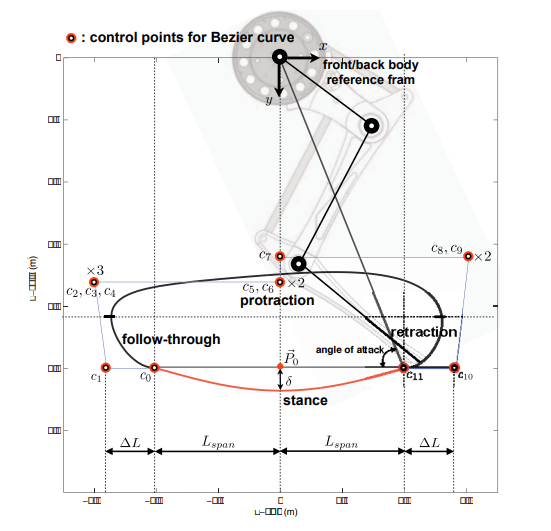
\includegraphics[width=0.6\textwidth]{images/mit_cheetah_3_bezier.png}
    \caption[Σημεία ελέγχου Bezier και ημιτονοειδής τροχιά στήριξης του MIT
Cheetah]{Σημεία ελέγχου Bernstein/Bezier και η προκύπτουσα καμπύλη
τροχιάς αιώρησης (swing), καθώς και η ημιτονοειδής τροχιά στήριξης (stance),
από το MIT Cheetah. Πηγή: \cite{hyun_high_2014}}
    \label{fig:bezier-control-points}
\end{figure}

\subsection{Γεννήτριες Κεντρικών Προτύπων (CPG)}
\label{subsec:cpg}
Οι γεννήτριες κεντρικών προτύπων (Central Pattern Generators, CPGs)
αποτελούν μια εναλλακτική προσέγγιση στον σχεδιασμό τροχιάς, εμπνευσμένη από
έννοιες της βιολογίας και της νευροεπιστήμης. Βιολογικά, αντιστοιχούν σε ένα
σύνολο νευρώνων που βρίσκονται στον νωτιαίο μυελό και είναι υπεύθυνοι για την
παραγωγή ρυθμικών κινητικών εντολών (rhythmic motor commands), χωρίς να
απαιτείται συνεχής εποπτεία από τον εγκέφαλο \cite{silva_review_2026}.

Σε αντίθεση με άλλες μεθόδους ελέγχου, οι CPGs επιτρέπουν άμεσο έλεγχο των
αρθρώσεων του ρομπότ, ή συνολικά κάθε ποδιού, με συγχρονισμό μεταξύ των
άκρων, χωρίς να απαιτούνται σύνθετες υλοποιήσεις μηχανών πεπερασμένων
καταστάσεων (state machines) ή σχεδιαστών τροχιάς (trajectory planners)
\cite{silva_review_2026}.

Μαθηματικά, οι CPGs υλοποιούνται συνήθως ως συστήματα συζευγμένων μη
γραμμικών ταλαντωτών, όπως ο ταλαντωτής Hopf ή ο ταλαντωτής Van der Pol,
έναν ανά πόδι του ρομπότ. Η σύζευξη (coupling) μεταξύ τους καθορίζει τη
σχετική φάση των άκρων και, συνεπώς, τον τύπο του βαδίσματος (trot, pace,
bound κ.λπ.), ο οποίος αναδύεται ως ευσταθής κύκλος ισορροπίας (limit cycle)
του συζευγμένου συστήματος, χωρίς να ορίζεται ρητά από τον σχεδιαστή
\cite{silva_review_2026}.

\begin{figure}[htbp]
    \centering
    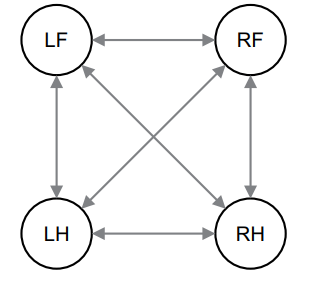
\includegraphics[width=0.5\textwidth]{images/CPG.png}
    \caption[Διάγραμμα σύζευξης τεσσάρων ταλαντωτών CPG για βάδισμα
    trot]{Διάγραμμα σύζευξης τεσσάρων ταλαντωτών CPG, ενός ανά πόδι, για
    την παραγωγή βαδίσματος trot: τα διπλά βέλη δηλώνουν την αμοιβαία
    επιρροή φάσης μεταξύ των ταλαντωτών. Πηγή: \cite{silva_review_2026}}
    \label{fig:cpg-coupling}
\end{figure}

Καθώς ο CPG είναι εγγενώς ανοιχτού βρόχου, έχουν
προταθεί στρατηγικές κλεισίματος του βρόχου ώστε το ρομπότ να γίνεται πιο
προσαρμοστικό· οι Righetti και Ijspeert έκλεισαν τον βρόχο μεταβάλλοντας τις
φάσεις στήριξης και αιώρησης κάθε ποδιού μόνο όταν αυτό έρχεται πραγματικά σε
επαφή ή αποχωρίζεται από το έδαφος, αποφεύγοντας μεταβάσεις σε λάθος στιγμή
που θα μπορούσαν να αποσταθεροποιήσουν το ρομπότ, ιδίως σε ανώμαλο έδαφος
\cite{silva_review_2026}.

Η προσέγγιση της παρούσας εργασίας μπορεί να φανεί συγγενική με τους CPGs,
καθώς και οι δύο παράγουν περιοδική εναλλαγή αιώρησης και στήριξης με
σταθερή σχέση φάσης ανά πόδι. Η θεμελιώδης διαφορά βρίσκεται όμως στην
\emph{πηγή} αυτού του συγχρονισμού. Στους CPGs, η σχέση φάσης μεταξύ των
άκρων αναδύεται από τη δυναμική σύζευξης ενός συστήματος ταλαντωτών· στην
παρούσα εργασία, η σχέση αυτή ανατίθεται ρητά, και η τροχιά κάθε άκρου
υπολογίζεται από κλειστές αναλυτικές εκφράσεις (καμπύλη Bezier για την
αιώρηση, ημίτονο για τη στήριξη) σε συνάρτηση με μια μεταβλητή φάσης που
προωθείται από ρολόι. Πρόκειται δηλαδή για αρχιτεκτονική τύπου μηχανής
πεπερασμένων καταστάσεων με μεταβλητή φάσης (event-based finite state
machine with a phase variable) — την ίδια φιλοσοφία που ακολουθεί και το MIT
Cheetah 3 αντί για CPG \cite{bledt_mit_2018}.

Η υιοθέτηση CPG δεν κρίθηκε απαραίτητη για την παρούσα εργασία, καθώς η ρητή
ανάθεση φάσης και οι κλειστές τροχιές προσφέρουν προβλέψιμη και εύκολα
ρυθμιζόμενη συμπεριφορά για το βάδισμα trot. Η
υλοποίηση CPG παραμένει ωστόσο μια ενδιαφέρουσα κατεύθυνση μελλοντικής
επέκτασης (ενότητα~\ref{sec:future-work}).

\section{Εκτίμηση Καταστάσεως και Σύντηξη Αισθητήρων (State Estimation και Sensor Fusion)}
Για να μπορεί να ελεγχθεί πιο αποδοτικά το ρομπότ, χρειάζεται να είναι
διαθέσιμη η πληροφορία της θέσης στον χώρο αρθρώσεων και στον καρτεσιανό
χώρο, καθώς και ο προσανατολισμός του σώματος, με βάση το επιλεγμένο σύστημα
συντεταγμένων. Έχοντας αυτές τις πληροφορίες σε κάθε χρονική στιγμή,
μπορούμε, με συνδυασμένη εφαρμογή των εξισώσεων του κινηματικού μοντέλου και
δεδομένων από συμπληρωματικούς αισθητήρες (sensor fusion), να επιτύχουμε ένα
ολοκληρωμένο σύστημα ελέγχου κλειστού βρόχου ώστε να ισορροπεί το ρομπότ.

\subsection{Αδρανειακοί Αισθητήρες (IMU)}
Οι αδρανειακοί αισθητήρες είναι ηλεκτρονικές συσκευές που παρέχουν δεδομένα
για μια συγκεκριμένη δύναμη, γωνιακή ταχύτητα και, μερικές φορές, τον
προσανατολισμό ενός σώματος, χρησιμοποιώντας συνδυασμό γυροσκοπίου,
επιταχυνσιόμετρου και μαγνητόμετρου \cite{kivikangas_estimating_2022}. Το
γυροσκόπιο μετρά τη γωνιακή ταχύτητα
σε κάθε άξονα, το επιταχυνσιόμετρο την γραμμική επιτάχυνση σε κάθε άξονα, και
το μαγνητόμετρο μετρά την ένταση και την κατεύθυνση του μαγνητικού πεδίου.
Όταν οι επιμέρους αισθητήρες μετρούν τα παραπάνω δεδομένα σε κάθε άξονα του
χώρου, τότε έχουμε 6-DOF ή 9-DOF IMU \cite{mori_study_2022,prayogo_quadruped_2018}.

Με βάση τα ακατέργαστα δεδομένα που λαμβάνουμε από το γυροσκόπιο, μπορούμε με
ολοκλήρωση των δεδομένων να λάβουμε τον προσανατολισμό του σώματος, και με τα
δεδομένα από το επιταχυνσιόμετρο να λάβουμε τη γραμμική ταχύτητα και τη θέση
του σώματος. Το μαγνητόμετρο, που δεν συμπεριλαμβάνεται πάντα στους
αδρανειακούς αισθητήρες, χρησιμοποιείται ως πυξίδα για να ξέρουμε πού κοιτάει
το ρομπότ. Αυτές οι απλές υπολογιστικές μέθοδοι είναι επιρρεπείς σε
σφάλματα όπως το bias, ο συντελεστής κλίμακας (scale factor) και οι
μαγνητικές παρεμβολές, καθώς πρόκειται για δυναμικό σύστημα του οποίου η
κατάσταση υπολογίζεται μέσω ολοκλήρωσης, αλλοιώνοντας σημαντικά τα δεδομένα
μετά από κάποιο χρονικό διάστημα \cite{kivikangas_estimating_2022}. Ιδανικά,
απαιτείται ο συνδυασμός ενός χαμηλοπερατού φίλτρου (low-pass), που
αφαιρεί τις συνιστώσες υψηλής συχνότητας του θορύβου, με ένα υψιπερατό
φίλτρο (high-pass) πολύ χαμηλής συχνότητας αποκοπής, που αφαιρεί
bias χαμηλής συχνότητας, χωρίς απώλεια χρήσιμης πληροφορίας
από το ίδιο το σήμα \cite{cocoli_comparative_2023}. Για αυτόν τον λόγο,
παρακάτω θα αναλυθούν αλγόριθμοι σύντηξης αισθητήρων, καθώς και φίλτρα που
βοηθούν στην αντιμετώπιση του θορύβου των δεδομένων και αξιοποιούνται
κασκοδικά όπως φαίνεται στο Σχήμα \ref{fig:imu-fusion-block}.

Στην παρούσα εργασία, παρόλο που ο IMU είναι 9-DOF, δεν αξιοποιήθηκε το
μαγνητόμετρο, διότι βρίσκεται τοποθετημένο κοντά σε πολλά ηλεκτρονικά και δεν
μπορεί να παρέχει σωστά και αξιόπιστα δεδομένα.

\begin{figure}[htbp]
    \centering
    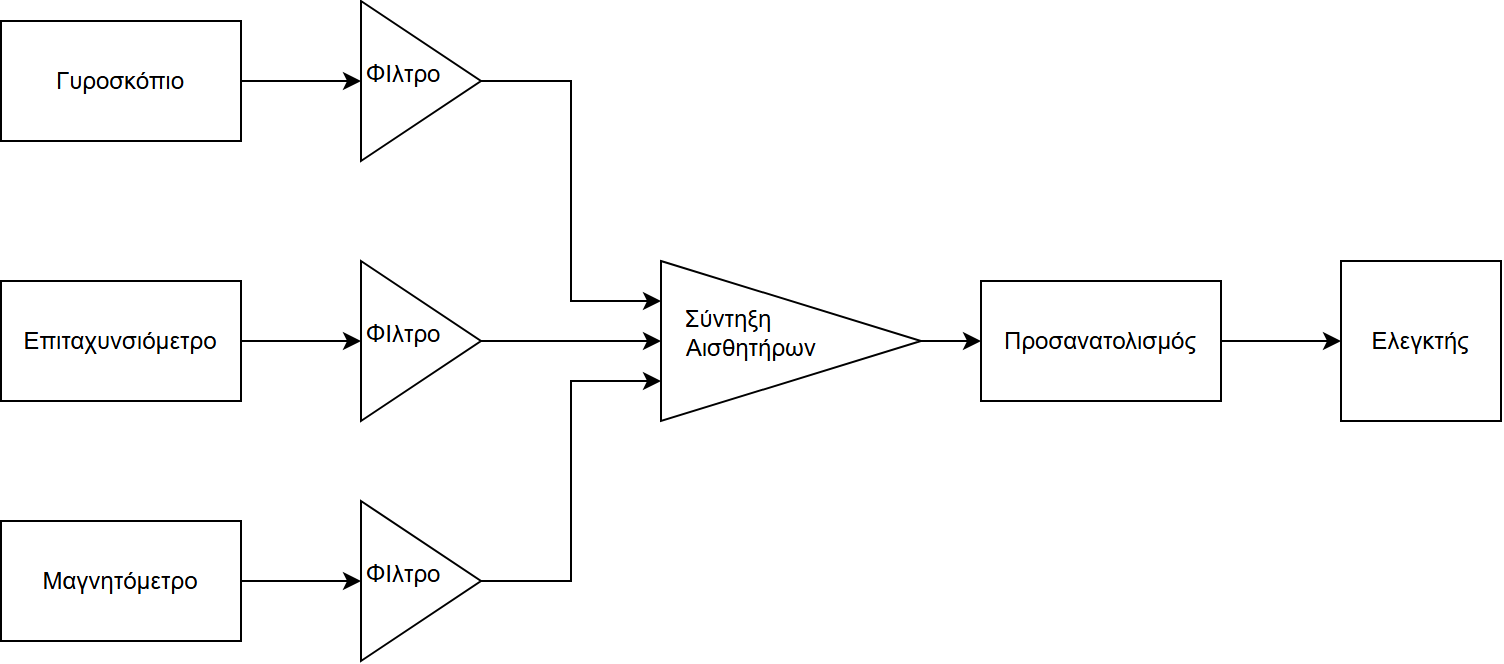
\includegraphics[width=0.85\textwidth]{images/imu_fusion_block.png}
    \caption{Αλυσίδα σύντηξης αισθητήρων IMU: γυροσκόπιο, επιταχυνσιόμετρο
    και μαγνητόμετρο(προαιρετικά) $\rightarrow$ σύντηξη
    αισθητήρων $\rightarrow$ φίλτρο $\rightarrow$ προσανατολισμός $\rightarrow$ ελεγκτής}
    \label{fig:imu-fusion-block}
\end{figure}

\subsection{Εξωτεροδεκτικοί Αισθητήρες: LiDAR και Όραση}
Πέρα από τους αδρανειακούς αισθητήρες, πολλές πλατφόρμες τετράποδων ρομπότ
ενσωματώνουν εξωτεροδεκτικούς αισθητήρες (exteroceptive sensors), όπως LiDAR
και κάμερες βάθους (depth cameras), για την αντίληψη του περιβάλλοντος και
του εδάφους. Χαρακτηριστικό παράδειγμα αποτελεί η σύζευξη LiDAR-IMU σε
αλγορίθμους SLAM (Simultaneous Localization and Mapping), οι οποίοι
επιτρέπουν ταυτόχρονο εντοπισμό και χαρτογράφηση σε ανώμαλο έδαφος
\cite{zhou_tightly-coupled_2024}. Η παρούσα εργασία δεν αξιοποιεί τέτοιους
αισθητήρες, καθώς το αντικείμενό της περιορίζεται στη σταθεροποίηση της
βάδισης σε γνωστό, επίπεδο έδαφος, και όχι στην αυτόνομη πλοήγηση ή
χαρτογράφηση, ζήτημα που ξεπερνά το πλαίσιό της.

\subsection{Ιδιοδεκτική Ανάδραση (Proprioceptive Sensing)}
Μια εναλλακτική μορφή ανάδρασης, που υιοθετείται σε πλατφόρμες όπως το MIT
Cheetah, είναι η ιδιοδεκτική ανάδραση (proprioceptive sensing): αντί για
αισθητήρες δύναμης στα πέλματα, χρησιμοποιούνται backdrivable κινητήρες
χαμηλής σχέσης μετάδοσης, όπου το ίδιο το ρεύμα του κινητήρα λειτουργεί ως
έμμεσος εκτιμητής της δύναμης αντίδρασης εδάφους (proprioceptive impedance
control), επιτρέποντας ανίχνευση της επαφής του ποδιού με το έδαφος χωρίς
εξωτερικό αισθητήρα \cite{hyun_high_2014,lee_hierarchical_2013}. Η προσέγγιση
αυτή προϋποθέτει ειδικά σχεδιασμένους ενεργοποιητές υψηλής διαφάνειας
(transparency) και δεν είναι εφαρμόσιμη στους τυπικούς σερβοκινητήρες θέσης
της παρούσας εργασίας, οι οποίοι δεν παρέχουν πρόσβαση σε μέτρηση ρεύματος ή
ροπής.

\subsection{Αισθητήρες Επαφής στα Άκρα}
Άλλη διαδεδομένη λύση είναι η απευθείας τοποθέτηση αισθητήρων επαφής στα
άκρα, όπως διακόπτες ή αισθητήρες δύναμης/πίεσης στα πέλματα, οι οποίοι
επιτρέπουν άμεση ανίχνευση της φάσης στήριξης και, σε ορισμένες περιπτώσεις,
αναγνώριση του τύπου εδάφους \cite{vangen_terrain_2023}. Σε αντίθεση με αυτές
τις προσεγγίσεις, η παρούσα εργασία χρησιμοποιεί σερβοκινητήρες θέσης χωρίς
encoders ή αισθητήρες επαφής, με τη μοναδική διαθέσιμη ανάδραση να προέρχεται
από το IMU.

\subsection{Αλγόριθμοι Σύντηξης}

Το φίλτρο Kalman παρέχει τη βέλτιστη εκτίμηση της κατάστασης ενός γραμμικού
δυναμικού συστήματος από θορυβώδεις μετρήσεις, υπό την παραδοχή ότι ο θόρυβος
της διαδικασίας και των μετρήσεων ακολουθεί κανονική (Gaussian) κατανομή. Η
λειτουργία του βασίζεται σε δύο επαναλαμβανόμενα βήματα: στο βήμα πρόβλεψης
(prediction), το φίλτρο προβάλλει την κατάσταση και τη συνδιακύμανσή της στην
επόμενη χρονική στιγμή, με βάση ένα μοντέλο μετάβασης κατάστασης· στο βήμα
διόρθωσης (correction), η πρόβλεψη συγκρίνεται με τη νέα μέτρηση, και η
διαφορά τους (καινοτομία ή residual) χρησιμοποιείται για την αναθεώρηση της
εκτίμησης, σταθμισμένη από το κέρδος Kalman (Kalman gain). Το κέρδος αυτό
προσαρμόζεται δυναμικά: όσο μεγαλύτερος ο θόρυβος των μετρήσεων σε σχέση με
την αβεβαιότητα της πρόβλεψης, τόσο μικρότερο το κέρδος, δίνοντας μεγαλύτερη
βαρύτητα στην πρόβλεψη έναντι της μέτρησης, και αντίστροφα \cite{kalman_new_1960}.

Το εκτεταμένο φίλτρο Kalman (Extended Kalman Filter, EKF) επεκτείνει τη
λογική αυτή σε μη γραμμικά συστήματα, όπως ο προσδιορισμός προσανατολισμού
από δεδομένα IMU, γραμμικοποιώντας τις μη γραμμικές συναρτήσεις γύρω από την
τρέχουσα εκτίμηση μέσω πινάκων Ιακωβιανής (Jacobian), αντί των σταθερών
πινάκων μετάβασης του κλασικού φίλτρου. Στην εφαρμογή προσδιορισμού
προσανατολισμού, η κατάσταση αναπαρίσταται συνήθως ως τετραδόνιο
(quaternion), το οποίο αποφεύγει το πρόβλημα του gimbal lock που εμφανίζουν
οι γωνίες Euler. Ο Sabatini προτείνει ένα τετραδονιακό EKF όπου η γωνιακή
ταχύτητα του γυροσκοπίου χρησιμοποιείται στο βήμα πρόβλεψης για την
ολοκλήρωση του τετραδονίου, ενώ οι μετρήσεις επιταχυνσιόμετρου και
μαγνητόμετρου χρησιμοποιούνται στο βήμα διόρθωσης, συγκρίνοντας τις
αναμενόμενες διευθύνσεις βαρύτητας και μαγνητικού πεδίου, στο πλαίσιο
αναφοράς, με τις πραγματικές μετρήσεις· η απόκλιση μεταξύ των δύο τροφοδοτεί
τη διόρθωση του τετραδονίου. Στο μοντέλο του Sabatini, η μεροληψία (bias) του
γυροσκοπίου και οι μαγνητικές διαταραχές μοντελοποιούνται ως επιπλέον
στοιχεία του διανύσματος κατάστασης, ενώ ανάλυση παρατηρησιμότητας
(observability) καθορίζει τις συνθήκες υπό τις οποίες το σύστημα παρέχει
επαρκή πληροφορία για αξιόπιστη εκτίμηση
\cite{sabatini_kalmanfilterbased_2011,garcia_ahrs}.

Το φίλτρο Madgwick αποτελεί μια πολύ πιο πρόσφατη και καινοτόμο εναλλακτική
στα φίλτρα τύπου Kalman, δημοσιευμένη το 2010, σε αντίθεση με το φίλτρο
Kalman του οποίου η θεωρητική βάση χρονολογείται από το 1960. Αντί για
στοχαστική μοντελοποίηση κατάστασης, χρησιμοποιεί μια αναλυτικά παραγόμενη
και βελτιστοποιημένη μέθοδο gradient descent, η οποία υπολογίζει τον
προσανατολισμό που ευθυγραμμίζει καλύτερα τις αναμενόμενες κατευθύνσεις
αναφοράς (βαρύτητα από το επιταχυνσιόμετρο, μαγνητικό πεδίο της Γης από το
μαγνητόμετρο) με τις πραγματικές μετρήσεις, εκφρασμένος ως τετραδόνιο. Το
αποτέλεσμα αυτής της διόρθωσης συνδυάζεται συμπληρωματικά με την ολοκλήρωση
της γωνιακής ταχύτητας του γυροσκοπίου, ώστε να αντισταθμίζεται η ολίσθηση
της ολοκλήρωσης χωρίς να επιτρέπεται ο θόρυβος του επιταχυνσιόμετρου να
αποσταθεροποιήσει την εκτίμηση. Χαρακτηριστικό της καινοτομίας του είναι ότι
απαιτεί μόλις 109 (IMU) ή 277 (MARG) πράξεις ανά ενημέρωση, παραμένει
αποτελεσματικό ακόμη και σε πολύ χαμηλούς ρυθμούς δειγματοληψίας (π.χ. 10
Hz), και διαθέτει μόλις μία ή δύο ρυθμιζόμενες παραμέτρους. Στην αρχική του
αξιολόγηση, ο Madgwick το συνέκρινε με έναν καθιερωμένο αλγόριθμο βασισμένο
σε Kalman και έδειξε ότι το δικό του φίλτρο πετυχαίνει μεγαλύτερη ακρίβεια
(σφάλμα RMS {\textless}0.6° σε στατικές και {\textless}0.8° σε δυναμικές
συνθήκες), παρά τον πολύ μικρότερο υπολογιστικό φόρτο του
\cite{madgwick_efficient_2010}.

Ο κύριος λόγος για τον οποίο επιλέχθηκε το EKF αντί του Madgwick είναι ότι το
δεύτερο παρουσιάζει έντονη ταλάντωση σε κατάσταση ηρεμίας, ενώ σε κατάσταση
κίνησης παρέχει αξιόπιστα δεδομένα, συγκρίσιμα με του EKF. Στη συγκριτική
μελέτη των Çoçoli και Badia, το φαινόμενο αυτό αποδίδεται στην παράμετρο
κέρδους $\beta$ του φίλτρου Madgwick: μια υψηλότερη τιμή του $\beta$
προσφέρει μεγαλύτερο εύρος ζώνης απόκρισης, ώστε το φίλτρο να ακολουθεί
γρήγορες αλλαγές προσανατολισμού το ίδιο γρήγορα με τα υπόλοιπα φίλτρα, με
αντίτιμο την είσοδο περισσότερου θορύβου στην εκτίμηση· στις δικές τους
στατικές δοκιμές, το Madgwick εμφάνισε αισθητά μεγαλύτερες ταλαντώσεις γύρω
από την πραγματική τιμή σε σχέση με τα φίλτρα Kalman και Mahony, ενώ σε
συνθήκες κίνησης η απόδοσή του πλησίαζε αυτή του Kalman
\cite{cocoli_comparative_2023}. Στην πράξη, η ταλάντωση αυτή στην ηρεμία
αποδείχθηκε προβληματική, καθώς ήταν δύσκολο να επιτευχθεί σωστό tuning
ώστε το φίλτρο να συγκλίνει καθώς κινείται το ρομπότ χωρίς απότομες αιχμές
(spikes), οι οποίες, περνώντας στον ελεγκτή, θα μπορούσαν να προκαλέσουν
βλάβη στο ίδιο το ρομπότ. Η επιλογή αυτή συνάδει άλλωστε και με το
συμπέρασμα των Çoçoli και Badia, οι οποίοι προτείνουν το φίλτρο Kalman ως
την προτιμότερη επιλογή όταν η ακρίβεια αποτελεί την κύρια προτεραιότητα και
δεν υπάρχει αυστηρός περιορισμός υπολογιστικών πόρων
\cite{cocoli_comparative_2023}. Η υλοποίηση της παρούσας εργασίας
στηρίχθηκε εκτενώς στη βιβλιοθήκη \texttt{ahrs}, η οποία θα αναλυθεί
παρακάτω \cite{garcia_ahrs}.


\section{Έλεγχος Ευστάθειας Τετράποδων}
Η έρευνα γύρω από αλγορίθμους ελέγχου τετράποδων ρομπότ διεξάγεται
συστηματικά από τη δεκαετία του 1960, με αποτέλεσμα να έχουν διαμορφωθεί
αρκετές κυρίαρχες προσεγγίσεις. Η θεωρία του σημείου μηδενικής ροπής (Zero
Moment Point, ZMP) λαμβάνει υπόψη τις αδρανειακές δυνάμεις που προκύπτουν
κατά την κίνηση του ρομπότ σε στατικό βάδισμα, απαιτεί όμως μεγάλο
υπολογιστικό φόρτο που δυσχεραίνει τη λειτουργία σε πραγματικό χρόνο και δεν
προσαρμόζεται καλά σε ανώμαλο έδαφος. Οι γεννήτριες κεντρικών προτύπων
(Central Pattern Generators, CPG), όπως παρουσιάστηκαν και στην
ενότητα~\ref{subsec:cpg}, μιμούνται νευρωνικά δίκτυα του κεντρικού νευρικού συστήματος, οι
παράμετροί τους όμως είναι σχετικά πολύπλοκες και δύσκολες στη ρύθμιση. Το
μοντέλο του φορτισμένου ανεστραμμένου εκκρεμούς (Spring-Loaded Inverted
Pendulum, SLIP) αποσυνθέτει τον έλεγχο της στάσης του ρομπότ σε επιμέρους
μεγέθη (ύψος αναπήδησης, ταχύτητα προς τα εμπρός, θέση σώματος), ελεγχόμενα
ανεξάρτητα μέσω αναλογικού-διαφορικού (PD) ελεγκτή, με την έννοια του
εικονικού ποδιού (virtual leg) να απλοποιεί τον έλεγχο πολλαπλών ποδιών σε
έλεγχο ενός μόνο. Ο έλεγχος εικονικού μοντέλου (Virtual Model Control, VMC)
επεκτείνει τη λογική αυτή, εστιάζοντας στο κέντρο μάζας του σώματος αντί
στα ίδια τα πόδια, μέσω εικονικών ελατηρίων και αποσβεστήρων· ωστόσο, οι
παράμετροι του ελεγκτή PD που χρησιμοποιεί προσδιορίζονται μόνο εμπειρικά,
είναι ευαίσθητες στις παραμέτρους του μοντέλου, και δύσκολα ρυθμίζονται
\cite{shi_structural_2021}.

Στην παρούσα εργασία επιλέχθηκε ο κλασικός έλεγχος PID αντί για κάποια από
τις παραπάνω προσεγγίσεις, για τρεις κυρίως λόγους. Πρώτον, οι προηγμένες
αυτές μέθοδοι είναι υπερβολικά πολύπλοκες για τις ανάγκες της συγκεκριμένης
εφαρμογής. Δεύτερον, δεν είναι εφαρμόσιμες στο διαθέσιμο υλικό (hardware)
της εργασίας, καθώς προϋποθέτουν έλεγχο δύναμης ή ροπής στις αρθρώσεις, ενώ
οι σερβοκινητήρες θέσης που χρησιμοποιούνται δεν προσφέρουν τέτοια ανάδραση.
Τρίτον, ο ελεγκτής PID είναι αξιόπιστος, υλοποιείται με ελάχιστες γραμμές
κώδικα, και για μια κατασκευή τόσο χαμηλού κόστους όσο η παρούσα, η απόδοσή
του είναι υπεραρκετή.

\subsection{Κλασικός Έλεγχος: PID}
\label{subsec:pid-litreview}
Βάσει της βιβλιογραφίας που αξιοποιήθηκε, παρατηρήθηκε ότι ένας βέλτιστος
τρόπος χρήσης ελεγκτή PID είναι η αντιστάθμιση του ύψους του τελικού άκρου
μέσω σύνδεσής του με τη γωνία που διαβάζει το IMU, μέσω μιας γεωμετρικής
σχέσης που συνδέει τις γωνίες roll/pitch με το πλάτος και το μήκος του
σώματος. Αρχικά εξετάστηκε η απευθείας διόρθωση της γωνίας του σώματος του
ρομπότ, από την οποία, με βάση το κινηματικό μοντέλο, θα προέκυπτε πάλι
αντίστοιχη διόρθωση στο ύψος κάθε άκρου· η προσέγγιση αυτή όμως δεν
αποδείχθηκε τόσο αποτελεσματική. Τόσο ο Mori όσο και ο Prayogo ακολουθούν
την ίδια βασική στρατηγική αντιστάθμισης του ύψους κάθε άκρου με βάση τη
γωνία του IMU, διαφέρουν όμως στην πολυπλοκότητα του ελεγκτή: ο πρώτος
χρησιμοποιεί πλήρη ελεγκτή PID \cite{mori_study_2022}, ενώ ο δεύτερος
επιτυγχάνει ικανοποιητικά αποτελέσματα ακόμη και σε κεκλιμένο έδαφος
χρησιμοποιώντας απλό αναλογικό (P) ελεγκτή, χωρίς την πολυπλοκότητα του
ολοκληρωτικού και διαφορικού όρου \cite{prayogo_quadruped_2018}. Πιο
αναλυτικά η μαθηματική διατύπωση παρουσιάζεται παρακάτω στη μοντελοποίηση.

Η προσέγγιση της παρούσας εργασίας συνδυάζει ουσιαστικά τις δύο αυτές
λογικές: το σφάλμα υπολογίζεται απευθείας πάνω στις γωνίες roll και pitch,
όπως στην αρχική προσέγγιση που εξετάστηκε, χωρίς όμως να τροφοδοτείται στο
κινηματικό μοντέλο ως διόρθωση της στάσης του σώματος. Αντ' αυτού, από τη
διορθωμένη τιμή roll/pitch υπολογίζεται το αντίστοιχο ύψος αντιστάθμισης ανά
πόδι, με τη λογική του Mori και του Prayogo, και το πόδι μετακινείται
απευθείας κατά το ύψος αυτό. Για την αποφυγή φαινομένων ολοκληρωτικής
υπερφόρτωσης (integral
windup) κατά τη διάρκεια παρατεταμένου σφάλματος, όπως σε μια στροφή ή σε
κεκλιμένο έδαφος, ο ολοκληρωτικός όρος του ελεγκτή περιορίζεται εντός ενός
άνω ορίου (anti-windup μέσω κορεσμού), μια κλασική τεχνική που αναλύεται
διεξοδικά στην ανασκόπηση (review) των Caparroz κ.ά. \cite{caparroz_antiwindup_2026}.

\subsection{Ευρετικοί Κανόνες και Έλεγχος Εμπέδησης}
Θεμελιώδεις αρχές ισορροπίας για τη βάδιση τετράποδων ρομπότ θέτει ο
ευρετικός κανόνας τοποθέτησης πέλματος (foot placement heuristic) του
Raibert, ο οποίος καθορίζει το σημείο επαφής του ποδιού με βάση την ταχύτητα
του σώματος, ώστε να διατηρείται η ισορροπία \cite{raibert_legged_1986}.
Παρόμοια λογική ακολουθεί και ο έλεγχος εμπέδησης (impedance control /
virtual compliance), όπου το πόδι συμπεριφέρεται ως ελατήριο-αποσβεστήρας
ρυθμιζόμενης δυσκαμψίας \cite{hyun_high_2014,lee_hierarchical_2013}. Καμία
από τις δύο τεχνικές δεν αξιοποιείται στην παρούσα εργασία, καθώς και οι δύο
προϋποθέτουν έλεγχο δύναμης ή ροπής στην άρθρωση, ασύμβατο με τους
σερβοκινητήρες θέσης του ρομπότ.

\subsection{Προβλεπτικός Έλεγχος Μοντέλου (MPC)}
Ο προβλεπτικός έλεγχος μοντέλου (Model Predictive Control, MPC)
χρησιμοποιείται σε πλατφόρμες όπως το MIT Cheetah 3, όπου ένα κυρτό (convex)
πρόβλημα βελτιστοποίησης επιλύεται σε κάθε βήμα ελέγχου για τον υπολογισμό
των βέλτιστων δυνάμεων αντίδρασης εδάφους \cite{bledt_mit_2018}. Η μέθοδος
αυτή απαιτεί ακριβές δυναμικό μοντέλο του ρομπότ και σημαντική υπολογιστική
ισχύ σε πραγματικό χρόνο, προϋποθέσεις που δεν πληρούνται από τον embedded
υπολογιστή και τους σερβοκινητήρες θέσης της παρούσας εργασίας, καθιστώντας
την εφαρμογή MPC εκτός του πρακτικού της πλαισίου.

\subsection{Ενισχυτική Μάθηση}
Στη μάθηση πολιτικών βάδισης (reinforcement learning), το ρομπότ εκπαιδεύεται
σε προσομοίωση μέσω δοκιμής και σφάλματος, με στόχο τη μεγιστοποίηση μιας
συνάρτησης ανταμοιβής, και στη συνέχεια η εκπαιδευμένη πολιτική μεταφέρεται
στο πραγματικό ρομπότ (sim-to-real transfer), συνήθως με τεχνικές
τυχαιοποίησης παραμέτρων (domain randomization) για την κάλυψη του χάσματος
προσομοίωσης-πραγματικότητας \cite{raffin_open-loop_2024,spotminimini2020github}.
Σύγχρονα εργαλεία, όπως το Isaac Sim της NVIDIA, επιτρέπουν σε ένα ρομπότ να
μάθει να περπατά εξ αρχής αποκλειστικά μέσω αυτής της διαδικασίας, χωρίς
καμία χειροκίνητη προεργασία στον σχεδιασμό της τροχιάς. Η παρούσα εργασία
δεν ακολουθεί προσέγγιση μάθησης, ακολουθώντας αντ' αυτού μια αναλυτική,
βασισμένη σε μοντέλο μέθοδο· ο Raffin μάλιστα δείχνει ότι μια απλή, ανοιχτού
βρόχου προσέγγιση με ελάχιστες παραμέτρους μπορεί να ανταγωνιστεί
πολυπλοκότερες λύσεις βαθιάς ενισχυτικής μάθησης, ενισχύοντας το επιχείρημα
υπέρ της αναλυτικής προσέγγισης \cite{raffin_open-loop_2024}.

\section{Σύνοψη και Τοποθέτηση της Παρούσας Εργασίας}
Από την επισκόπηση της βιβλιογραφίας που προηγήθηκε προκύπτει ένα κοινό
χαρακτηριστικό στις πιο προηγμένες μεθόδους σχεδιασμού βάδισης και ελέγχου
ευστάθειας: σχεδόν όλες προϋποθέτουν είτε ενεργοποιητές με έλεγχο δύναμης ή
ροπής και ανάδραση φορτίου (torque-controlled actuators), όπως στο MIT
Cheetah και το ANYmal, είτε σημαντικούς υπολογιστικούς πόρους σε πραγματικό
χρόνο, όπως ο προβλεπτικός έλεγχος μοντέλου (MPC) και οι γεννήτριες
κεντρικών προτύπων (CPG). Αντίστοιχα, οι τεχνικές αντίληψης περιβάλλοντος
που εξετάστηκαν, όπως το LiDAR-IMU SLAM και η ιδιοδεκτική ανάδραση μέσω
ρεύματος κινητήρα, προϋποθέτουν πλουσιότερα συστήματα αισθητήρων απ' όσα
διαθέτει μια οικονομική πλατφόρμα.

Οι πλατφόρμες ανοιχτού κώδικα, όπως η οικογένεια SpotMicro στην οποία
βασίζεται η παρούσα εργασία, κληρονομούν τη μηχανολογική φιλοσοφία των
ακριβών ερευνητικών πλατφορμών σε πολύ χαμηλότερο κόστος, με αντίτιμο όμως
την απώλεια ακριβώς αυτής της ανάδρασης: οι σερβοκινητήρες θέσης δεν
διαθέτουν encoders ή αισθητήρες ροπής, και η προηγούμενη υλοποίηση στο ίδιο
τμήμα \cite{tsiatsianas_quadruped_2024} σχεδίαζε τη βάδιση εξ ολοκλήρου σε
ανοιχτό βρόχο, χωρίς καμία ανάδραση στάσης.

Το κενό που καλύπτει η παρούσα εργασία είναι ακριβώς αυτό: η επίτευξη
σταθεροποίησης προσανατολισμού κλειστού βρόχου σε μια τέτοια πλατφόρμα
χαμηλού κόστους, με μοναδική διαθέσιμη ανάδραση ένα IMU. Αντί για κάποια από
τις βαρύτερες τεχνικές που παρουσιάστηκαν (ZMP, MPC, έλεγχος εμπέδησης, CPG
ή ενισχυτική μάθηση), οι οποίες είτε είναι υπολογιστικά ή μηχανολογικά
ασύμβατες με το διαθέσιμο υλικό είτε απλώς περιττά πολύπλοκες για τις
ανάγκες της εφαρμογής, υιοθετείται ένας ελαφρύς ελεγκτής PID, εμπνευσμένος
από τη λογική αντιστάθμισης ύψους άκρου των Mori και Prayogo, με σωστά
φιλτραρισμένη είσοδο μέσω EKF και προστασία anti-windup. Το κεφάλαιο που
ακολουθεί αναπτύσσει το μαθηματικό μοντέλο (κινηματική, μετασχηματισμός
σώματος) πάνω στο οποίο στηρίζεται αυτό το σύστημα ελέγχου.

\begin{table}[htbp]
    \centering
    \small
    \begin{tabular}{@{}p{2.8cm} p{3.2cm} p{5.0cm} p{2.0cm}@{}}
        \toprule
        Προσέγγιση & Είδος ανάδρασης & Έλεγχος & Κόστος \\
        \midrule
        Ευρετικοί κανόνες / έλεγχος εμπέδησης (MIT Cheetah, ANYmal) &
        \textbullet~Δύναμη/ροπή άρθρωσης\newline\textbullet~Torque-controlled ενεργοποιητές \cite{hyun_high_2014,hutter_anymal_2016} &
        \textbullet~Foot-placement heuristic (Raibert) \cite{raibert_legged_1986}\newline\textbullet~Εικονικό ελατήριο-αποσβεστήρας (impedance control) \cite{hyun_high_2014,lee_hierarchical_2013} &
        \textbullet~Υψηλό \cite{hyun_high_2014,hutter_anymal_2016} \\
        \midrule
        Προβλεπτικός έλεγχος μοντέλου (MPC) (MIT Cheetah 3) &
        \textbullet~Πλήρες state estimation\newline\textbullet~Δύναμη/ροπή άρθρωσης \cite{bledt_mit_2018} &
        \textbullet~Κυρτή βελτιστοποίηση ανά βήμα ελέγχου\newline\textbullet~Υψηλός υπολογιστικός φόρτος πραγματικού χρόνου \cite{bledt_mit_2018} &
        \textbullet~Υψηλό \cite{bledt_mit_2018} \\
        \midrule
        Ενισχυτική μάθηση &
        \textbullet~Ποικίλλει (encoders, IMU)\newline\textbullet~Sim-to-real transfer \cite{raffin_open-loop_2024,spotminimini2020github} &
        \textbullet~Εκμάθηση πολιτικής σε προσομοίωση\newline\textbullet~Domain randomization \cite{raffin_open-loop_2024,spotminimini2020github} &
        \textbullet~Υψηλό (εκπαίδευση) \cite{raffin_open-loop_2024} \\
        \midrule
        Ανοιχτός βρόχος, χωρίς ανάδραση (προηγούμενη υλοποίηση τμήματος) &
        \textbullet~Καμία \cite{tsiatsianas_quadruped_2024} &
        \textbullet~Καμία ενεργή σταθεροποίηση \cite{tsiatsianas_quadruped_2024} &
        \textbullet~Χαμηλό \cite{tsiatsianas_quadruped_2024} \\
        \midrule
        Παρούσα εργασία (PID + IMU) &
        \textbullet~Μόνο IMU (roll/pitch)\newline\textbullet~Χωρίς encoders/αισθητήρες ροπής &
        \textbullet~PID ανά άξονα, βασισμένο σε \cite{mori_study_2022,prayogo_quadruped_2018}\newline\textbullet~Anti-windup μέσω κορεσμού \cite{caparroz_antiwindup_2026} &
        \textbullet~Χαμηλό \\
        \bottomrule
    \end{tabular}
    \caption{Σύνοψη βιβλιογραφίας και τοποθέτηση της παρούσας εργασίας ως προς το
είδος ανάδρασης, τον έλεγχο και το κόστος}
    \label{tab:literature-gap}
\end{table}

% --- Modeling and Gait Design ---
\chapter{Μοντελοποίηση}
Κατά την διάρκεια ανάπτυξης της παρούσας εργασίας χρησιμοποιήθηκαν αρκετά
διαφορετικά εργαλεία, καθένα από τα οποία εισάγει το δικό του σύστημα
συντεταγμένων: το περιβάλλον προσομοίωσης, το εργαλείο οπτικοποίησης και ο
αδρανειακός αισθητήρας εκφράζουν τα μεγέθη τους σε διαφορετικούς άξονες και
μονάδες. Από αυτά, δύο είναι τα βασικά. 

\section{Συστήματα Συντεταγμένων και Παραδοχές}
\label{sec:coord-frames}
Το πρώτο και κύριο είναι το κινηματικό σύστημα του
ρομπότ, με άξονα X προς τα εμπρός, Y προς τα πάνω και Z προς τα αριστερά και
μονάδες μήκους σε χιλιοστά, στο οποίο διατυπώνεται ολόκληρο το κινηματικό
μοντέλο και ο σχεδιασμός της βάδισης. Το δεύτερο είναι το σύστημα του
περιβάλλοντος προσομοίωσης PyBullet, με άξονα Z προς τα πάνω και μονάδες σε
μέτρα, το οποίο επιβάλλεται από την ίδια τη μηχανή φυσικής και διευκολύνει
παράλληλα την οπτικοποίηση· οι θέσεις μετατρέπονται επομένως κατά την είσοδο και
την έξοδο της προσομοίωσης. Το σύστημα του αδρανειακού αισθητήρα (IMU), λόγω της
τοποθέτησής του στον σκελετό του ρομπότ, έχει άξονα X προς τα αριστερά, Y προς
τα πίσω και Z προς τα κάτω· η αντιστοίχιση των αξόνων του γίνεται εσωτερικά στον
οδηγό του αισθητήρα, ώστε προς τα έξω να επιστρέφονται γωνίες roll και pitch
εκφρασμένες απευθείας στο κινηματικό σύστημα. Τα πλαίσια συνοψίζονται στον
Πίνακα~\ref{tab:coord-frames}.

\begin{table}[htbp]
    \centering
    \small
    \begin{tabular}{@{}p{2.6cm} p{4.2cm} p{1.8cm} p{5.2cm}@{}}
        \toprule
        Πλαίσιο & Άξονες & Μονάδες & Χρήση \\
        \midrule
        Κινηματικό (ρομπότ) &
        X εμπρός, Y πάνω, Z αριστερά &
        mm &
        Βασικό πλαίσιο αναφοράς: κινηματική, τροχιές άκρων, έλεγχος \\
        \midrule
        PyBullet &
        X εμπρός, Y αριστερά, Z πάνω &
        m &
        Προσομοίωση, επιβάλλεται από τη μηχανή φυσικής \\
        \midrule
        Matplotlib &
        X εμπρός, Y αριστερά, Z πάνω &
        mm &
        Μόνο απεικόνιση, τα δεδομένα παραμένουν στο κινηματικό πλαίσιο \\
        \midrule
        Αδρανειακός αισθητήρας (IMU) &
        X αριστερά, Y πίσω, Z κάτω &
        rad &
        Μέτρηση προσανατολισμού, αντιστοιχίζεται εσωτερικά στο κινηματικό πλαίσιο \\
        \bottomrule
    \end{tabular}
    \caption{Πλαίσια αναφοράς που συνυπάρχουν στην υλοποίηση, με τους άξονες,
    τις μονάδες και τη χρήση καθενός}
    \label{tab:coord-frames}
\end{table}


\figTODO{φωτογραφια του κανονικου ρομποτ με τα πλαισια αναφορας στο κεντρο και σε καθε αρθρωση του ποδιου ΑΠΟ ΚΟΝΤΑ}{fig:coord-frames}

\section{Κινηματικό Μοντέλο}
Το ρομπότ αποτελείται από τέσσερα πόδια με τρεις βαθμούς ελευθερίας το καθένα.
Η πρώτη άρθρωση, που ευθύνεται για την προσαγωγή και την απαγωγή
(abduction/adduction) του ποδιού
γύρω από τον άξονα X, αποκαλείται ώμος (shoulder) και συνδέει τον κύριο σκελετό
του ρομπότ (base) με ολόκληρο το πόδι. Η δεύτερη άρθρωση, που ευθύνεται για την
έκταση και την κάμψη (extension/flexion) του πάνω μέρους του ποδιού γύρω από τον
άξονα Z,
αποκαλείται πόδι (leg) και αποτελεί συνδετικό κρίκο μεταξύ του ώμου και του
πάνω μέρους του ποδιού. Η τρίτη άρθρωση, που ευθύνεται παρομοίως για την έκταση
και την κάμψη του κάτω μέρους του ποδιού γύρω από τον άξονα Z, αποκαλείται
πατούσα (foot) και συνδέει το πάνω μέρος του ποδιού με το κάτω, όπου βρίσκεται
και το άκρο (end effector). Οι ονομασίες αυτές, οι οποίες ακολουθούνται και
στην υλοποίηση, συνοψίζονται στον Πίνακα~\ref{tab:joint-naming}. Παρακάτω
παρουσιάζονται πρώτα η ευθεία και η αντίστροφη κινηματική των ποδιών, με πλαίσιο
αναφοράς τον ώμο, και έπειτα ανάγονται με έναν μετασχηματισμό στο μηδενικό
πλαίσιο, το οποίο βρίσκεται στο γεωμετρικό κέντρο του σκελετού του ρομπότ.

\begin{table}[htbp]
    \centering
    \small
    \begin{tabular}{@{}p{1.8cm} p{1.8cm} p{1.0cm} p{1.2cm} p{3.8cm} p{3.4cm}@{}}
        \toprule
        Άρθρωση & Ονομασία στον κώδικα & Γωνία & Άξονας περιστροφής & Κίνηση & Συνδέει \\
        \midrule
        Ώμος &
        \texttt{shoulder} &
        $\theta_1$ &
        X &
        Προσαγωγή και απαγωγή ολόκληρου του ποδιού &
        Σκελετό (base) με το πόδι \\
        \midrule
        Πόδι &
        \texttt{leg} &
        $\theta_2$ &
        Z &
        Έκταση και κάμψη του πάνω μέρους του ποδιού &
        Ώμο με το πάνω μέρος του ποδιού \\
        \midrule
        Πατούσα &
        \texttt{foot} &
        $\theta_3$ &
        Z &
        Έκταση και κάμψη του κάτω μέρους του ποδιού &
        Πάνω με το κάτω μέρος του ποδιού, όπου και το άκρο \\
        \bottomrule
    \end{tabular}
    \caption{Ονομασίες, γωνίες και άξονες περιστροφής των τριών αρθρώσεων ανά
    σκέλος}
    \label{tab:joint-naming}
\end{table}


\subsection{Ευθεία Κινηματική}
Η ευθεία κινηματική μας δίνει την καρτεσιανή θέση του άκρου του ρομπότ μέσω
εξισώσεων που χρησιμοποιούν ως είσοδο τις γωνίες των αρθρώσεων της κινηματικής
αλυσίδας του. Έτσι, μπορούμε ανά πάσα στιγμή να έχουμε πληροφορία για το πού
βρίσκονται τα πόδια του ρομπότ στον χώρο καθ' όλη τη διάρκεια μιας κίνησης.
Παρουσιάζονται παρακάτω δύο μέθοδοι: η σύμβαση Denavit-Hartenberg, η οποία
αναφέρεται συνοπτικά και μόνο για λόγους πληρότητας, και η άμεση γεωμετρική
μέθοδος της πλατφόρμας SpotMicro \cite{spotmicroai_project}, η οποία είναι και
αυτή που υλοποιήθηκε.


Η πιο διαδεδομένη προσέγγιση της λύσης του προβλήματος της ευθείας κινηματικής
είναι η σύμβαση Denavit-Hartenberg \cite{siciliano_robotics_2009}. Σύμφωνα με
αυτήν, σε κάθε σύνδεσμο μιας ανοιχτής κινηματικής αλυσίδας αντιστοιχίζεται ένα
τοπικό πλαίσιο συντεταγμένων, με τους άξονες επιλεγμένους βάσει συγκεκριμένων
κανόνων ως προς τους άξονες των αρθρώσεων. Υπό τις παραδοχές αυτές, η σχετική
θέση και ο προσανατολισμός δύο διαδοχικών πλαισίων περιγράφονται πλήρως από
τέσσερις μόνο παραμέτρους:
\begin{itemize}
  \item $a_i$: το μήκος του συνδέσμου, δηλαδή η απόσταση μεταξύ των αρχών των
  δύο διαδοχικών πλαισίων κατά μήκος της κοινής καθέτου.
  \item $d_i$: η μετατόπιση του συνδέσμου κατά μήκος του άξονα $z_{i-1}$.
  \item $\alpha_i$: η γωνία στρέψης μεταξύ των αξόνων $z_{i-1}$ και $z_i$, περί
  τον άξονα $x_i$.
  \item $\vartheta_i$: η γωνία της άρθρωσης μεταξύ των αξόνων $x_{i-1}$ και
  $x_i$, περί τον άξονα $z_{i-1}$.
\end{itemize}
Από αυτές, οι $a_i$ και $\alpha_i$ είναι πάντοτε σταθερές και εξαρτώνται μόνο
από τη γεωμετρία του συνδέσμου, ενώ σε περιστροφική άρθρωση, όπως είναι όλες οι
αρθρώσεις του παρόντος ρομπότ, η μοναδική μεταβλητή είναι η $\vartheta_i$. Ο
μετασχηματισμός από το πλαίσιο $i$ στο πλαίσιο $i-1$ δίνεται τότε από τον
ομογενή πίνακα
\begin{equation}
A_i^{i-1}(\vartheta_i) =
\begin{bmatrix}
c_{\vartheta_i} & -s_{\vartheta_i} c_{\alpha_i} & s_{\vartheta_i} s_{\alpha_i} & a_i c_{\vartheta_i} \\
s_{\vartheta_i} & c_{\vartheta_i} c_{\alpha_i} & -c_{\vartheta_i} s_{\alpha_i} & a_i s_{\vartheta_i} \\
0 & s_{\alpha_i} & c_{\alpha_i} & d_i \\
0 & 0 & 0 & 1
\end{bmatrix},
\label{eq:dh-matrix}
\end{equation}
όπου οι συμβολισμοί $c_x$ και $s_x$ αντιστοιχούν στα $\cos x$ και $\sin x$
αντίστοιχα, και η
θέση και ο προσανατολισμός του άκρου ως προς τη βάση προκύπτουν από το γινόμενο
των επιμέρους μετασχηματισμών κατά μήκος της αλυσίδας:
\begin{equation}
T_n^0 = A_1^0 A_2^1 \cdots A_n^{n-1}.
\label{eq:dh-chain}
\end{equation}

Το πλεονέκτημα της μεθόδου είναι ότι αποτελεί συστηματική και γενική διαδικασία,
εφαρμόσιμη σε οποιαδήποτε ανοιχτή κινηματική αλυσίδα ανεξαρτήτως πλήθους
αρθρώσεων, γεγονός που την καθιστά την καθιερωμένη επιλογή σε βραχίονες με
πολλούς βαθμούς ελευθερίας. Η ίδια διατύπωση έχει ακολουθηθεί και σε τετράποδα
\cite{rahman_kinematics_2022,liu_turning_2017}, καθώς και στην προηγούμενη
υλοποίηση του τμήματος \cite{tsiatsianas_quadruped_2024}. Στην παρούσα εργασία
αναπτύχθηκε συμβολικά σε MATLAB ως
ανεξάρτητος έλεγχος του κινηματικού μοντέλου, δεν χρησιμοποιείται όμως στον
κώδικα εκτέλεσης: για σκέλος τριών μόνο βαθμών ελευθερίας, η απαίτηση
κατασκευής των πλαισίων και του πίνακα παραμέτρων, καθώς και ο διαδοχικός
πολλαπλασιασμός πινάκων $4\times4$ σε κάθε βήμα ελέγχου, δεν αντισταθμίζονται
από κάποιο πρακτικό όφελος.

Αντ' αυτής, υλοποιείται η άμεση γεωμετρική μέθοδος της τεκμηρίωσης του
SpotMicroAI \cite{spotmicroai_project}. Η μέθοδος υπολογίζει τη θέση κάθε άρθρωσης ως προς
το τοπικό πλαίσιο του ώμου, εκφράζοντας κάθε επόμενο σημείο της αλυσίδας ως
άθροισμα του προηγούμενου και ενός διανύσματος μετατόπισης που εξαρτάται
απευθείας από τις γωνίες των αρθρώσεων. Με αρχή το πλαίσιο του ώμου,
$\mathbf{p}_0 = [0\ \ 0\ \ 0]^{T}$, τα διαδοχικά σημεία της αλυσίδας είναι
\begin{align}
\mathbf{p}_1 &= \mathbf{p}_0 +
\begin{bmatrix} -l_1\cos\theta_1 \\ l_1\sin\theta_1 \\ 0 \end{bmatrix},
&
\mathbf{p}_2 &= \mathbf{p}_1 +
\begin{bmatrix} -l_2\sin\theta_1 \\ -l_2\cos\theta_1 \\ 0 \end{bmatrix},
\label{eq:fk-p1p2} \\[4pt]
\mathbf{p}_3 &= \mathbf{p}_2 +
\begin{bmatrix} -l_3\sin\theta_1\cos\theta_2 \\ -l_3\cos\theta_1\cos\theta_2 \\
l_3\sin\theta_2 \end{bmatrix},
&
\mathbf{p}_4 &= \mathbf{p}_3 +
\begin{bmatrix} -l_4\sin\theta_1\cos\theta_{23} \\
-l_4\cos\theta_1\cos\theta_{23} \\ l_4\sin\theta_{23} \end{bmatrix},
\label{eq:fk-p3p4}
\end{align}
όπου $\theta_{23} = \theta_2 + \theta_3$. Το $\mathbf{p}_1$ αντιστοιχεί στην
οριζόντια μετατόπιση $l_1$ από τον ώμο έως το επίπεδο του σκέλους, το
$\mathbf{p}_2$ στην κατακόρυφη μετατόπιση $l_2$ που αναφέρθηκε παραπάνω, ενώ τα
$\mathbf{p}_3$ και $\mathbf{p}_4$ στο πάνω και στο κάτω μέρος του ποδιού
αντίστοιχα, με το $\mathbf{p}_4$ να είναι η ζητούμενη θέση του άκρου.

Αθροίζοντας τις σχέσεις \eqref{eq:fk-p1p2} και \eqref{eq:fk-p3p4}, η θέση του
άκρου γράφεται σε κλειστή μορφή ως
\begin{align}
x_4 &= -l_1\cos\theta_1 - R\sin\theta_1, \\
y_4 &= \phantom{-}l_1\sin\theta_1 - R\cos\theta_1, \\
z_4 &= l_3\sin\theta_2 + l_4\sin\theta_{23},
\label{eq:fk-closed}
\end{align}
όπου
\begin{equation}
R = l_2 + l_3\cos\theta_2 + l_4\cos\theta_{23}.
\label{eq:fk-R}
\end{equation}

Η μορφή αυτή αναδεικνύει και τη δομή του προβλήματος: οι γωνίες $\theta_2$ και
$\theta_3$ ορίζουν μια επίπεδη αλυσίδα δύο συνδέσμων, της οποίας η ακτινική
έκταση είναι το $R$ της \eqref{eq:fk-R}, ενώ η $\theta_1$ απλώς περιστρέφει το
επίπεδο αυτό γύρω από τον άξονα του ώμου. Έτσι το τρισδιάστατο πρόβλημα
αναλύεται σε ένα επίπεδο πρόβλημα και μία περιστροφή, και ο υπολογισμός
απαιτεί μόλις έξι τριγωνομετρικές αποτιμήσεις ανά σκέλος.

Οι δύο διατυπώσεις είναι μαθηματικά ισοδύναμες και δίνουν την ίδια θέση άκρου.
Η επιλογή της γεωμετρικής έγινε για λόγους απλότητας και υπολογιστικού κόστους,
δεδομένου ότι η ευθεία κινηματική υπολογίζεται για τέσσερα σκέλη σε κάθε βήμα
του βρόχου ελέγχου, ο οποίος εκτελείται σε ενσωματωμένο υπολογιστή. Οι
εξισώσεις \eqref{eq:fk-p1p2} έως \eqref{eq:fk-R} εκφράζονται στο τοπικό πλαίσιο
του ώμου· η αναγωγή τους στο πλαίσιο του σώματος παρουσιάζεται στην
ενότητα~\ref{subsec:body-transform}. Οι αριθμητικές τιμές των μηκών
$l_1$ έως $l_4$ δίνονται στον Πίνακα~\ref{tab:leg-link-params}.



\figTODO{πραγματική εικόνα που φαίνονται πάνω τα $\theta_1,\theta_2,\theta_3$ και
τα μήκη συνδέσμων $l_1,l_2,l_3,l_4$ ΑΠΟ ΚΟΝΤΑ}{fig:leg-fk-schematic}

\begin{table}[htbp]
    \centering
    \small
    \begin{tabular}{@{}l p{7.0cm} r@{}}
        \toprule
        Σύμβολο & Περιγραφή & Τιμή (mm) \\
        \midrule
        $l_1$ & Οριζόντια μετατόπιση από τον ώμο έως το επίπεδο του σκέλους & 27,442 \\
        $l_2$ & Κατακόρυφη μετατόπιση από τον ώμο έως το επίπεδο του σκέλους & 10,618 \\
        $l_3$ & Μήκος του πάνω μέρους του ποδιού & 109,243 \\
        $l_4$ & Μήκος του κάτω μέρους του ποδιού, μαζί με το ελαστικό πέλμα & 140,000 \\
        \midrule
        $L$ & Μήκος σώματος & 184,5 \\
        $W$ & Πλάτος σώματος & 133,0 \\
        \bottomrule
    \end{tabular}
    \caption{Μήκη συνδέσμων σκέλους και διαστάσεις σώματος, όπως ορίζονται στο
    \texttt{config/robot\_config.yaml}}
    \label{tab:leg-link-params}
\end{table}

\subsection{Αντίστροφη Κινηματική}
Στο πρόβλημα της αντίστροφης κινηματικής χρησιμοποιούμε την καρτεσιανή θέση και
τον προσανατολισμό των άκρων (end effectors) για να υπολογίσουμε
τις γωνίες των αρθρώσεων του ρομπότ. Η λύση αυτού του προβλήματος αποτελεί θεμέλιο για την ανάπτυξη τροχιών
βάδισης για ομαλή και σταθερή κίνηση. Σε αντίθεση με το πρόβλημα της ευθείας
κινηματικής, όπου η θέση και ο προσανατολισμός του άκρου υπολογίζονται μονοσήμαντα
μόλις είναι γνωστές οι γωνίες των αρθρώσεων, στην αντίστροφη κινηματική
παρουσιάζονται οι
παρακάτω δυσκολίες \cite{siciliano_robotics_2009}:
\begin{itemize}
    \item  Οι εξισώσεις προς λύση είναι εν γένει μη γραμμικές, επομένως δεν
    είναι πάντοτε δυνατή η εύρεση λύσης κλειστής μορφής.
    \item  Πολλαπλές λύσεις μπορεί να υπάρχουν.
    \item  Άπειρες λύσεις μπορεί να υπάρχουν, όπως στην περίπτωση ενός
    κινηματικά πλεονάζοντος (redundant) βραχίονα.
    \item  Ενδέχεται να μην υπάρχει καμία αποδεκτή λύση, λόγω της ίδιας της
    κινηματικής κατασκευής.
\end{itemize}
Λόγω της μικρής πολυπλοκότητας των ποδιών ήταν εφικτός ο υπολογισμός της αναλυτικής
αντίστροφης κινηματικής. Η προσέγγιση είναι σχεδόν ίδια με τις υλοποιήσεις
\cite{sen_inverse_2017,rahman_kinematics_2022} με τη διαφορά ότι έχει προστεθεί μια κατακόρυφη μετατόπιση
μεταξύ της άρθρωσης του ώμου και της άρθρωσης του ποδιού \cite{spotmicroai_project}.

Ζητούμενο είναι, για δεδομένη θέση του άκρου $\mathbf{p} = [x\ \ y\ \ z]^{T}$ ως
προς το πλαίσιο του ώμου, ο υπολογισμός των τριών γωνιών $\theta_1$, $\theta_2$
και $\theta_3$. Το πρόβλημα διαχωρίζεται σε δύο μέρη: πρώτα υπολογίζεται η
$\theta_1$ στο εγκάρσιο επίπεδο, το οποίο είναι κάθετο στον άξονα περιστροφής του
ώμου, και στη συνέχεια οι $\theta_2$ και $\theta_3$ στο επίπεδο του ίδιου του
σκέλους.

Πριν από την παράθεση των σχέσεων, χρειάζεται μια διευκρίνιση ως προς τα πλαίσια
αναφοράς, διότι οι μεταβλητές $x$, $y$ και $z$ που ακολουθούν \emph{δεν}
αναφέρονται στους άξονες του σώματος. Η αντίστροφη κινηματική επιλύεται στο
τοπικό πλαίσιο του ώμου, το οποίο προκύπτει από το πλαίσιο του σώματος με
στροφή κατά $\pi/2$ περί τον άξονα $Y$, όπως ορίζεται στους μετασχηματισμούς του
σώματος της ενότητας~\ref{subsec:body-transform}. Η στροφή αυτή αντιστοιχίζει
τους άξονες ως εξής:
\begin{equation}
x_{\text{ώμου}} = -Z_{\text{σώματος}}, \qquad
y_{\text{ώμου}} = \phantom{-}Y_{\text{σώματος}}, \qquad
z_{\text{ώμου}} = \phantom{-}X_{\text{σώματος}},
\label{eq:shoulder-frame}
\end{equation}
δηλαδή το $x$ του τοπικού πλαισίου δείχνει πλευρικά, το $y$ προς τα πάνω και το
$z$ προς τα εμπρός. Συνεπώς το επίπεδο $x$-$y$ των εξισώσεων που ακολουθούν
ταυτίζεται με το εγκάρσιο επίπεδο $Y$-$Z$ του σώματος, ενώ το $z$ αντιστοιχεί
στη διαμήκη διεύθυνση, κατά μήκος της οποίας ταλαντώνεται το σκέλος. Η
διατύπωση αυτή προέρχεται αυτούσια από την υλοποίηση του SpotMicroAI
\cite{spotmicroai_project} και διατηρήθηκε ώστε ο κώδικας να παραμείνει
συγκρίσιμος με την πηγή του. Επιπλέον, για τα δύο δεξιά σκέλη εφαρμόζεται
κατοπτρισμός ως προς τον άξονα $x$ του τοπικού πλαισίου, ώστε οι ίδιες ακριβώς
σχέσεις να ισχύουν και για τις δύο πλευρές του ρομπότ.

Στο εγκάρσιο επίπεδο (Σχήμα~\ref{fig:y_z_view_ik}), η απόσταση του άκρου από τον
άξονα του ώμου είναι $\sqrt{x^2+y^2}$. Επειδή το σκέλος απέχει κατά $l_1$ από
τον άξονα αυτόν, η προβολή του σκέλους στο επίπεδο είναι
\begin{equation}
F = \sqrt{x^2 + y^2 - l_1^{2}},
\label{eq:ik-F}
\end{equation}
σχέση από την οποία προκύπτει άμεσα και η συνθήκη προσβασιμότητας
$x^2 + y^2 \geq l_1^{2}$: αν δεν ικανοποιείται, το σημείο βρίσκεται εντός του
κυλίνδρου ακτίνας $l_1$ γύρω από τον άξονα του ώμου και είναι αδύνατο να
προσεγγιστεί. Η $\theta_1$ προκύπτει τότε ως άθροισμα δύο γωνιών, της γωνίας
$\alpha$ που ορίζει τη θέση του άκρου και της γωνίας $\beta$ του ορθογωνίου
τριγώνου με κάθετες πλευρές $l_1$ και $F$:
\begin{align}
\alpha &= \arctan2(y,\ x), &
\beta  &= \arctan2(F,\ -l_1), \\
\theta_1 &= -(\alpha + \beta). &&
\label{eq:ik-theta1}
\end{align}

Στο επίπεδο του σκέλους (Σχήμα~\ref{fig:x_y_view_ik}) αφαιρείται πρώτα η
κατακόρυφη μετατόπιση $l_2$, η οποία αποτελεί και τη διαφοροποίηση της παρούσας
υλοποίησης σε σχέση με τις τυπικές λύσεις της βιβλιογραφίας, και υπολογίζεται η
απόσταση $H$ από την άρθρωση του ποδιού έως το άκρο:
\begin{align}
G &= F - l_2, &
H &= \sqrt{G^{2} + z^{2}}.
\label{eq:ik-GH}
\end{align}

Το τρίγωνο με πλευρές $l_3$, $l_4$ και $H$ δίνει, μέσω του νόμου των
συνημιτόνων, τη γωνία της άρθρωσης της πατούσας:
\begin{equation}
H^{2} = l_3^{2} + l_4^{2} - 2 l_3 l_4 \cos(\pi - \theta_3)
\quad \Longrightarrow \quad
\theta_3 = \arccos\!\left(\frac{H^{2} - l_3^{2} - l_4^{2}}{2 l_3 l_4}\right).
\label{eq:ik-theta3}
\end{equation}
Στην υλοποίηση, θέτοντας $D$ ίσο με το όρισμα του τόξου συνημιτόνου, η γωνία
υπολογίζεται ισοδύναμα ως $\theta_3 = \arctan2\!\left(\sqrt{1-D^{2}},\ D\right)$,
μορφή αριθμητικά ευσταθής στα άκρα $D = \pm 1$, δηλαδή όταν το σκέλος είναι
πλήρως τεντωμένο ή πλήρως διπλωμένο.

Τέλος, η γωνία της άρθρωσης του ποδιού προκύπτει αφαιρώντας από τη διεύθυνση του
άκρου τη γωνία που σχηματίζει ο κάτω σύνδεσμος ως προς αυτήν:
\begin{equation}
\theta_2 = \arctan2(z,\ G) - \arctan2\!\left(l_4 \sin\theta_3,\ l_3 + l_4 \cos\theta_3\right).
\label{eq:ik-theta2}
\end{equation}

Οι σχέσεις \eqref{eq:ik-F} έως \eqref{eq:ik-theta2} εφαρμόζονται ανεξάρτητα σε
κάθε ένα από τα τέσσερα σκέλη. Από τις δύο λύσεις που επιτρέπει το τόξο
συνημιτόνου της \eqref{eq:ik-theta3}, επιλέγεται πάντοτε η θετική, η οποία
αντιστοιχεί στη διαμόρφωση με το γόνατο στραμμένο προς τα πίσω.

\begin{figure}[htbp]
    \centering
    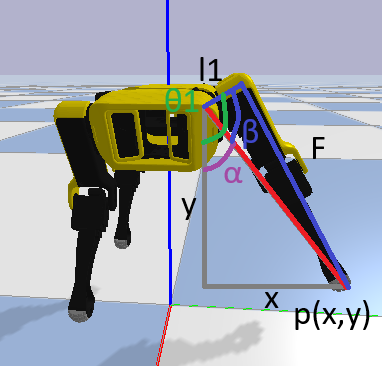
\includegraphics[width=0.85\textwidth]{images/y_z_view_ik.png}
    \caption{Όψη στο Y-Z επίπεδο}
    \label{fig:y_z_view_ik}
\end{figure}

\begin{figure}[htbp]
    \centering
    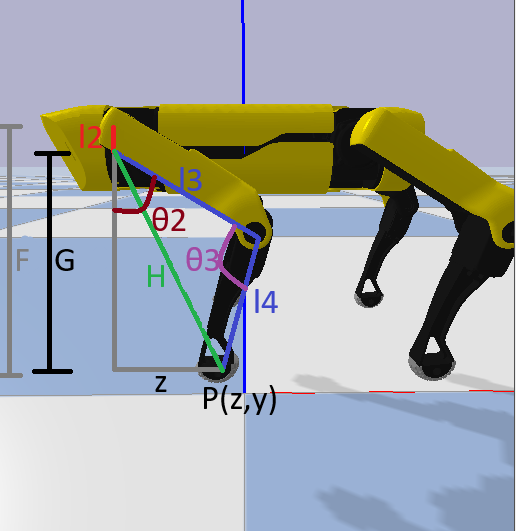
\includegraphics[width=0.85\textwidth]{images/x_y_view_ik.png}
    \caption{Όψη στο X-Y επίπεδο}
    \label{fig:x_y_view_ik}
\end{figure}

\subsection{Μετασχηματισμός Σώματος}
\label{subsec:body-transform}
Έχοντας τις εξισώσεις ευθείας και αντίστροφης κινηματικής για το κάθε πόδι
ξεχωριστά ως προς το πλαίσιο αναφοράς πάνω στον ώμο, για να ολοκληρώσουμε το
κινηματικό μοντέλο του ρομπότ χρειαζόμαστε έναν τελευταίο μετασχηματισμό, ώστε
οι προηγούμενες εξισώσεις να έχουν πλαίσιο αναφοράς το γεωμετρικό κέντρο του
σκελετού του ρομπότ. Ο μετασχηματισμός αυτός αποτελείται από μια μετατόπιση και
μια περιστροφή, και εκφράζεται συμπαγώς με έναν ομογενή πίνακα
\cite{siciliano_robotics_2009,sen_inverse_2017}.

Η στάση του σώματος περιγράφεται από τη θέση του κέντρου του
$\mathbf{p}_m = [x_m\ \ y_m\ \ z_m]^{T}$ και από τις τρεις γωνίες
προσανατολισμού: την $\omega$ (roll) περί τον άξονα $X$, την $\psi$ (pitch) περί
τον άξονα $Z$ και την $\phi$ (yaw) περί τον άξονα $Y$, σύμφωνα με το κινηματικό
πλαίσιο της ενότητας~\ref{sec:coord-frames}. Ο πίνακας στροφής προκύπτει από τη
σύνθεση των τριών επιμέρους στροφών,
\begin{equation}
R = R_x(\omega)\, R_y(\phi)\, R_z(\psi),
\label{eq:body-rot}
\end{equation}
και ο πλήρης μετασχηματισμός της στάσης του σώματος είναι
\begin{equation}
T_m =
\begin{bmatrix}
R & \mathbf{p}_m \\
\mathbf{0}^{T} & 1
\end{bmatrix}.
\label{eq:body-Tm}
\end{equation}

Κάθε ώμος βρίσκεται σε σταθερή θέση ως προς το κέντρο του σώματος, στις τέσσερις
γωνίες ενός ορθογωνίου με πλευρές $L$ και $W$. Ο μετασχηματισμός από το πλαίσιο
του σώματος στο πλαίσιο του $i$-οστού ώμου είναι επομένως
\begin{equation}
T^{(i)}_{\text{ώμου}} = T_m
\begin{bmatrix}
0 & 0 & 1 & \pm L/2 \\
0 & 1 & 0 & 0 \\
-1 & 0 & 0 & \pm W/2 \\
0 & 0 & 0 & 1
\end{bmatrix},
\label{eq:hip-transform}
\end{equation}
όπου τα πρόσημα $\pm L/2$ και $\pm W/2$ επιλέγονται ανάλογα με το σκέλος:
θετικό $L/2$ για τα εμπρός, αρνητικό για τα πίσω, θετικό $W/2$ για τα αριστερά
και αρνητικό για τα δεξιά. Το σταθερό τμήμα της \eqref{eq:hip-transform}
περιλαμβάνει, πέρα από τη μετατόπιση, και τη στροφή κατά $\pi/2$ περί τον άξονα
$Y$ που αναφέρθηκε στην \eqref{eq:shoulder-frame}: αυτή ακριβώς η στροφή παράγει
το τοπικό πλαίσιο του ώμου στο οποίο ισχύουν οι σχέσεις των δύο προηγούμενων
υποενοτήτων.

Ο μετασχηματισμός αυτός είναι που επιτρέπει τον ανεξάρτητο χειρισμό της στάσης
του σώματος: μεταβάλλοντας τα $\mathbf{p}_m$, $\omega$, $\psi$ και $\phi$ ενώ τα
πέλματα παραμένουν ακίνητα στο έδαφος, το σώμα μετατοπίζεται και περιστρέφεται
πάνω από σταθερά σημεία στήριξης, με τις γωνίες των αρθρώσεων να προκύπτουν
αυτόματα από την αντίστροφη κινηματική κάθε σκέλους. Στην υλοποίηση προβλέπεται
επιπλέον μια
σταθερή μετατόπιση του κέντρου αναφοράς ως προς το γεωμετρικό κέντρο, ώστε να
μπορεί να ληφθεί υπόψη η πραγματική θέση του κέντρου μάζας· στην παρούσα εργασία
η μετατόπιση αυτή είναι μηδενική. Για ομαλό χειρισμό της στάσης του σώματος ενώ
το ρομπότ βρίσκεται ακίνητο αναπτύχθηκαν ομαλές τροχιές στον χώρο των αρθρώσεων,
όπως θα δούμε στην ενότητα~\ref{sec:joint-space-traj}.

Το σύνολο των σχέσεων του κινηματικού μοντέλου που παρουσιάστηκαν στην ενότητα
αυτή υλοποιείται στον κώδικα της εργασίας, η δομή του οποίου αναλύεται στην
ενότητα~\ref{sec:software-architecture}.

\begin{figure}[htbp]
    \centering
    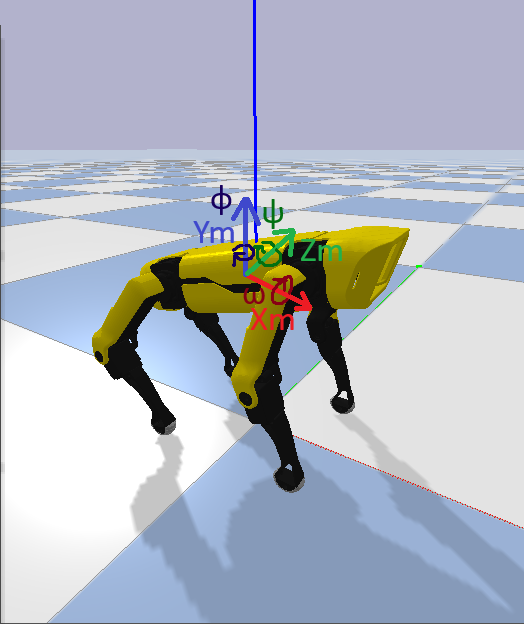
\includegraphics[width=0.85\textwidth]{images/bodyIK.png}
    \caption{Το τετράποδο με ελαφρά γωνία pitch και πλαίσιο αναφοράς στο
    γεωμετρικό κέντρο του σκελετού του ρομπότ}
    \label{fig:bodyIK}
\end{figure}

\section{Οπτικοποίηση και Επαλήθευση του Κινηματικού Μοντέλου}
\label{sec:matplotlib-vis}
Για την ταχεία επαλήθευση του κινηματικού μοντέλου, πριν από τη μετάβαση στη
δυναμική προσομοίωση και στο πραγματικό ρομπότ, αναπτύχθηκε ένα απλό εργαλείο
οπτικοποίησης σε Matplotlib. Το εργαλείο σχεδιάζει σε τρεις διαστάσεις το σώμα
του ρομπότ και τις τέσσερις κινηματικές αλυσίδες των σκελών, όπως προκύπτουν
από την ευθεία κινηματική για ένα δεδομένο σύνολο γωνιών άρθρωσης ή, αντίστροφα,
από την αντίστροφη κινηματική για δεδομένες θέσεις των άκρων. Με τον τρόπο αυτό,
σφάλματα στη γεωμετρία, στους μετασχηματισμούς ή στη στάση του σώματος
εντοπίζονται άμεσα οπτικά, χωρίς την υπολογιστική επιβάρυνση και τον χρόνο
προετοιμασίας μιας πλήρους δυναμικής προσομοίωσης.

\begin{figure}[htbp]
    \centering
    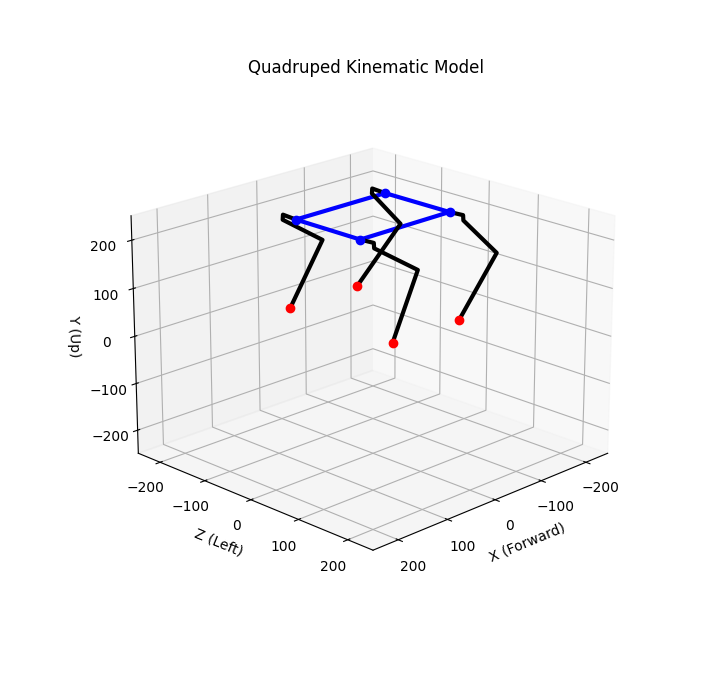
\includegraphics[width=0.85\textwidth]{images/matplotlib_sim.png}
    \caption{Οπτικοποίηση του κινηματικού μοντέλου σε Matplotlib: σώμα και
    κινηματικές αλυσίδες των τεσσάρων σκελών}
    \label{fig:matplotlib-kinematics-vis}
\end{figure}



% --- Gait Design ---
\chapter{Σχεδιασμός Τροχιών και Βάδισης}
Με το ολοκληρωμένο κινηματικό μοντέλο από το προηγούμενο κεφάλαιο, μπορούμε να προχωρήσουμε 
στον σχεδιασμό τροχιών με σκοπό την πραγματοποίηση κίνησης.
Σε αυτό το κεφάλαιο παρουσιάζονται τροχιές στον χώρο δράσης (operational space)
σχεδιασμένες για όλα τα είδη βάδισης, καθώς και τροχιές στον χώρο αρθρώσεων
(joint space) για ομαλό χειρισμό του σώματος, αξιοποιώντας τον μετασχηματισμό
σώματος που εισήχθη στην ενότητα~\ref{subsec:body-transform}.

\section{Σχεδιασμός Τροχιάς στον Χώρο Αρθρώσεων για Χειρισμό Σώματος}
\label{sec:joint-space-traj}
Το πρόβλημα ανήκει στην κατηγορία της κίνησης από σημείο σε σημείο
(point-to-point motion) στον χώρο των αρθρώσεων, όπου ζητείται η μετάβαση από
μια αρχική σε μια τελική διαμόρφωση εντός δεδομένου χρόνου, χωρίς να ενδιαφέρει
η ακριβής διαδρομή που διαγράφει το άκρο στον χώρο δράσης. Οι βασικές
απαιτήσεις μιας τέτοιας τροχιάς είναι να μην είναι υπολογιστικά απαιτητική και
οι θέσεις και οι ταχύτητες των αρθρώσεων να αποτελούν συνεχείς συναρτήσεις του
χρόνου \cite{siciliano_robotics_2009}.

Για ομαλές μεταβολές μεταξύ διαφορετικών διαμορφώσεων του σκελετού του ρομπότ,
π.χ. για μια μετάβαση από γωνίες $\text{RPY} = (0^\circ, 0^\circ, 0^\circ)$ σε
$\text{RPY} = (0^\circ, 20^\circ, 0^\circ)$, υπολογίζεται πρώτα η αρχική
κατάσταση του ρομπότ με βάση τις τρέχουσες γωνίες RPY του σκελετού.
Αξιοποιώντας το κινηματικό μοντέλο του προηγούμενου κεφαλαίου, προκύπτει η
αρχική διαμόρφωση $\mathbf{q}_0 \in \mathbb{R}^{12}$ στον χώρο των αρθρώσεων για
όλα τα πόδια του ρομπότ. Με παρόμοια διαδικασία προκύπτει και η επιθυμητή
διαμόρφωση $\mathbf{q}_f$. Η μετάβαση από τη μια κατάσταση στην άλλη γίνεται με
ημιτονοειδή παρεμβολή.

Συγκεκριμένα, για συνολική διάρκεια μετάβασης $T$ ορίζεται ο αδιάστατος
συντελεστής ράμπας
\begin{equation}
s(t) = \frac{1}{2}\left(1 - \cos\frac{\pi t}{T}\right), \qquad t \in [0,\,T],
\label{eq:cosine-ramp}
\end{equation}
και η διαμόρφωση των αρθρώσεων σε κάθε χρονική στιγμή δίνεται από τη γραμμική
παρεμβολή
\begin{equation}
\mathbf{q}(t) = \mathbf{q}_0 + s(t)\left(\mathbf{q}_f - \mathbf{q}_0\right).
\label{eq:joint-interp}
\end{equation}

Η επιλογή του συνημιτονοειδούς προφίλ της \eqref{eq:cosine-ramp} έναντι μιας
απλής γραμμικής ράμπας δικαιολογείται από τη γωνιακή ταχύτητα των αρθρώσεων,
η οποία προκύπτει με παραγώγιση της \eqref{eq:joint-interp}:
\begin{equation}
\dot{\mathbf{q}}(t) = \frac{\pi}{2T}\,\sin\!\left(\frac{\pi t}{T}\right)
\left(\mathbf{q}_f - \mathbf{q}_0\right).
\label{eq:joint-vel}
\end{equation}
Ισχύει $s(0) = 0$ και $s(T) = 1$, επομένως τα δύο άκρα της τροχιάς
επιτυγχάνονται ακριβώς, ενώ ταυτόχρονα $\dot{s}(0) = \dot{s}(T) = 0$, δηλαδή η
κίνηση ξεκινά και τερματίζει με μηδενική γωνιακή ταχύτητα. Έτσι αποφεύγονται οι
απότομες εντολές θέσης στους σερβοκινητήρες στην αρχή και στο τέλος της
μετάβασης. Η μέγιστη ταχύτητα εμφανίζεται στο μέσο της κίνησης, για $t = T/2$,
και ισούται με $\pi/2 \approx 1{,}57$ φορές τη μέση ταχύτητα
$(\mathbf{q}_f - \mathbf{q}_0)/T$.

Σημειώνεται ότι η γωνιακή επιτάχυνση, $\ddot{\mathbf{q}}(t) =
(\pi^2/2T^2)\cos(\pi t/T)(\mathbf{q}_f - \mathbf{q}_0)$, δεν μηδενίζεται στα
άκρα. Για τις ανάγκες της παρούσας εργασίας αυτό δεν αποτελεί περιορισμό, καθώς
οι μεταβάσεις εκτελούνται με το ρομπότ ακίνητο και με τυπική διάρκεια
$T = 0{,}5$~s. Η συνέχεια και της επιτάχυνσης αποτελεί πρόσθετη απαίτηση που
μπορεί να επιβληθεί \cite{siciliano_robotics_2009}, θα απαιτούσε όμως πολυώνυμο
ανώτερης τάξης.

Επειδή ο ίδιος συντελεστής $s(t)$ εφαρμόζεται και στις δώδεκα αρθρώσεις, όλες
ξεκινούν και τερματίζουν ταυτόχρονα, γεγονός που εξασφαλίζει συντονισμένη
κίνηση ολόκληρου του σώματος. Ως συνέπεια της παρεμβολής στον χώρο των
αρθρώσεων, η τροχιά που διαγράφει κάθε πέλμα στον καρτεσιανό χώρο δεν είναι
ευθύγραμμη· στη συγκεκριμένη εφαρμογή αυτό είναι αδιάφορο, αφού τα πέλματα
παραμένουν ακίνητα στο έδαφος και μεταβάλλεται μόνο η στάση του σώματος πάνω από
αυτά. Η διαδικασία υλοποιείται στον κώδικα της εργασίας
(ενότητα~\ref{sec:software-architecture}).

Στην πράξη, η τροχιά αυτή αποδείχθηκε απαραίτητη σε μία κυρίως περίπτωση, κατά
την εκκίνηση του ρομπότ. Πριν από την ενεργοποίηση των σερβοκινητήρων, το ρομπότ
τοποθετείται χειροκίνητα σε μια στάση κατά προσέγγιση γνωστών γωνιών, η οποία
όμως δεν ταυτίζεται με την αρχική διαμόρφωση του συστήματος ελέγχου. Χωρίς
ενδιάμεση παρεμβολή, η πρώτη κιόλας εντολή θέσης θα προκαλούσε απότομη μετάβαση
όλων των αρθρώσεων στην αρχική διαμόρφωση, με κίνδυνο μηχανικής καταπόνησης και
απώλειας ισορροπίας. Η ομαλή μετάβαση των σχέσεων
\eqref{eq:cosine-ramp} και \eqref{eq:joint-interp} καλύπτει ακριβώς αυτό το
κενό. Αυτούσιες μεταβολές της στάσης του σκελετού, όπως για παράδειγμα από
γωνία pitch $0^\circ$ σε $30^\circ$, δοκιμάστηκαν επιτυχώς για κάθε περίπτωση,
δεν αντιστοιχίστηκαν ωστόσο σε κάποιο πλήκτρο του χειριστηρίου και επομένως δεν
αξιοποιούνται κατά την κανονική λειτουργία.

\begin{figure}[htbp]
    \centering
    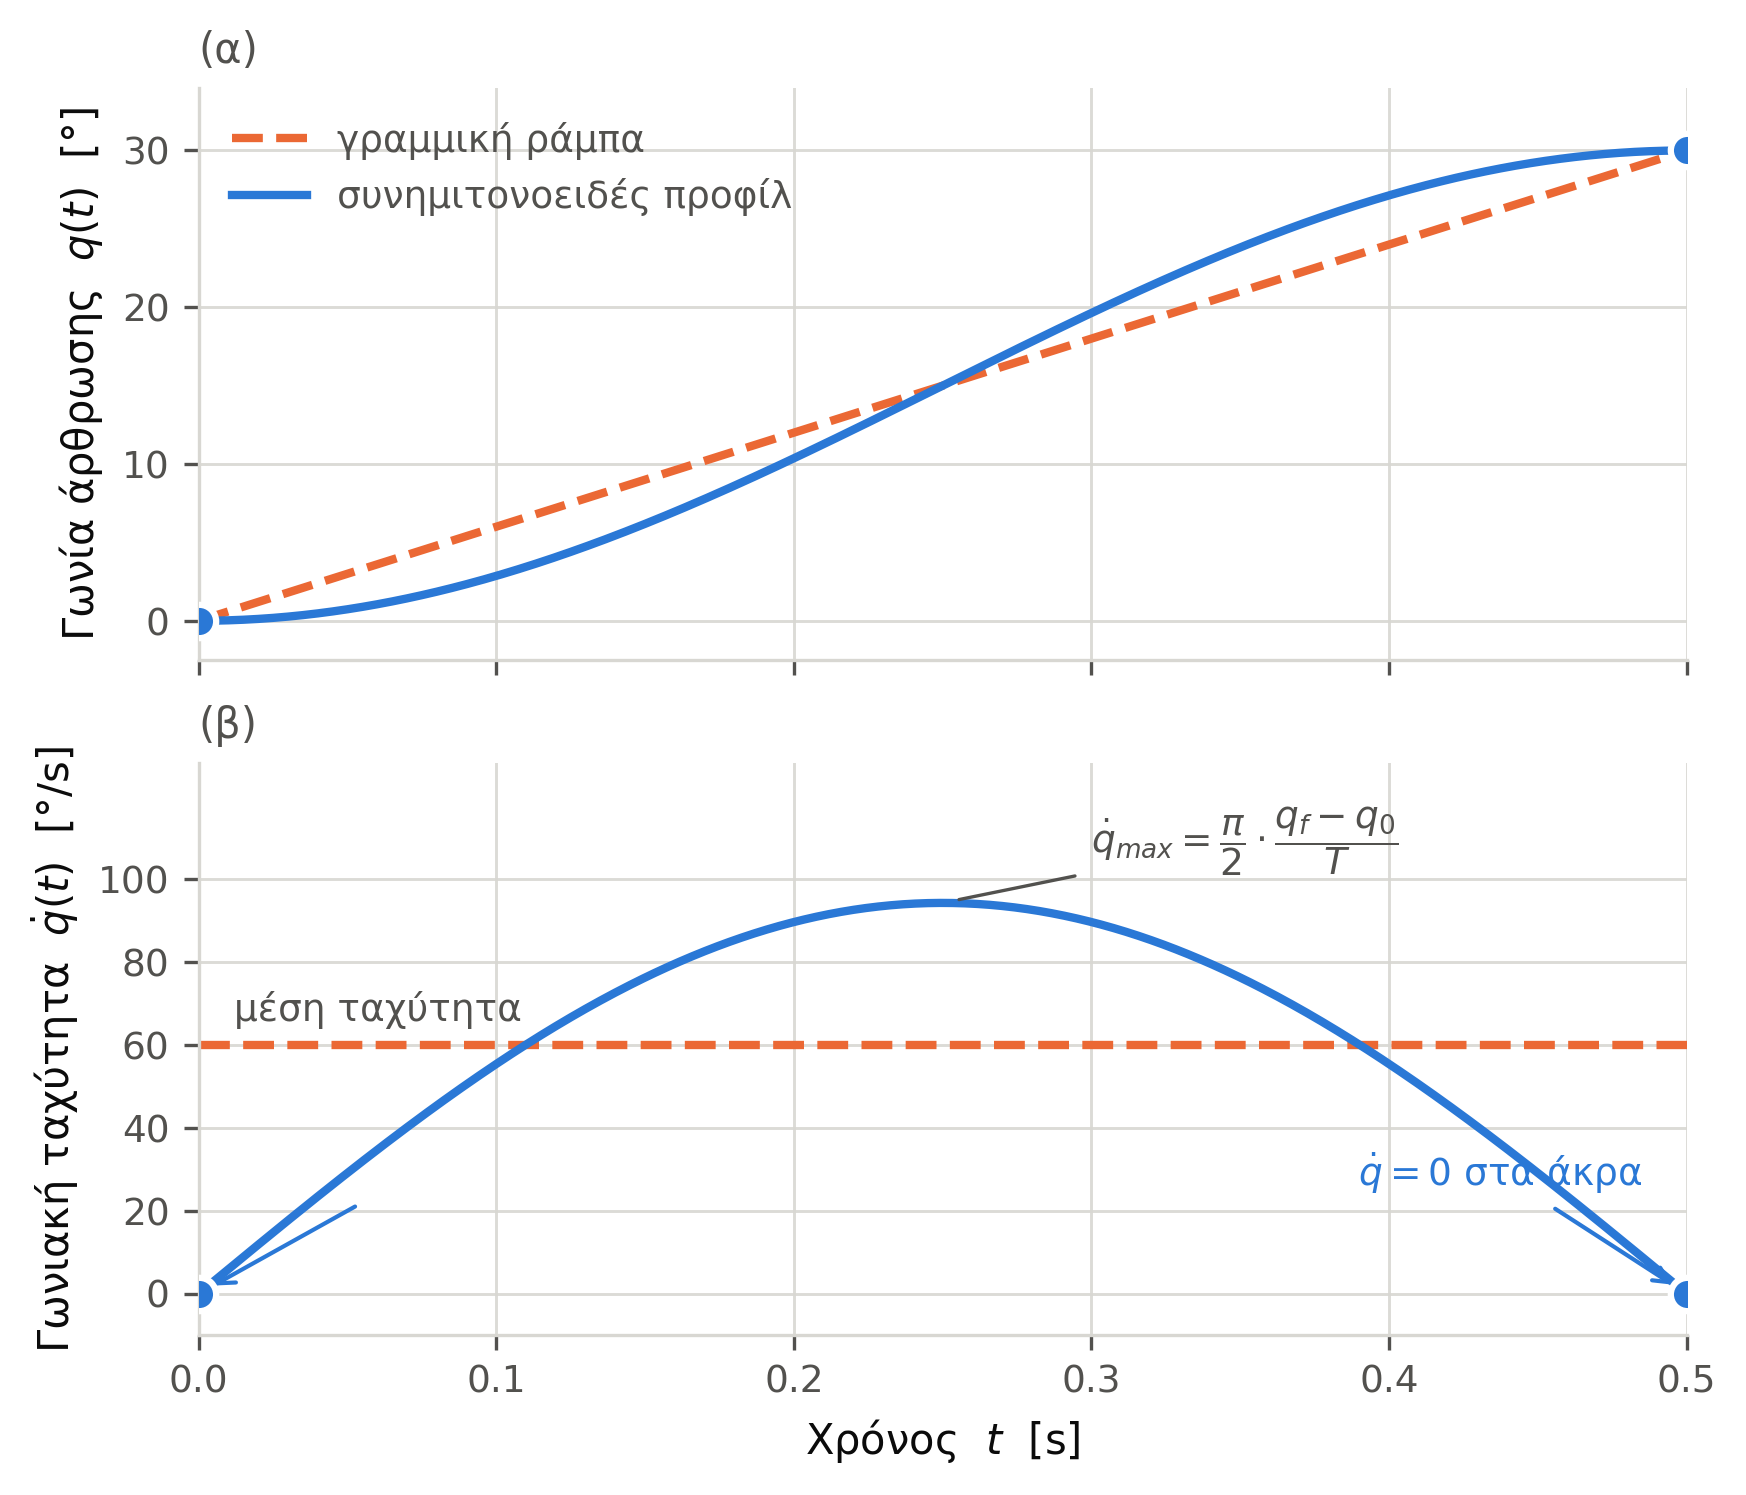
\includegraphics[width=0.8\textwidth]{images/joint_space_ramp.png}
    \caption[Συνημιτονοειδές προφίλ μετάβασης στον χώρο των αρθρώσεων]{Μετάβαση
    άρθρωσης κατά $30^\circ$ σε $T = 0{,}5$~s. (α) Γωνία $q(t)$ με το
    συνημιτονοειδές προφίλ της \eqref{eq:cosine-ramp} έναντι γραμμικής ράμπας.
    (β) Η αντίστοιχη γωνιακή ταχύτητα της \eqref{eq:joint-vel}: το
    συνημιτονοειδές προφίλ ξεκινά και τερματίζει με μηδενική ταχύτητα, με
    αντίτιμο μέγιστη ταχύτητα $\pi/2$ φορές τη μέση, ενώ η γραμμική ράμπα
    παρουσιάζει ασυνέχειες στα δύο άκρα}
    \label{fig:joint-trajectory-plot}
\end{figure}

\section{Σχεδιασμός Τροχιάς στον Καρτεσιανό Χώρο για Βάδιση}
Για την πραγματοποίηση οποιουδήποτε είδους βάδισης χρειάζεται επαρκής επίγνωση
της κίνησης του ποδιού στον καρτεσιανό χώρο, και για τον λόγο αυτό οι τροχιές
που ευθύνονται για τη βάδιση σχεδιάζονται στον καρτεσιανό χώρο (χώρος δράσης).
Η επιλογή είναι αντίθετη από εκείνη της ενότητας~\ref{sec:joint-space-traj} και
οφείλεται στη φύση των περιορισμών: ενώ στον χειρισμό της στάσης του σώματος η
διαδρομή του πέλματος είναι αδιάφορη, στη βάδιση η ίδια η γεωμετρία της
διαδρομής αποτελεί την προδιαγραφή. Το πόδι πρέπει να απομακρυνθεί επαρκώς από
το έδαφος ώστε να μην προσκρούσει σε αυτό κατά την αιώρηση, και να προσγειωθεί
σε συγκεκριμένο σημείο. Τέτοιοι περιορισμοί διαδρομής εκφράζονται φυσικά στον
χώρο δράσης, ενώ στον χώρο των αρθρώσεων τα αντίστοιχα σημεία είναι δύσκολο να
υπολογιστούν \cite{siciliano_robotics_2009}. Ο κύκλος βάδισης χωρίζεται στις δύο
φάσεις που ορίστηκαν στην ενότητα~\ref{subsec:gait-phases}, οι οποίες έχουν
διαφορετικές απαιτήσεις και επομένως σχεδιάζονται με διαφορετικές καμπύλες.

\subsection{Καμπύλες Bezier}
Οι καμπύλες Bezier είναι παραμετρικές καμπύλες που ορίζονται από ένα σύνολο
σημείων ελέγχου (control points). Στην παρούσα εργασία αξιοποιούνται για τον
σχεδιασμό της τροχιάς αιώρησης, για τους λόγους που αναπτύσσονται στην
ενότητα~\ref{subsec:swing-phase}. Στη συνέχεια παρουσιάζεται η μαθηματική τους
διατύπωση και οι ιδιότητες που καθιστούν δυνατό τον έλεγχο της τροχιάς.

Το πλεονέκτημα των καμπυλών αυτών είναι ότι το σχήμα τους καθορίζεται
αποκλειστικά από τη θέση των σημείων ελέγχου, χωρίς να απαιτείται επίλυση
κάποιου συστήματος εξισώσεων ή αριθμητική βελτιστοποίηση. Όπως θα φανεί
παρακάτω, οι ιδιότητες των πολυωνύμων Bernstein στα οποία στηρίζονται επιτρέπουν
τον έλεγχο όχι μόνο του σχήματος της καμπύλης, αλλά και της ταχύτητας και της
επιτάχυνσης στα άκρα της, μέσω της απλής επανάληψης σημείων ελέγχου.

Στην απλούστερη μορφή της, για δύο σημεία ελέγχου, η καμπύλη εκφυλίζεται σε
γραμμική παρεμβολή μεταξύ τους,
\begin{equation}
\mathbf{p}(t) = (1-t)\,\mathbf{p}_0 + t\,\mathbf{p}_1, \qquad t \in [0,1].
\label{eq:bezier-linear}
\end{equation}
Με τρία σημεία ελέγχου προκύπτει η τετραγωνική καμπύλη
\begin{equation}
\mathbf{p}(t) = (1-t)^{2}\,\mathbf{p}_0 + 2(1-t)t\,\mathbf{p}_1 + t^{2}\,\mathbf{p}_2,
\label{eq:bezier-quadratic}
\end{equation}
και με τέσσερα η κυβική
\begin{equation}
\mathbf{p}(t) = (1-t)^{3}\,\mathbf{p}_0 + 3(1-t)^{2}t\,\mathbf{p}_1
+ 3(1-t)t^{2}\,\mathbf{p}_2 + t^{3}\,\mathbf{p}_3.
\label{eq:bezier-cubic}
\end{equation}

Το μοτίβο των συντελεστών στις \eqref{eq:bezier-linear} έως
\eqref{eq:bezier-cubic} είναι το ανάπτυγμα του διωνύμου, γεγονός που οδηγεί
απευθείας στη γενική μορφή. Για $n+1$ σημεία ελέγχου
$\mathbf{p}_0, \dots, \mathbf{p}_n$, η καμπύλη Bezier $n$-οστού βαθμού είναι
\begin{equation}
\mathbf{p}(t) = \sum_{i=0}^{n} \binom{n}{i}(1-t)^{\,n-i}\,t^{\,i}\,\mathbf{p}_i,
\qquad t \in [0,1],
\label{eq:bezier-n}
\end{equation}
όπου ο συντελεστής κάθε σημείου ελέγχου
\begin{equation}
B_i^{n}(t) = \binom{n}{i}(1-t)^{\,n-i}\,t^{\,i}
\label{eq:bernstein}
\end{equation}
είναι το $i$-οστό πολυώνυμο Bernstein βαθμού $n$. Η
\eqref{eq:bezier-n} γράφεται επομένως συνοπτικά ως
$\mathbf{p}(t) = \sum_{i=0}^{n} B_i^{n}(t)\,\mathbf{p}_i$, δηλαδή ως
σταθμισμένος μέσος όρος των σημείων ελέγχου με βάρη τα πολυώνυμα Bernstein. Η
ίδια διατύπωση χρησιμοποιείται και στη γεννήτρια τροχιάς του MIT Cheetah
\cite{hyun_high_2014}.

Από τη μορφή αυτή προκύπτουν τρεις ιδιότητες που αξιοποιούνται άμεσα στον
σχεδιασμό της τροχιάς αιώρησης. Πρώτον, ισχύει
$\sum_{i=0}^{n} B_i^{n}(t) = 1$ με $B_i^{n}(t) \geq 0$, επομένως η καμπύλη
παραμένει πάντοτε εντός του κυρτού περιβλήματος (convex hull) των σημείων
ελέγχου· η τροχιά του πέλματος περιορίζεται έτσι σε γνωστή περιοχή του χώρου
εργασίας του σκέλους. Δεύτερον, $\mathbf{p}(0) = \mathbf{p}_0$ και
$\mathbf{p}(1) = \mathbf{p}_n$, δηλαδή τα σημεία απογείωσης και προσγείωσης
ορίζονται ακριβώς. Τρίτον, η παράγωγος της \eqref{eq:bezier-n} είναι και αυτή
καμπύλη Bezier, βαθμού $n-1$, με σημεία ελέγχου τις διαφορές των διαδοχικών
σημείων:
\begin{equation}
\dot{\mathbf{p}}(t) = n \sum_{i=0}^{n-1} B_i^{\,n-1}(t)
\left(\mathbf{p}_{i+1} - \mathbf{p}_i\right).
\label{eq:bezier-derivative}
\end{equation}

Η \eqref{eq:bezier-derivative} είναι το κλειδί για τον έλεγχο της ταχύτητας στα
άκρα. Στο $t = 0$ δίνει $\dot{\mathbf{p}}(0) = n(\mathbf{p}_1 - \mathbf{p}_0)$,
οπότε η επανάληψη του πρώτου σημείου ελέγχου, $\mathbf{p}_0 = \mathbf{p}_1$,
μηδενίζει την ταχύτητα κατά την απογείωση. Με αντίστοιχο συλλογισμό, η δεύτερη
παράγωγος στο $t = 0$ είναι ανάλογη της
$\mathbf{p}_2 - 2\mathbf{p}_1 + \mathbf{p}_0$, επομένως η τριπλή επανάληψη
$\mathbf{p}_0 = \mathbf{p}_1 = \mathbf{p}_2$ μηδενίζει και την επιτάχυνση. Το
ίδιο ισχύει συμμετρικά στο άλλο άκρο, για $t = 1$. Η τεχνική αυτή, η οποία
προαναφέρθηκε στην ενότητα~\ref{subsec:bezier-litreview}, επιτρέπει τη μηδενική
ταχύτητα και επιτάχυνση του πέλματος τη στιγμή της επαφής χωρίς καμία αλλαγή
στον αλγόριθμο, παρά μόνο με επανάληψη τιμών στη λίστα των σημείων ελέγχου.

\subsection{Φάση Swing}
\label{subsec:swing-phase}
Οι απαιτήσεις της φάσης αιώρησης είναι ταυτόχρονα γεωμετρικές και δυναμικές, και
αυτές ακριβώς οδήγησαν στην επιλογή καμπύλης Bezier. Γεωμετρικά, η τροχιά πρέπει
να εξασφαλίζει επαρκή απόσταση από το έδαφος, ώστε το πόδι να μην προσκρούσει σε
αυτό κατά την αιώρηση, και να καταλήγει στο επιθυμητό σημείο προσγείωσης.
Δυναμικά, πρέπει να είναι αρκετά ομαλή ώστε να μην προκαλεί απότομες μεταβολές
στη δυναμική του σκέλους, οι οποίες μπορούν να αποσταθεροποιήσουν ολόκληρο το
σώμα· η συνέχεια της θέσης, της ταχύτητας και της επιτάχυνσης, καθώς και η
ελαχιστοποίηση της μέγιστης επιτάχυνσης του σκέλους, αποτελούν καθιερωμένα
κριτήρια σχεδιασμού τροχιάς αιώρησης σε τετράποδα \cite{zeng_leg_2019}.
Ταυτόχρονα, ο ρυθμός με τον οποίο το πόδι κινείται προς τα πίσω λίγο πριν την
επαφή (swing leg retraction) επηρεάζει τις απώλειες ενέργειας κατά την
προσγείωση \cite{haberland}. Οι ίδιες ακριβώς απαιτήσεις οδήγησαν και τη
γεννήτρια τροχιάς του MIT Cheetah στην επιλογή καμπύλης Bezier
\cite{hyun_high_2014}.

Η τροχιά ορίζεται από δώδεκα σημεία ελέγχου, δηλαδή από καμπύλη ενδέκατου
βαθμού. Οι τιμές τους δίνονται κανονικοποιημένες στον
Πίνακα~\ref{tab:bezier-control-values} και αποτελούν παραλλαγή των τιμών της
πλατφόρμας SpotMiniMini \cite{spotminimini2020github}. Η κανονικοποιημένη
οριζόντια συντεταγμένη $x_n$ μετατρέπεται σε πραγματική μετατόπιση ως
\begin{equation}
d = \left(x_n - \tfrac{5}{6}\right) S,
\label{eq:swing-offset}
\end{equation}
όπου $S$ το μήκος βήματος, ενώ το ύψος προκύπτει ως $h = h_n H$ με $H$ το
ονομαστικό ύψος αιώρησης. Ο όρος $-5/6$ της \eqref{eq:swing-offset} τοποθετεί
την τροχιά ώστε η προσγείωση να συμβαίνει σε απόσταση $S/6$ μπροστά από την
ονομαστική θέση του πέλματος, σύμφωνα με τη μέθοδο βέλτιστης αρχικής θέσης
ποδιού για βάδισμα trot \cite{he_optimal_2020}.

Στα δύο άκρα, τόσο η οριζόντια όσο και η κατακόρυφη συντεταγμένη
επαναλαμβάνονται τρεις φορές. Σύμφωνα με την \eqref{eq:bezier-derivative}, η
επανάληψη αυτή μηδενίζει την ταχύτητα και την επιτάχυνση του πέλματος κατά την
απογείωση και κατά την προσγείωση, χωρίς καμία άλλη παρέμβαση στον αλγόριθμο.
Στο Σχήμα~\ref{fig:bezier-swing} οι τριπλές αυτές ομάδες εμφανίζονται ως ένα
σημείο η καθεμία, σημειωμένες με $\times 3$.

\begin{figure}[htbp]
    \centering
    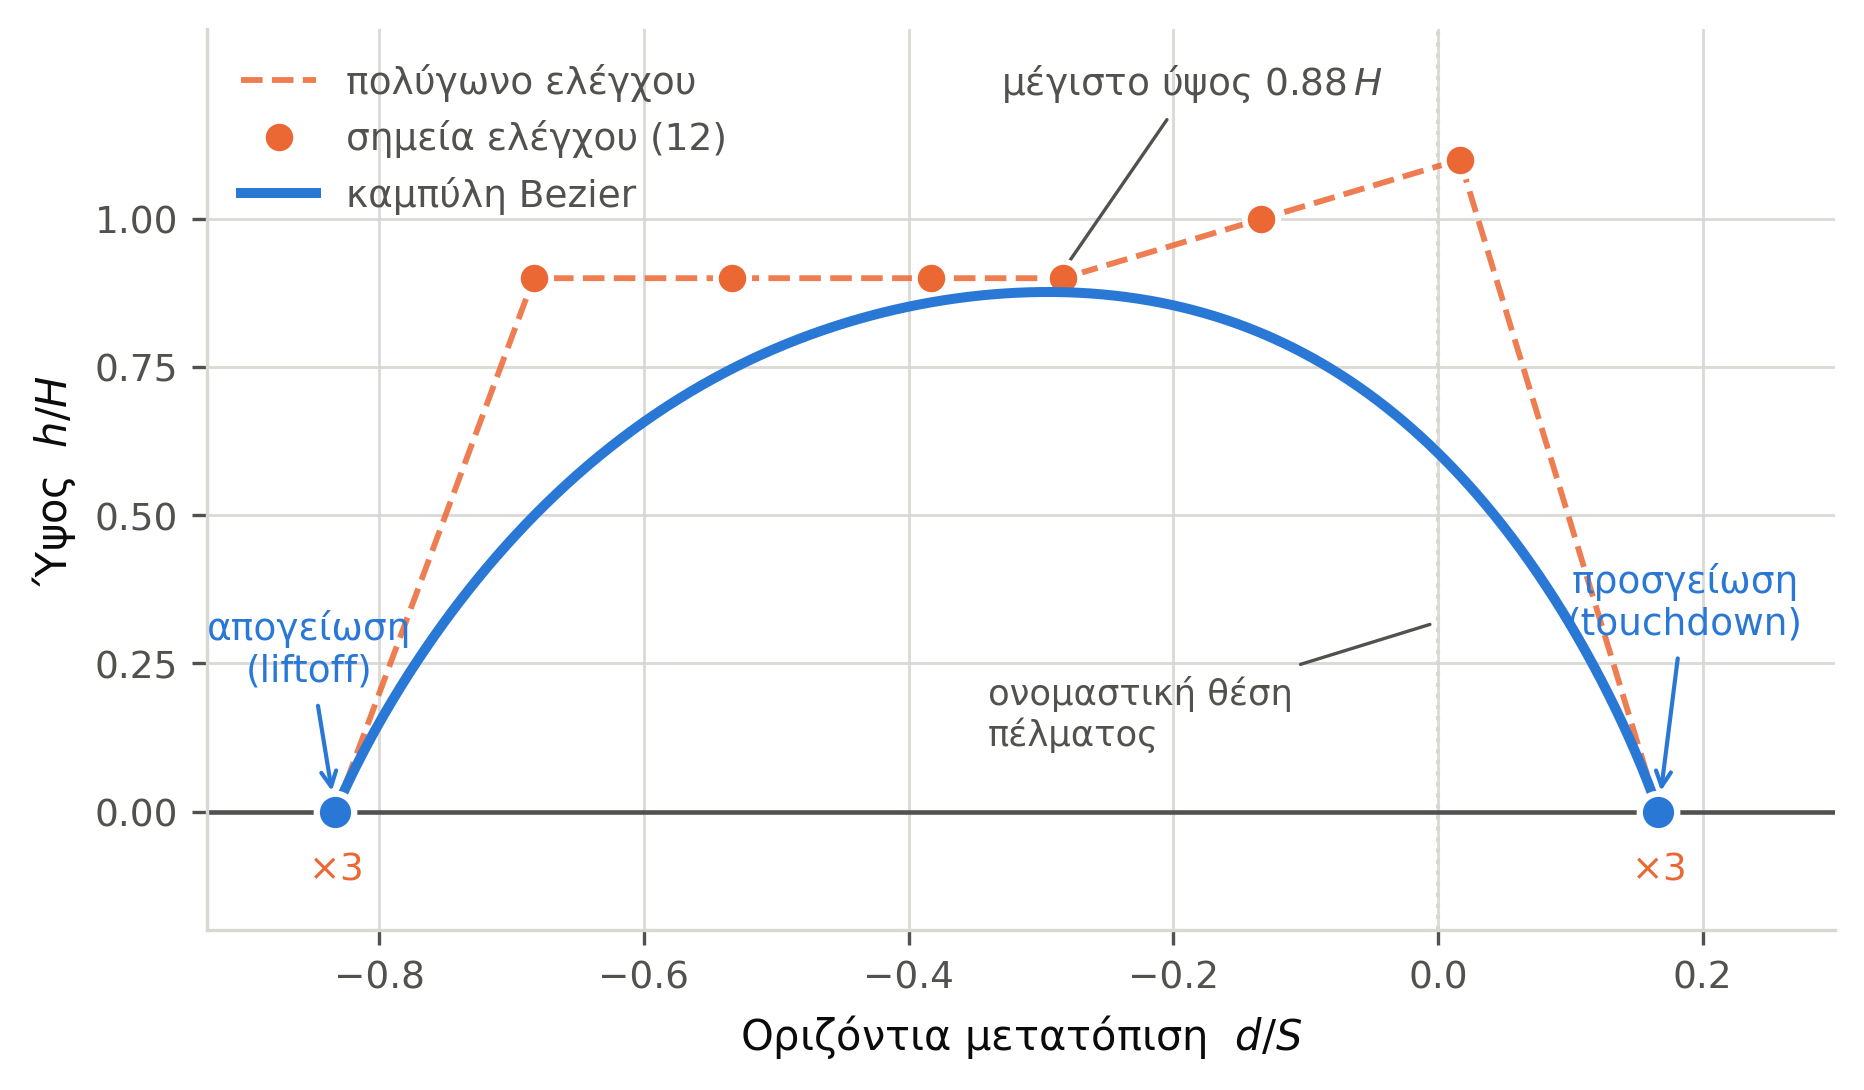
\includegraphics[width=0.92\textwidth]{images/bezier_swing.png}
    \caption[Τροχιά αιώρησης και σημεία ελέγχου Bezier]{Τροχιά του πέλματος
    κατά τη φάση αιώρησης, με τα δώδεκα σημεία ελέγχου και το πολύγωνο ελέγχου.
    Οι συντεταγμένες είναι κανονικοποιημένες ως προς το μήκος βήματος $S$ και το
    ύψος αιώρησης $H$. Οι τριπλά επαναλαμβανόμενες ομάδες στα άκρα σημειώνονται
    με $\times 3$}
    \label{fig:bezier-swing}
\end{figure}

\begin{table}[htbp]
    \centering
    \small
    \begin{tabular}{@{}l *{12}{c}@{}}
        \toprule
        $i$ & 0 & 1 & 2 & 3 & 4 & 5 & 6 & 7 & 8 & 9 & 10 & 11 \\
        \midrule
        $x_n$ & 0,00 & 0,00 & 0,00 & 0,15 & 0,30 & 0,45 & 0,55 & 0,70 & 0,85 & 1,00 & 1,00 & 1,00 \\
        $h_n$ & 0,00 & 0,00 & 0,00 & 0,90 & 0,90 & 0,90 & 0,90 & 1,00 & 1,10 & 0,00 & 0,00 & 0,00 \\
        \bottomrule
    \end{tabular}
    \caption[Κανονικοποιημένα σημεία ελέγχου Bezier της τροχιάς αιώρησης]{Οι
    κανονικοποιημένες τιμές των δώδεκα σημείων ελέγχου Bezier της τροχιάς
    αιώρησης, παραλλαγή των τιμών του SpotMiniMini
    \cite{spotminimini2020github}}
    \label{tab:bezier-control-values}
\end{table}

Αξίζει να σημειωθεί ότι το πολύγωνο ελέγχου που προκύπτει από τις τιμές αυτές
δεν είναι συμμετρικό και, σε πρώτη ανάγνωση, δεν φαίνεται διαισθητικό: η
κατακόρυφη συνιστώσα παρουσιάζει ένα οριζόντιο τμήμα στο $0{,}9H$, ανεβαίνει
έως το $1{,}1H$ και κατόπιν πέφτει απότομα στο μηδέν. Επειδή όμως η καμπύλη
Bezier δεν διέρχεται από τα ενδιάμεσα σημεία ελέγχου παρά μόνο έλκεται προς
αυτά, η τελική τροχιά είναι ομαλή και ικανοποιεί τις απαιτήσεις που τέθηκαν
παραπάνω. Χαρακτηριστικά, το πραγματικό μέγιστο ύψος της είναι $0{,}88H$ και όχι
$1{,}1H$, δηλαδή η παράμετρος $H$ λειτουργεί ως συντελεστής κλίμακας και όχι ως
απόλυτο ύψος. Οι τιμές διατηρήθηκαν ως έχουν, καθώς επαληθεύτηκαν πειραματικά
τόσο στην προσομοίωση όσο και στο πραγματικό ρομπότ.

\subsection{Φάση Stance}
\label{subsec:stance-phase}
Οι απαιτήσεις της φάσης στήριξης είναι εντελώς διαφορετικές από εκείνες της
αιώρησης και δεν δικαιολογούν την πολυπλοκότητα μιας καμπύλης Bezier. Το πέλμα
βρίσκεται σε επαφή με το έδαφος και οφείλει να παραμείνει ακίνητο ως προς αυτό,
κάτι που, εκφρασμένο στο πλαίσιο του σώματος, σημαίνει ότι πρέπει να κινείται
προς τα πίσω με σταθερή ταχύτητα ίση κατά μέτρο με την ταχύτητα προώθησης του
ρομπότ. Για τον λόγο αυτό υιοθετείται απλή παραμετρική τροχιά.

Για κανονικοποιημένη πρόοδο της φάσης $t \in [0,1]$, η οριζόντια μετατόπιση
είναι γραμμική,
\begin{equation}
d = \frac{S}{6} - t\,S,
\label{eq:stance-x}
\end{equation}
ενώ η κατακόρυφη ακολουθεί ημιτονοειδές προφίλ με πλάτος το βάθος διείσδυσης
$\delta$,
\begin{equation}
h = -\,\delta \sin(\pi t).
\label{eq:stance-y}
\end{equation}
Η \eqref{eq:stance-x} εξασφαλίζει τη συνέχεια του κύκλου βάδισης: για $t = 0$
δίνει $d = +S/6$, δηλαδή ακριβώς το σημείο προσγείωσης στο οποίο καταλήγει η
τροχιά αιώρησης της \eqref{eq:swing-offset}, και για $t = 1$ δίνει $d = -5S/6$,
δηλαδή το σημείο απογείωσης από το οποίο αυτή ξεκινά. Οι δύο φάσεις κλείνουν
έτσι έναν συνεχή κύκλο, όπως φαίνεται στο
Σχήμα~\ref{fig:stance-sine}α.

Παραγωγίζοντας, η ταχύτητα του πέλματος κατά τη στήριξη είναι
\begin{equation}
\dot{d} = -\frac{S}{T_{st}}, \qquad
\dot{h} = -\,\frac{\delta \pi}{T_{st}} \cos(\pi t),
\label{eq:stance-vel}
\end{equation}
όπου $T_{st}$ η διάρκεια της φάσης στήριξης. Η οριζόντια συνιστώσα είναι
σταθερή, όπως απαιτείται ώστε το σώμα να μετατοπίζεται ομοιόμορφα πάνω από το
ακίνητο πέλμα.

Η επιλογή ημιτονοειδούς προφίλ με δύο μόνο παραμέτρους, το μήκος βήματος και το
πλάτος $\delta$, ακολουθεί τη γεννήτρια τροχιάς του MIT Cheetah
\cite{hyun_high_2014} και υιοθετείται και από την πλατφόρμα SpotMiniMini
\cite{spotminimini2020github}. Ο ρόλος του $\delta$ όμως διαφέρει. Στο MIT
Cheetah, όπου το σκέλος διαθέτει ελεγχόμενη ενδοτικότητα, το βάθος διείσδυσης
της τροχιάς αναφοράς κάτω από το επίπεδο του εδάφους χρησιμοποιείται για τη
ρύθμιση της δύναμης αντίδρασης που ασκεί το πόδι \cite{hyun_high_2014}. Στην
παρούσα εργασία, με σερβοκινητήρες θέσης χωρίς ανάδραση δύναμης, κάτι τέτοιο
δεν είναι εφικτό· εδώ το $\delta$ εξασφαλίζει απλώς ότι το πέλμα διατηρεί
συνεχή επαφή με το έδαφος καθ' όλη τη διάρκεια της στήριξης, απορροφώντας
μικρές ανωμαλίες του δαπέδου και σφάλματα θέσης των σερβοκινητήρων. Στην
υλοποίηση το $\delta$ δεν είναι σταθερό, αλλά αυξάνεται ανάλογα με τη διόρθωση
ύψους που επιβάλλει ο ελεγκτής σταθεροποίησης ανά πόδι
(ενότητα~\ref{sec:stabilization}), ώστε η επαφή να διατηρείται και σε κεκλιμένο
έδαφος.

\begin{figure}[htbp]
    \centering
    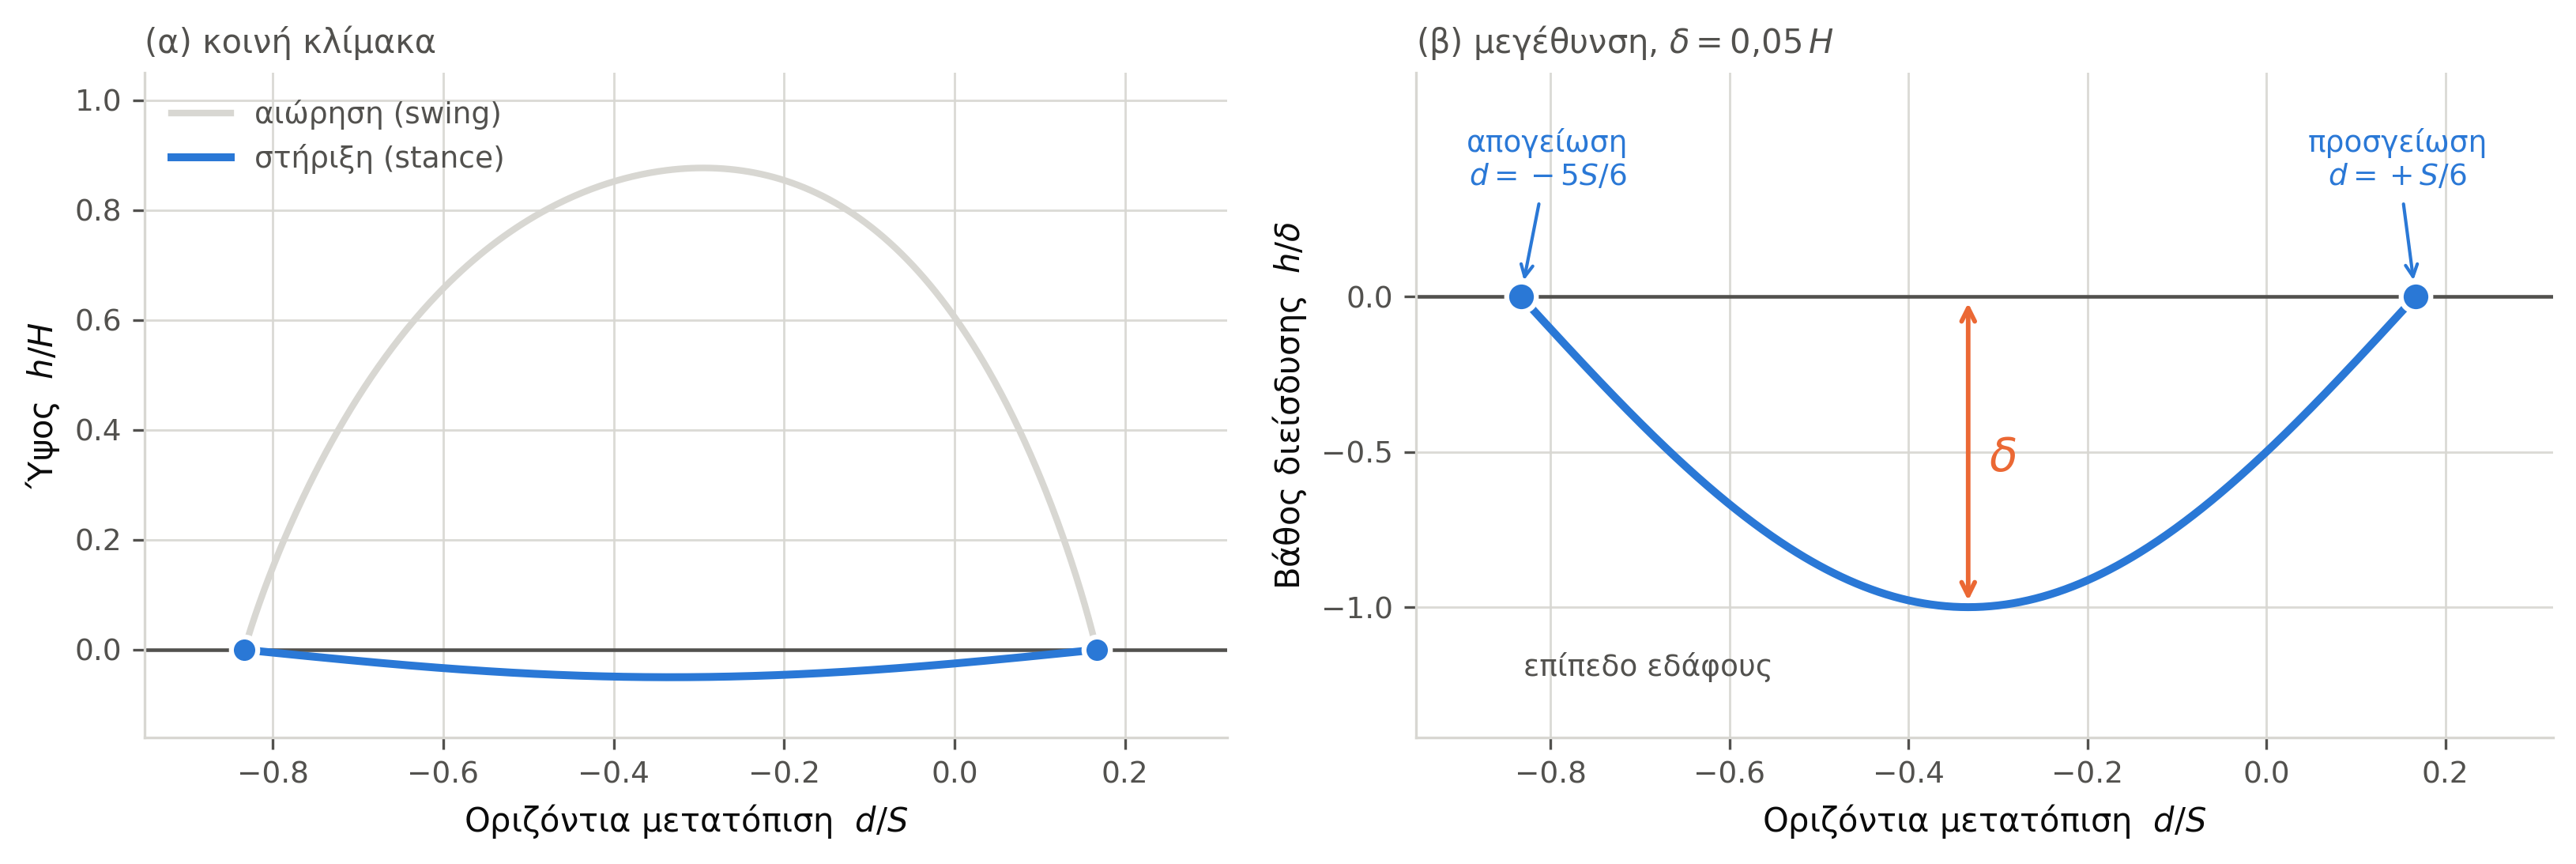
\includegraphics[width=\textwidth]{images/stance_sine.png}
    \caption[Ημιτονοειδής τροχιά στήριξης με βάθος διείσδυσης]{Τροχιά του
    πέλματος κατά τη φάση στήριξης. (α) Οι δύο φάσεις σε κοινή κλίμακα: η
    στήριξη είναι σχεδόν επίπεδη σε σύγκριση με την αιώρηση και κλείνει τον
    κύκλο στα ίδια ακριβώς άκρα. (β) Μεγέθυνση της στήριξης, όπου φαίνεται το
    ημιτονοειδές προφίλ και το βάθος διείσδυσης $\delta$}
    \label{fig:stance-sine}
\end{figure}

Σημειώνεται τέλος ότι η μετάβαση μεταξύ των δύο φάσεων είναι συνεχής ως προς τη
θέση, όχι όμως και ως προς την ταχύτητα. Η τροχιά αιώρησης φτάνει στο σημείο
προσγείωσης με μηδενική ταχύτητα, ενώ η \eqref{eq:stance-vel} επιβάλλει από την
πρώτη κιόλας στιγμή της στήριξης οριζόντια ταχύτητα $-S/T_{st}$. Η μηδενική
κατακόρυφη ταχύτητα κατά την επαφή περιορίζει την κρουστική φόρτιση, ωστόσο η
πλήρης αντιστοίχιση της ταχύτητας του πέλματος με εκείνη του εδάφους θα
απαιτούσε μη μηδενική ταχύτητα προσγείωσης, δηλαδή υλοποίηση swing leg
retraction \cite{haberland}, η οποία καταγράφεται ως μελλοντική επέκταση
(ενότητα~\ref{sec:future-work}).

\section{Βάδισμα Trot}
Το κύριο είδος βάδισης που αναπτύχθηκε σε βάθος και του οποίου δοκιμάστηκε η
πλήρης πανκατευθυντική λειτουργία είναι το trot. Όπως αναφέρθηκε στη
βιβλιογραφική ανασκόπηση (ενότητα~\ref{subsec:gait-phases}), η επιλογή του
οφείλεται στην ενεργειακή του αποδοτικότητα σε ευρύ φάσμα ταχυτήτων, στην ευρεία
χρήση του στη φύση και στη συμμετρία του, η οποία εξασφαλίζει ότι το διαγώνιο
ζεύγος που βρίσκεται σε επαφή στηρίζει το σώμα καθ' όλη τη διάρκεια του κύκλου
\cite{hu_trotting_2011,mori_study_2022}.

\subsection{Κατανομή Φάσεων Διαγώνιων Ζευγών}
Έχοντας σχεδιάσει τις δύο επιμέρους φάσεις που θα απαρτίσουν το βάδισμα, πρέπει
στη συνέχεια να αναπτυχθεί ένας τρόπος συγχρονισμού τους, ώστε να
πραγματοποιείται ομαλή κίνηση χωρίς απότομες διακοπές. Η κύρια πληροφορία που
απαιτείται είναι πότε τελειώνει η μία φάση και πότε πρέπει να αρχίσει η επόμενη,
καθώς και σε ποια χρονική στιγμή της φάσης βρισκόμαστε.

Και τα δύο ερωτήματα απαντώνται με την εισαγωγή μιας αδιάστατης μεταβλητής
φάσης. Αν $T_{sw}$ και $T_{st}$ είναι οι διάρκειες της αιώρησης και της
στήριξης αντίστοιχα, η περίοδος ενός πλήρους κύκλου βάδισης είναι
$T_{cyc} = T_{sw} + T_{st}$, και η καθολική φάση ορίζεται ως
\begin{equation}
\phi = \frac{t \bmod T_{cyc}}{T_{cyc}} \in [0,1).
\label{eq:global-phase}
\end{equation}
Η \eqref{eq:global-phase} είναι ουσιαστικά ένα πριονωτό σήμα που προωθείται από
ρολόι, αντίστοιχο με τα σήματα φάσης που παράγει ο διαμορφωτής προτύπου
βάδισης του MIT Cheetah \cite{hyun_high_2014}.

Κάθε πόδι δεν βρίσκεται στο ίδιο σημείο του κύκλου, αλλά μετατοπισμένο κατά μια
σταθερή διαφορά φάσης $\Delta S_i$ που καθορίζει το είδος του βαδίσματος:
\begin{equation}
\phi_i = \left(\phi + \Delta S_i\right) \bmod 1.
\label{eq:leg-phase}
\end{equation}
Ο διαχωρισμός ανάμεσα στις δύο φάσεις γίνεται με τον συντελεστή πλήρωσης (duty
factor)
\begin{equation}
\beta = \frac{T_{st}}{T_{cyc}},
\label{eq:duty-factor}
\end{equation}
ο οποίος εκφράζει το ποσοστό του κύκλου κατά το οποίο το πόδι βρίσκεται σε
επαφή με το έδαφος. Το πόδι $i$ βρίσκεται σε στήριξη όσο $\phi_i < \beta$ και σε
αιώρηση διαφορετικά, ενώ η πρόοδος εντός της εκάστοτε φάσης κανονικοποιείται
στο $[0,1]$ ως
\begin{equation}
t =
\begin{cases}
\dfrac{\phi_i}{\beta}, & \phi_i < \beta \quad \text{(στήριξη)} \\[10pt]
\dfrac{\phi_i - \beta}{1 - \beta}, & \phi_i \geq \beta \quad \text{(αιώρηση)}.
\end{cases}
\label{eq:phase-progress}
\end{equation}
Η μεταβλητή $t$ της \eqref{eq:phase-progress} είναι ακριβώς αυτή που
τροφοδοτείται στις \eqref{eq:stance-x} και \eqref{eq:swing-offset}, οπότε ο
χρονισμός συνδέεται άμεσα με τις τροχιές που σχεδιάστηκαν στην προηγούμενη
ενότητα.

Για το βάδισμα trot οι διαφορές φάσης είναι
$\Delta S = [0{,}0,\ 0{,}5,\ 0{,}5,\ 0{,}0]$ για τα πόδια FL, FR, RL και RR
αντίστοιχα. Τα διαγώνια ζεύγη FL+RR και FR+RL κινούνται επομένως σε αντίθεση
φάσης, με το ένα σε στήριξη όσο το άλλο αιωρείται, όπως φαίνεται στο
Σχήμα~\ref{fig:trot-phase}. Ως προς το πόδι αναφοράς FL, οι τιμές αυτές
ταυτίζονται με τη διάταξη $\Delta \vec{S}_{trot} = [0{,}5,\ 0{,}5,\ 0]$ του MIT
Cheetah \cite{hyun_high_2014}, ενώ την ίδια λογική χρονοπρογραμματισμού φάσεων
ακολουθεί και η υλοποίηση του SpotMiniMini \cite{spotminimini2020github}.

\begin{figure}[htbp]
    \centering
    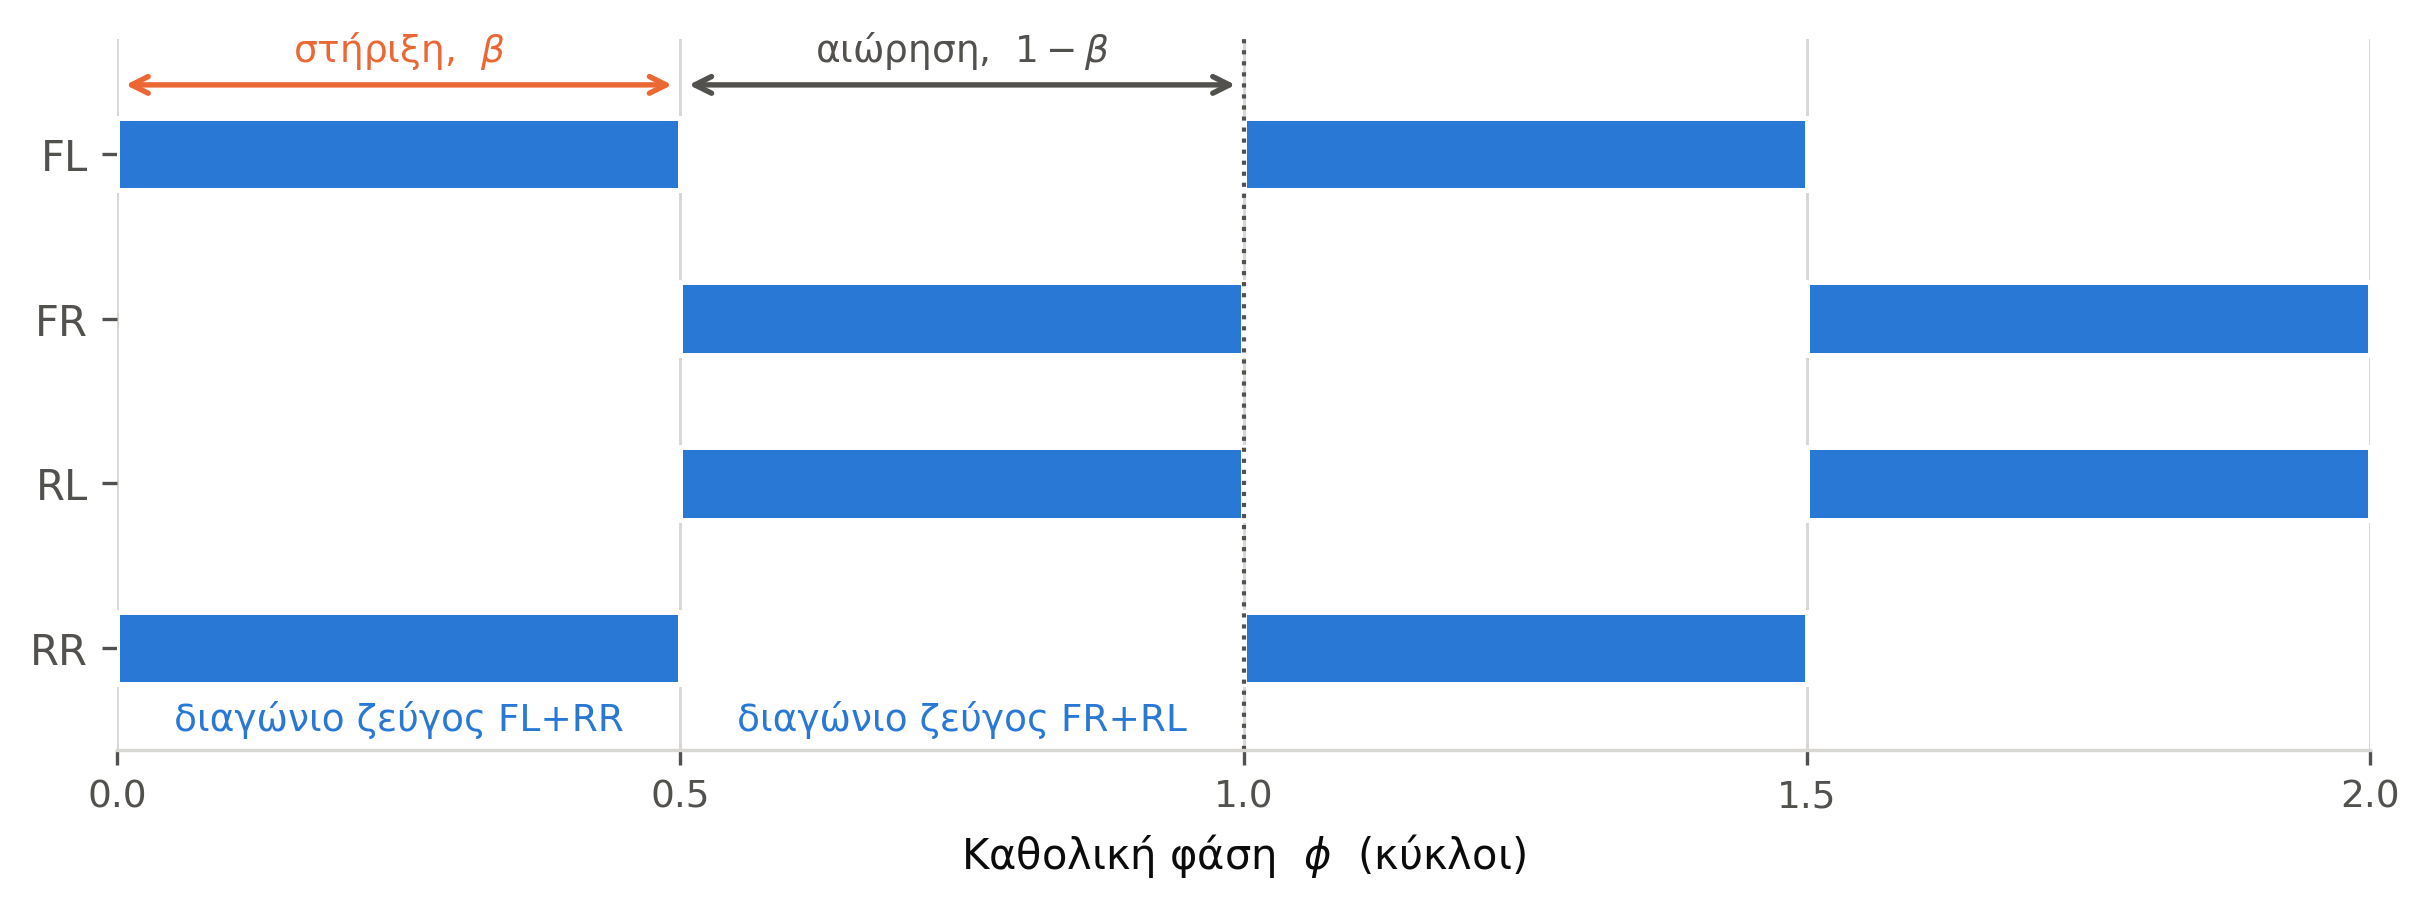
\includegraphics[width=0.95\textwidth]{images/trot_phase.png}
    \caption[Διάγραμμα φάσεων βαδίσματος trot]{Διάγραμμα φάσεων του βαδίσματος
    trot για δύο διαδοχικούς κύκλους. Οι γεμάτες περιοχές αντιστοιχούν σε φάση
    στήριξης. Τα διαγώνια ζεύγη FL+RR και FR+RL βρίσκονται σε αντίθεση φάσης,
    ενώ ο συντελεστής πλήρωσης $\beta$ καθορίζει το ποσοστό του κύκλου που κάθε
    πόδι βρίσκεται σε επαφή με το έδαφος}
    \label{fig:trot-phase}
\end{figure}

Ως προς τις διάρκειες, η υλοποίηση δεν κρατά και τις δύο σταθερές. Η διάρκεια
αιώρησης $T_{sw}$ ορίζεται σταθερή, καθώς περιορίζεται από την ταχύτητα
απόκρισης των σερβοκινητήρων, ενώ η διάρκεια στήριξης προκύπτει από την
επιθυμητή ταχύτητα $v$ και το μήκος διαδρομής στήριξης $S_{st}$ ως
\begin{equation}
T_{st} = \min\!\left(\frac{S_{st}}{|v|},\ 1{,}3\,T_{sw}\right).
\label{eq:tstance}
\end{equation}
Ο συντελεστής πλήρωσης της \eqref{eq:duty-factor} δεν είναι επομένως σταθερός,
αλλά μεταβάλλεται με την ταχύτητα: σε υψηλές ταχύτητες η στήριξη συντομεύει και
το $\beta$ μειώνεται, συμπεριφορά που παρατηρείται και στα ζώα. Το άνω όριο
$1{,}3\,T_{sw}$ αποτρέπει υπερβολικά αργούς κύκλους σε πολύ χαμηλές ταχύτητες.

Το βάδισμα καθορίζεται συνολικά από ένα μικρό σύνολο ρυθμιζόμενων παραμέτρων,
οι οποίες δίνονται ως είσοδος σε κάθε κλήση του βρόχου βάδισης. Από αυτές
προκύπτουν στη συνέχεια όλα τα υπόλοιπα μεγέθη του χρονισμού. Οι τιμές τους,
μαζί με τα παράγωγα μεγέθη και τις διαφορές φάσης, συνοψίζονται στον
Πίνακα~\ref{tab:trot-timing-params}. Αξίζει να σημειωθεί ότι το ονομαστικό ύψος
αιώρησης $H = 35$~mm δεν είναι το πραγματικό μέγιστο ύψος του πέλματος: όπως
προέκυψε στην ενότητα~\ref{subsec:swing-phase}, η καμπύλη Bezier φτάνει στο
$0{,}88H$, δηλαδή περίπου $31$~mm, ενώ το βάθος διείσδυσης της φάσης στήριξης
είναι $\delta = 0{,}05H \approx 1{,}8$~mm.

\begin{table}[htbp]
    \centering
    \small
    \begin{tabular}{@{}l l l@{}}
        \toprule
        Παράμετρος & Σύμβολο & Τιμή \\
        \midrule
        \multicolumn{3}{@{}l}{\textit{Ρυθμιζόμενες}} \\
        Επιθυμητή γραμμική ταχύτητα & $v$ & $0{,}30$ m/s$^{*}$ \\
        Επιθυμητή γωνιακή ταχύτητα & $\omega$ & $0{,}00$ rad/s$^{*}$ \\
        Ονομαστικό ύψος αιώρησης & $H$ & $35$ mm \\
        Μήκος διαδρομής στήριξης & $S_{st}$ & $60$ mm \\
        Διάρκεια αιώρησης & $T_{sw}$ & $0{,}25$ s \\
        Κατεύθυνση κίνησης & --- & $+x^{*}$ \\
        Είδος βαδίσματος & --- & trot \\
        \midrule
        \multicolumn{3}{@{}l}{\textit{Παράγωγες}} \\
        Διάρκεια στήριξης & $T_{st}$ & $\min\!\left(S_{st}/|v|,\ 1{,}3\,T_{sw}\right)$ \\
        Περίοδος κύκλου & $T_{cyc}$ & $T_{sw} + T_{st}$ \\
        Συντελεστής πλήρωσης & $\beta$ & $T_{st}/T_{cyc}$ \\
        Βάθος διείσδυσης & $\delta$ & $0{,}05\,H$ \\
        \midrule
        \multicolumn{3}{@{}l}{\textit{Διαφορές φάσης (trot)}} \\
        Εμπρός αριστερό & $\Delta S_{FL}$ & $0{,}0$ \\
        Εμπρός δεξί & $\Delta S_{FR}$ & $0{,}5$ \\
        Πίσω αριστερό & $\Delta S_{RL}$ & $0{,}5$ \\
        Πίσω δεξί & $\Delta S_{RR}$ & $0{,}0$ \\
        \bottomrule
    \end{tabular}
    \caption[Ρυθμιζόμενες και παράγωγες παράμετροι του βαδίσματος trot]{
    Ρυθμιζόμενες και παράγωγες παράμετροι του βαδίσματος trot. Οι τιμές που
    σημειώνονται με $^{*}$ είναι ενδεικτικές: η γραμμική και η γωνιακή ταχύτητα,
    καθώς και η κατεύθυνση, αποτελούν την εντολή κίνησης και μεταβάλλονται
    συνεχώς κατά τη λειτουργία ανάλογα με την επιθυμητή κίνηση}
    \label{tab:trot-timing-params}
\end{table}

Κατά την ανάπτυξη υλοποιήθηκαν τέσσερις παραλλαγές του σχήματος χρονισμού, οι
οποίες μοιράζονται τον ίδιο πυρήνα και διαφέρουν αποκλειστικά στον τρόπο με τον
οποίο προκύπτουν οι διάρκειες και το ρολόι της φάσης. Οι παραλλαγές αυτές
προέκυψαν από τη μελέτη των αντίστοιχων υλοποιήσεων του SpotMiniMini
\cite{spotminimini2020github} και του MIT Cheetah \cite{hyun_high_2014}:

\begin{itemize}
  \item \textbf{Σταθερή στήριξη.} Η περίοδος $T_{cyc}$ και ο συντελεστής
  πλήρωσης $\beta$ υπολογίζονται μία φορά από την ονομαστική ταχύτητα και
  παραμένουν σταθεροί, ενώ με την ταχύτητα μεταβάλλεται μόνο το μήκος βήματος.
  Επειδή ο χρονισμός δεν αλλάζει ποτέ, τα διαγώνια ζεύγη παραμένουν ακριβώς σε
  αντίθεση φάσης ανεξάρτητα από επιταχύνσεις ή στροφές.
  \item \textbf{Σταθερή αιώρηση με ελεύθερο ρολόι.} Η διάρκεια στήριξης
  προκύπτει από την τρέχουσα ταχύτητα κατά την \eqref{eq:tstance} και η φάση
  από την \eqref{eq:global-phase}. Η επιλογή αυτή ακολουθεί τη λογική του MIT
  Cheetah, όπου η περίοδος στήριξης καθορίζεται από την επιθυμητή ταχύτητα
  \cite{hyun_high_2014}, έχει όμως ως συνέπεια η περίοδος του κύκλου να
  μεταβάλλεται συνεχώς κατά τη διάρκεια της ράμπας ταχύτητας.
  \item \textbf{Σταθερή αιώρηση με επαναφορά στην επαφή.} Παραλλαγή της
  προηγούμενης, στην οποία το ρολόι της φάσης μηδενίζεται κάθε φορά που το πόδι
  αναφοράς FL ολοκληρώνει την αιώρησή του. Αντιμετωπίζει το γεγονός ότι η φάση
  της \eqref{eq:global-phase} μπορεί σταδιακά να αποκλίνει από την πραγματική
  κίνηση, καθώς το ρολόι δεν γνωρίζει πότε το πόδι πράγματι ακούμπησε στο
  έδαφος, και αντιστοιχεί στη διαμόρφωση προτύπου ανά διασκελισμό με βάση το
  γεγονός της επαφής που εφαρμόζει το MIT Cheetah \cite{hyun_high_2014}.
  \item \textbf{Παλαιότερη παραλλαγή σταθερής στήριξης.} Πρώιμη εκδοχή στην
  οποία η περίοδος και ο συντελεστής πλήρωσης δίνονται απευθείας ως παράμετροι
  αντί να υπολογίζονται, διατηρήθηκε για λόγους σύγκρισης.
\end{itemize}

Στην τελική υλοποίηση χρησιμοποιείται η πρώτη παραλλαγή, η οποία αποδείχθηκε η
πλέον αξιόπιστη σε όλες τις δοκιμές, τόσο σε ευθύγραμμη όσο και σε
πανκατευθυντική κίνηση και σε στροφή. Το πλεονέκτημά της είναι ακριβώς η
σταθερότητα του χρονισμού: με $T_{cyc}$ και $\beta$ αμετάβλητα, η σχέση φάσης
μεταξύ των τεσσάρων ποδιών δεν διαταράσσεται ποτέ, και η μεταβολή της ταχύτητας
απορροφάται εξ ολοκλήρου από το μήκος βήματος. Οι υπόλοιπες παραλλαγές
παραμένουν στον κώδικα ως εναλλακτικές.

\subsection{Προφίλ Ταχύτητας}
\label{subsec:velocity-ramp}
Κατά τις πρώτες δοκιμές παρατηρήθηκε ότι, αν η βάδιση ξεκινούσε απευθείας με την
τελική ταχύτητα της εντολής, το ρομπότ εμφάνιζε αστάθεια: σε αρκετές περιπτώσεις
έχανε την πορεία του και ορισμένες φορές έπεφτε. Η αιτία είναι ότι η ακαριαία
μεταβολή της ταχύτητας συνεπάγεται ακαριαία μεταβολή του μήκους βήματος, και
επομένως απότομη μετατόπιση των σημείων στήριξης από τον έναν κύκλο στον
επόμενο. Για τον λόγο αυτό η εντολή ταχύτητας δεν εφαρμόζεται απευθείας, αλλά
μέσω μιας ράμπας.

Αρχικά υλοποιήθηκε γραμμική ράμπα, η οποία περιόρισε σημαντικά το πρόβλημα.
Ωστόσο, όπως και στην περίπτωση του χειρισμού της στάσης του σώματος στην
ενότητα~\ref{sec:joint-space-traj}, η γραμμική ράμπα παρουσιάζει ασυνέχεια
επιτάχυνσης στα δύο άκρα της. Με την ίδια λογική που οδήγησε εκεί στην επιλογή
συνημιτονοειδούς προφίλ, η ράμπα ταχύτητας αντικαταστάθηκε από συνημιτονοειδή.
Ανάλογη σταδιακή εφαρμογή της εντολής ταχύτητας απαντάται και στην υλοποίηση
του SpotMiniMini \cite{spotminimini2020github}.

Ο συντελεστής της ράμπας κατά την επιτάχυνση, για χρόνο $\tau$ από την έναρξη
της βάδισης και διάρκεια ράμπας $T_r$, είναι
\begin{equation}
r(\tau) =
\begin{cases}
\dfrac{1}{2}\left(1 - \cos\dfrac{\pi \tau}{T_r}\right), & \tau < T_r \\[10pt]
1, & \tau \geq T_r,
\end{cases}
\label{eq:ramp-accel}
\end{equation}
ενώ κατά την επιβράδυνση, για χρόνο $\tau_d$ από τη στιγμή που δόθηκε η εντολή
ακινητοποίησης,
\begin{equation}
r(\tau_d) =
\begin{cases}
\dfrac{1}{2}\left(1 + \cos\dfrac{\pi \tau_d}{T_r}\right), & \tau_d < T_r \\[10pt]
0, & \tau_d \geq T_r.
\end{cases}
\label{eq:ramp-decel}
\end{equation}
Ο ίδιος συντελεστής εφαρμόζεται και στις δύο εντολές ταχύτητας,
\begin{equation}
v_{eff} = r\,v, \qquad \omega_{eff} = r\,\omega,
\label{eq:ramp-apply}
\end{equation}
επιλογή που έχει σημασία στη στροφή: επειδή γραμμική και γωνιακή ταχύτητα
κλιμακώνονται με τον ίδιο παράγοντα, ο λόγος τους, άρα και η ακτίνα στροφής,
παραμένει σταθερός καθ' όλη τη διάρκεια της ράμπας.

Η \eqref{eq:ramp-accel} είναι η ίδια συνημιτονοειδής μορφή με την
\eqref{eq:cosine-ramp}, με την ίδια διάρκεια $T_r = 0{,}5$~s, και κληρονομεί τις
ίδιες ιδιότητες: η ταχύτητα ξεκινά και καταλήγει στην τελική της τιμή με
μηδενική παράγωγο, δηλαδή χωρίς βηματική μεταβολή της επιτάχυνσης στα δύο άκρα
της μετάβασης (Σχήμα~\ref{fig:velocity-ramp}).

\begin{figure}[htbp]
    \centering
    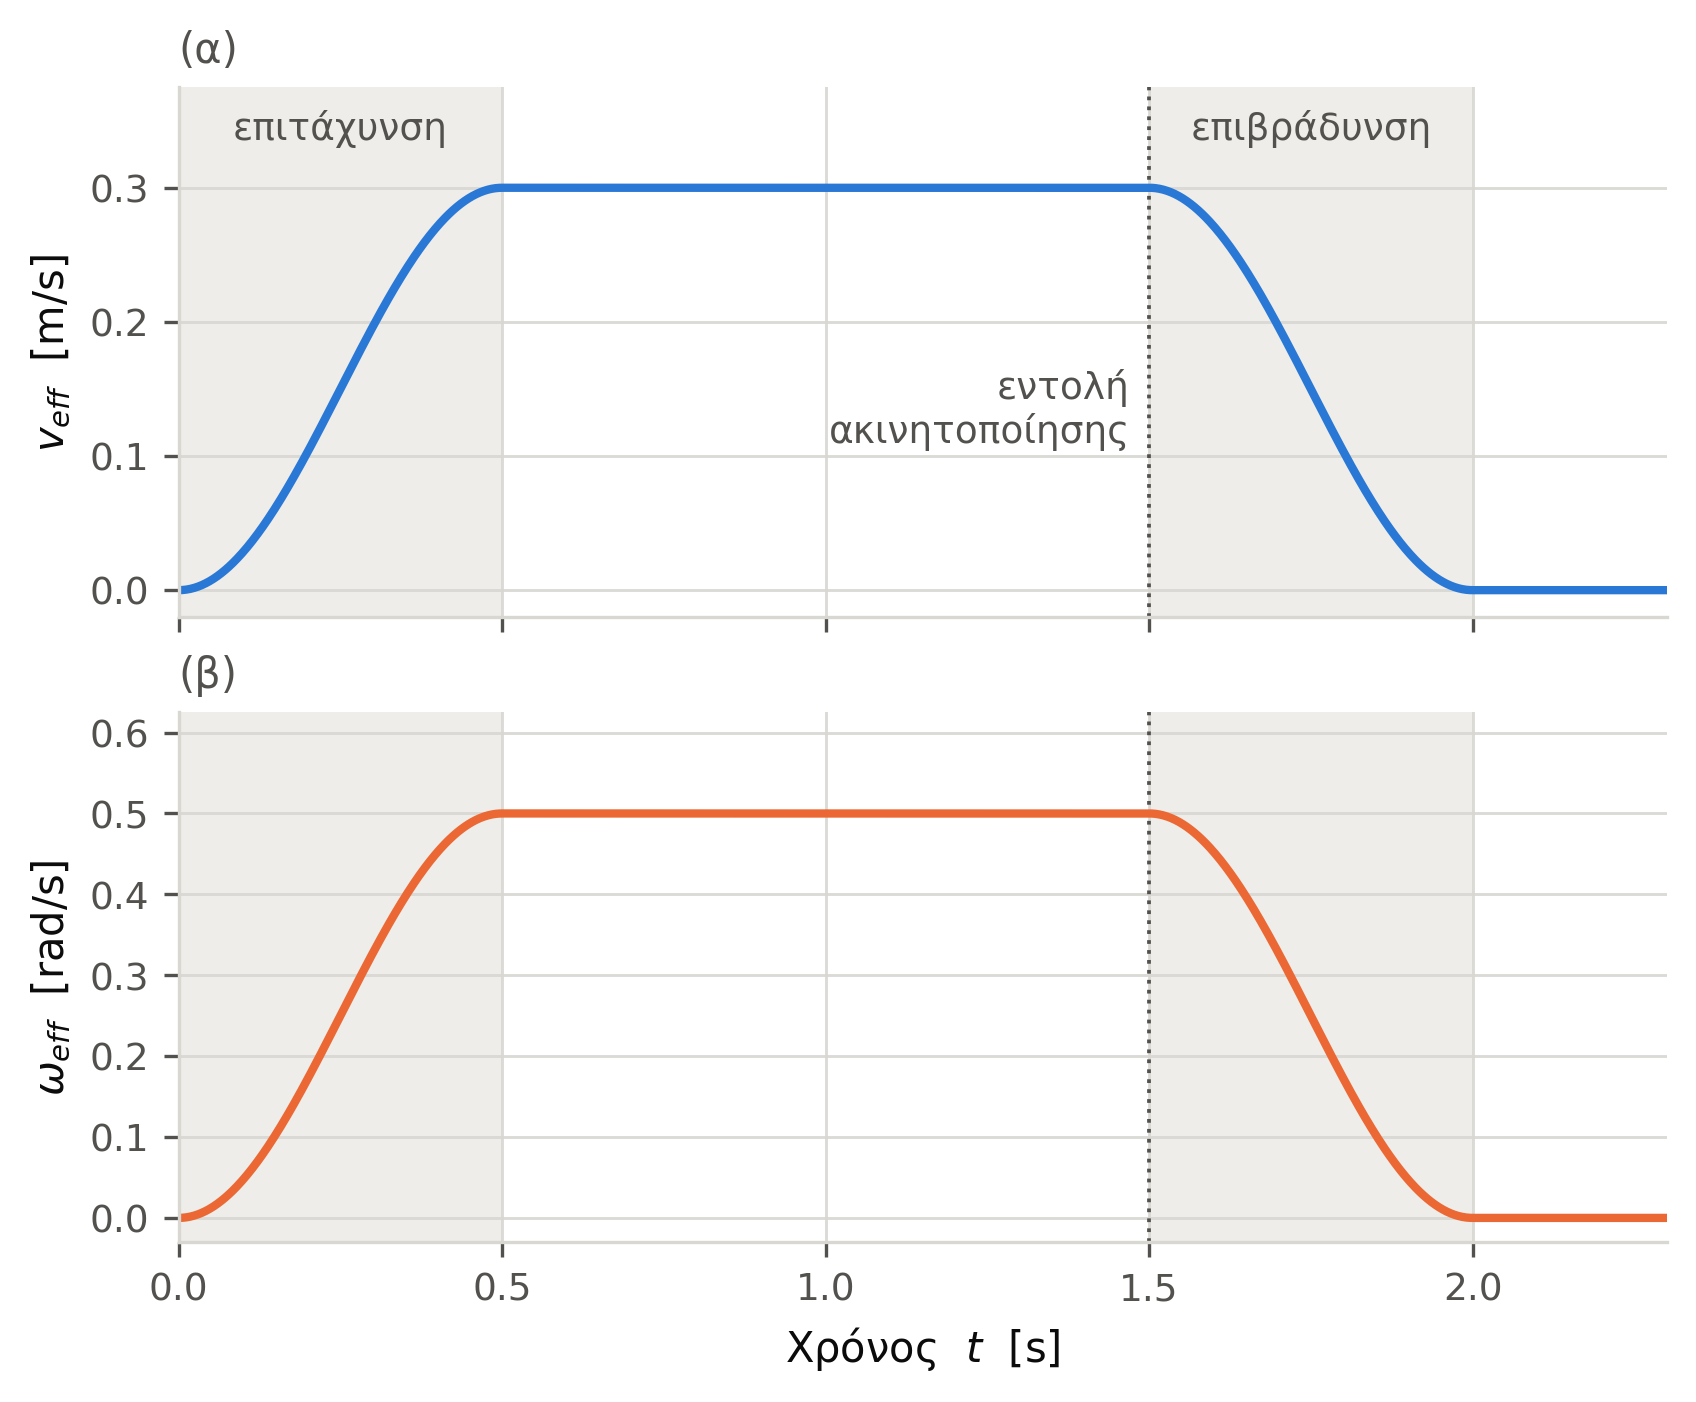
\includegraphics[width=0.92\textwidth]{images/velocity_ramp.png}
    \caption[Συνημιτονοειδής ράμπα ταχύτητας]{Εφαρμογή της συνημιτονοειδούς
    ράμπας με $T_r = 0{,}5$~s στη γραμμική και στη γωνιακή ταχύτητα, κατά την
    εκκίνηση και μετά την εντολή ακινητοποίησης. Οι τιμές $v = 0{,}3$~m/s και
    $\omega = 0{,}5$~rad/s είναι ενδεικτικές}
    \label{fig:velocity-ramp}
\end{figure}

\section{Σχεδιασμός Βαδίσματος Στροφής}
\label{sec:turning-gait}
Αφετηρία για τον σχεδιασμό της βάδισης στροφής είναι ο τρόπος με τον οποίο
στρίβει ένα όχημα με διαφορικό σύστημα (differential system): κάθε τροχός
λαμβάνει διαφορετική ταχύτητα ή κατεύθυνση, και ανάλογα με τον συνδυασμό τους το
όχημα στρίβει είτε επί τόπου είτε εν κινήσει \cite{lee_turning_2014}. Για να
μεταφερθεί η λογική αυτή σε τετράποδο, πρέπει πρώτα κάθε πόδι να μπορεί να
κινηθεί προς οποιαδήποτε κατεύθυνση του οριζόντιου επιπέδου και όχι μόνο κατά
μήκος των βασικών αξόνων.

Για τον σκοπό αυτό εισάγεται η γωνία πλευρικής κατεύθυνσης (lateral fraction)
$\lambda$, όπως στη γεννήτρια βαδίσματος του SpotMiniMini
\cite{spotminimini2020github}. Η γωνία μετράται από τον άξονα $X$ προς τον άξονα
$Z$, με $\lambda = 0$ για κίνηση εμπρός, $\lambda = \pi$ πίσω και
$\lambda = \pm\pi/2$ πλάγια. Η μετατόπιση $d$ των \eqref{eq:swing-offset} και
\eqref{eq:stance-x} προβάλλεται στους δύο οριζόντιους άξονες, ενώ η κατακόρυφη
συνιστώσα $h$ μένει αμετάβλητη:
\begin{equation}
\mathbf{p}(t) = \mathbf{p}^0 + \left(d\cos\lambda,\ h,\ d\sin\lambda\right),
\label{eq:omni-foot}
\end{equation}
όπου $\mathbf{p}^0$ η ονομαστική θέση του πέλματος. Ισοδύναμα, σε κάθε πόδι
αντιστοιχίζεται το διάνυσμα βήματος $S\,(\cos\lambda,\ \sin\lambda)$, με
$S = v_{eff}\,T_{cyc}\,\beta$, και το κατακόρυφο επίπεδο της τροχιάς στρέφεται
κατά $\lambda$ περί τον κατακόρυφο άξονα. Όταν όλα τα πόδια έχουν το ίδιο
διάνυσμα, το σώμα μετατοπίζεται προς την κατεύθυνση $\lambda$ χωρίς να
περιστρέφεται.

Με τη βάση αυτή, η περιστροφή προκύπτει δίνοντας σε κάθε πόδι διαφορετικό
διάνυσμα βήματος, όπως στους τροχούς του διαφορικού συστήματος. Το
\cite{lee_turning_2014} συνδυάζει το διαφορικό σύστημα, μεταβάλλοντας κατά ίσες
και αντίθετες ποσότητες το μήκος διασκελισμού των εξωτερικών και των εσωτερικών
ποδιών, εξισώσεις (5) έως (7), με ένα σύστημα διεύθυνσης τύπου 4WS, στρέφοντας
την τροχιά κάθε ποδιού περί τον κατακόρυφο άξονα, εξίσωση (4). Με παρόμοιο
τρόπο, το \cite{liu_turning_2017} υπολογίζει γεωμετρικά από την ακτίνα στροφής
διαφορετικό μήκος βήματος για το εσωτερικό και το εξωτερικό πόδι και στρέφει
ανάλογα την τροχιά τους, εξισώσεις (1) έως (6).

Στην υλοποίηση ακολουθείται η απλούστερη προσέγγιση του SpotMiniMini
\cite{spotminimini2020github}, όπου η γωνιακή ταχύτητα $\omega$ προσθέτει σε κάθε
πόδι ένα δεύτερο διάνυσμα βήματος. Αν $\rho_i$ και $\gamma_i$ είναι οι πολικές
συντεταγμένες της ονομαστικής θέσης του πέλματος στο οριζόντιο επίπεδο, το μέτρο
και η διεύθυνση του διανύσματος αυτού είναι
\begin{equation}
S_{\omega,i} = \omega_{eff}\,T_{cyc}\,\rho_i, \qquad
\chi_i =
\begin{cases}
\pi/2 + \gamma_i + \varepsilon_i, & i \in \{FR,\ RL\} \\
\pi/2 - \gamma_i + \varepsilon_i, & i \in \{FL,\ RR\},
\end{cases}
\label{eq:yaw-step}
\end{equation}
με $\varepsilon_i = \operatorname{atan2}(g_i,\ \rho_i)$ μια μικρή διόρθωση, όπου
$g_i$ η απόσταση του πέλματος στο προηγούμενο βήμα ελέγχου από την ονομαστική
του θέση. Τα δύο διανύσματα αθροίζονται ανά πόδι,
\begin{equation}
s_{x,i} = S\cos\lambda + S_{\omega,i}\cos\chi_i, \qquad
s_{z,i} = S\sin\lambda + S_{\omega,i}\sin\chi_i,
\label{eq:step-sum}
\end{equation}
και το μέτρο $S_i = \sqrt{s_{x,i}^2 + s_{z,i}^2}$ και η γωνία
$\lambda_i = \operatorname{atan2}(s_{z,i},\ s_{x,i})$ του αθροίσματος
αντικαθιστούν τα $S$ και $\lambda$ της \eqref{eq:omni-foot}
(Σχήμα~\ref{fig:turning-geometry}). Με $v = 0$ το
ρομπότ στρέφεται επί τόπου, ενώ με $v \neq 0$ στρίβει εν κινήσει, με ακτίνα
στροφής που καθορίζεται από τον λόγο $v/\omega$.


Τέλος, κατά τη στροφή εν κινήσει η κεντρομόλος επιτάχυνση τείνει να ανατρέψει
το σώμα προς το εξωτερικό της στροφής. Όπως στο \cite{lee_turning_2014},
εξίσωση (10), υπολογίζεται η γωνία κλίσης σώματος (banked roll)
\begin{equation}
\theta_b = \operatorname{sgn}(\omega_{eff})\,
\tan^{-1}\!\left(\frac{v_{eff}^2}{g\,R}\right), \qquad
R = \frac{|v_{eff}|}{|\omega_{eff}|},
\label{eq:banked-roll}
\end{equation}
η οποία προστίθεται στη μετρούμενη γωνία roll πριν από τον ελεγκτή
σταθεροποίησης (ενότητα~\ref{sec:stabilization}), ώστε το σώμα να γέρνει κατά
τη στροφή αντί να διατηρείται οριζόντιο.

\begin{figure}[htbp]
    \centering
    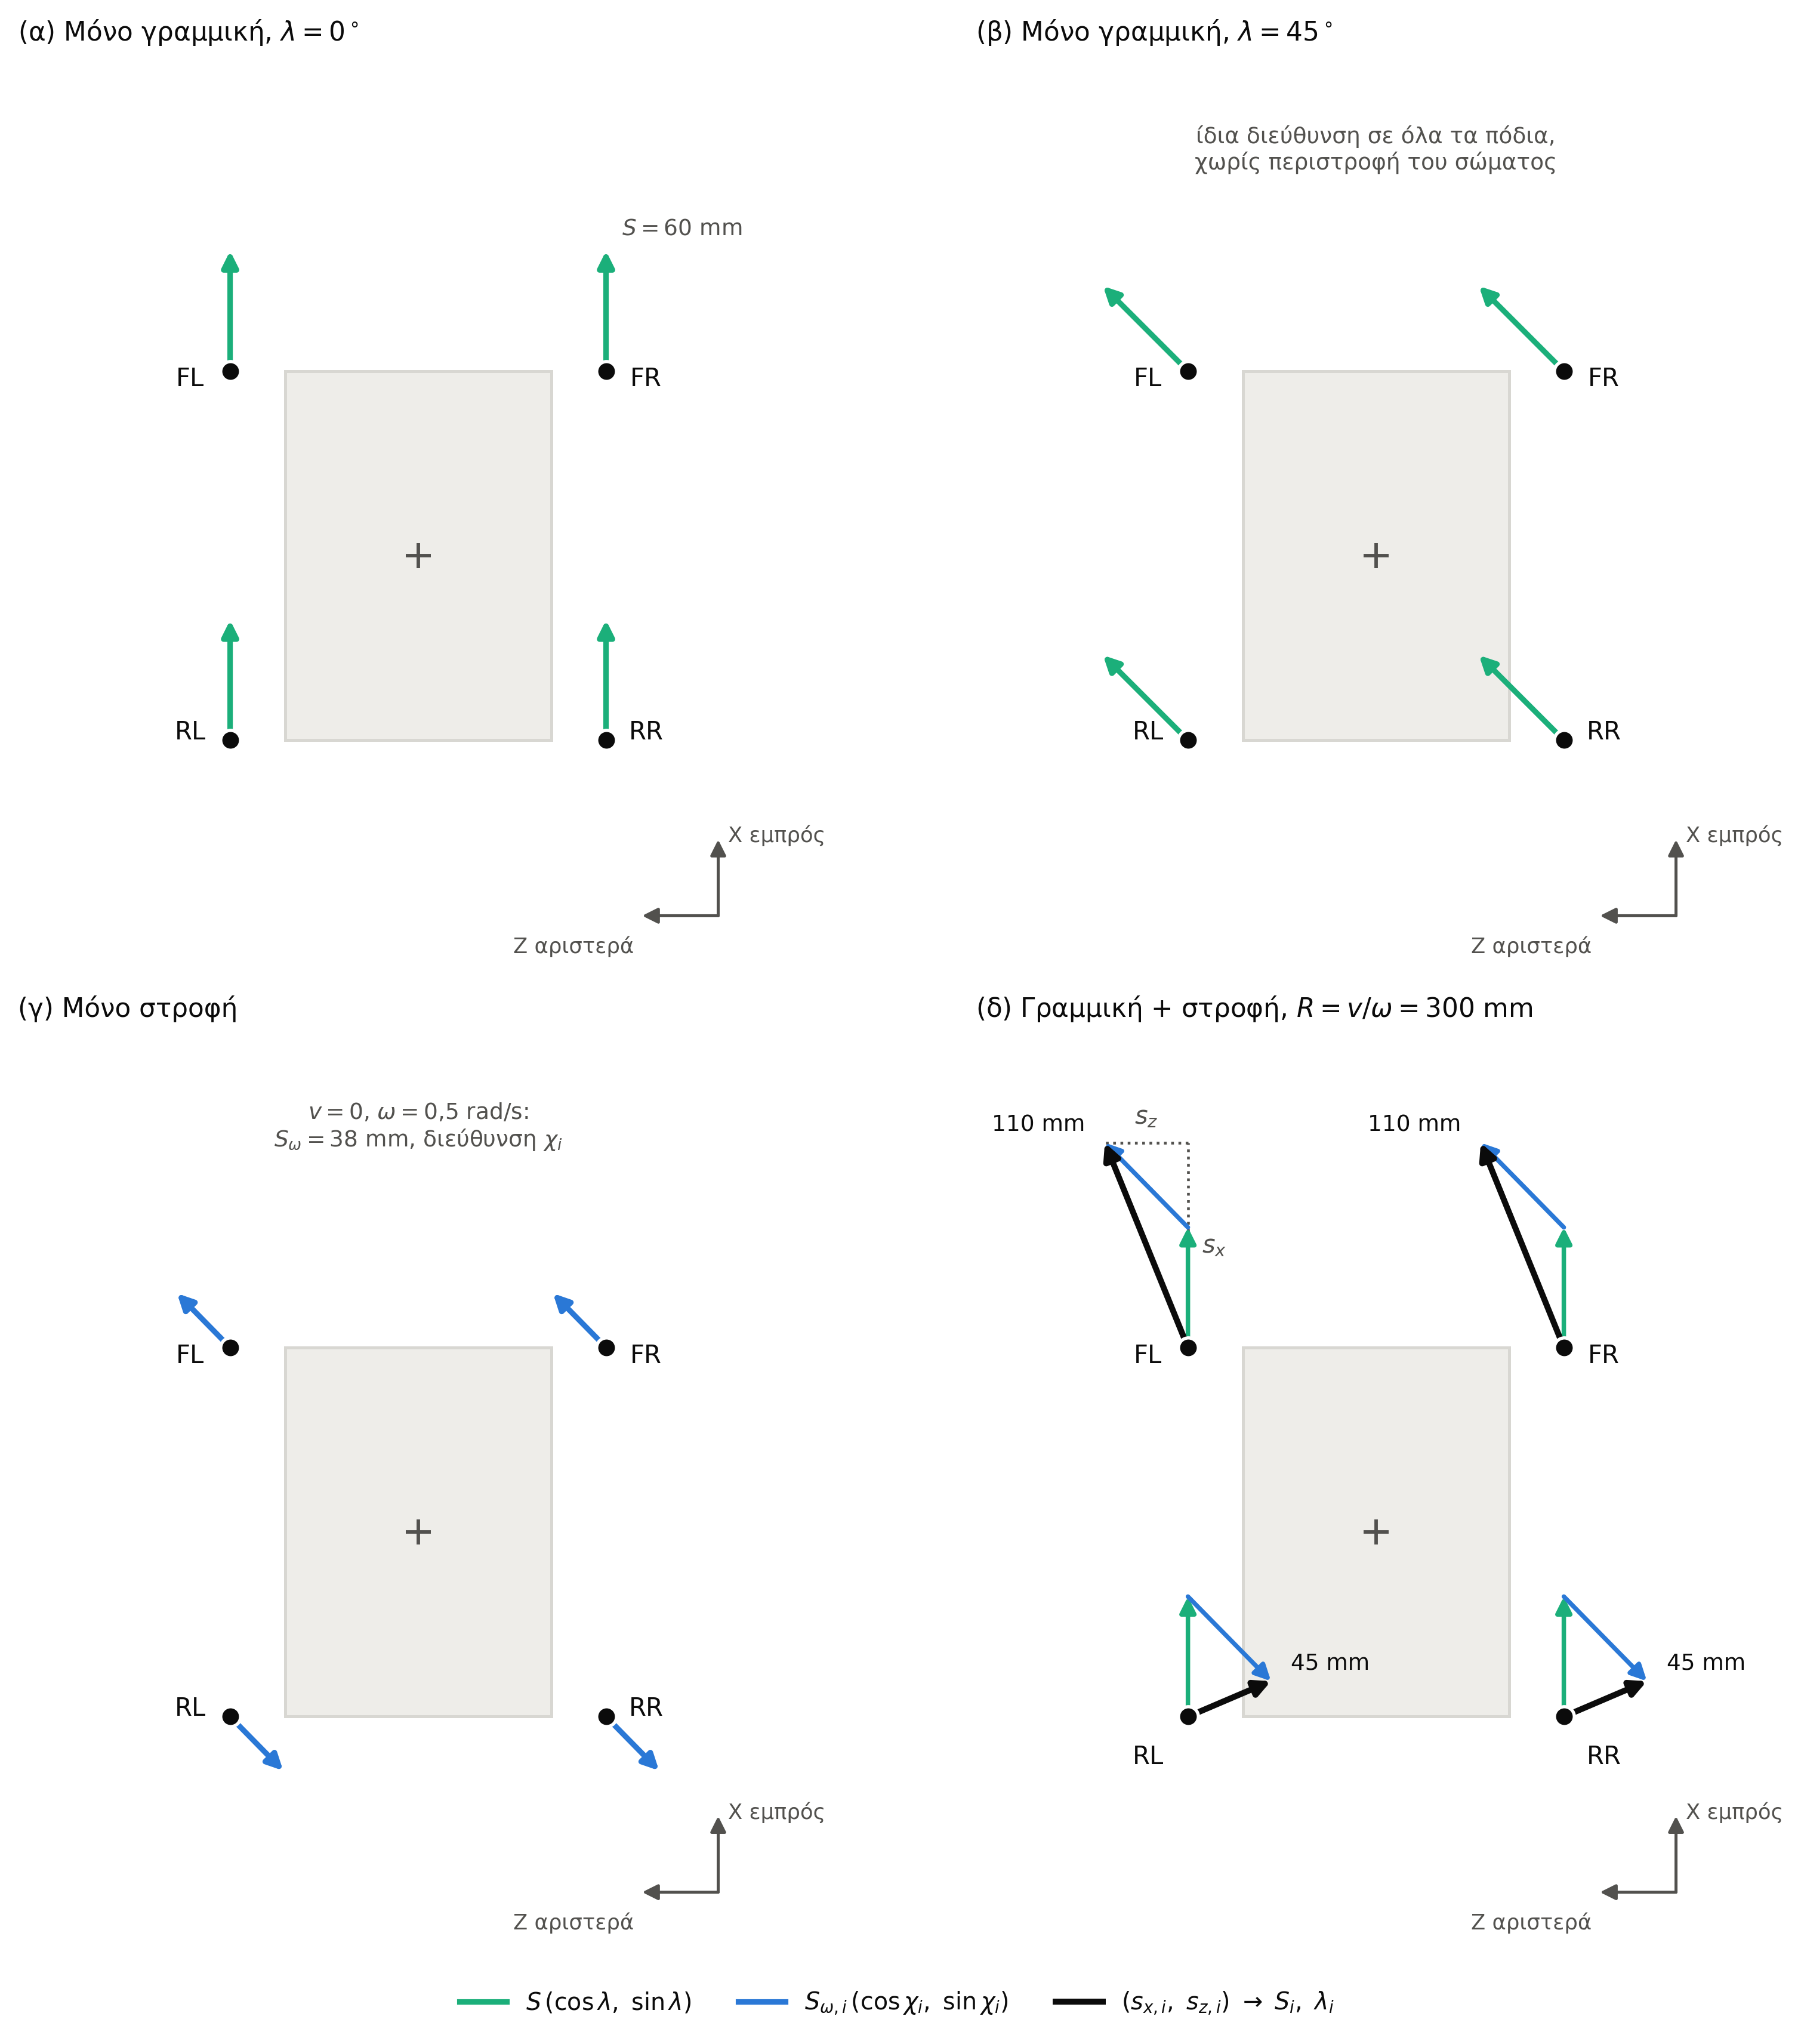
\includegraphics[width=0.85\textwidth]{images/step_composition.png}
    \caption[Σύνθεση του διανύσματος βήματος ανά πόδι]{Διάνυσμα βήματος ανά
    πόδι: (α) κίνηση εμπρός, (β) κίνηση υπό γωνία $\lambda = 45^\circ$, (γ)
    στροφή επί τόπου, (δ) στροφή εν κινήσει με $R = v/\omega = 300$~mm}
    \label{fig:turning-geometry}
\end{figure}

\section{Σταθεροποίηση Προσανατολισμού}
\label{sec:stabilization}
Παρόλο που το ρομπότ σχεδιάστηκε για κίνηση σε επίπεδο δάπεδο, κατασκευαστικές
ατέλειες και η εγγενής μη γραμμικότητα του συστήματος προκαλούν αστάθεια κατά
την κίνηση: το σώμα γέρνει και σε ορισμένες περιπτώσεις το ρομπότ πέφτει προς τα
εμπρός. Για τον λόγο αυτό υλοποιήθηκε ελεγκτής που διατηρεί το σώμα οριζόντιο. Η
δομή του είναι απλή: ένας ελεγκτής PID δρα στις γωνίες roll και pitch, και η
έξοδός του μετατρέπεται γεωμετρικά σε κατακόρυφη μετατόπιση κάθε πέλματος, η
οποία εφαρμόζεται μέσω της αντίστροφης κινηματικής
(Σχήμα~\ref{fig:control-loop-block}).

\begin{figure}[htbp]
    \centering
    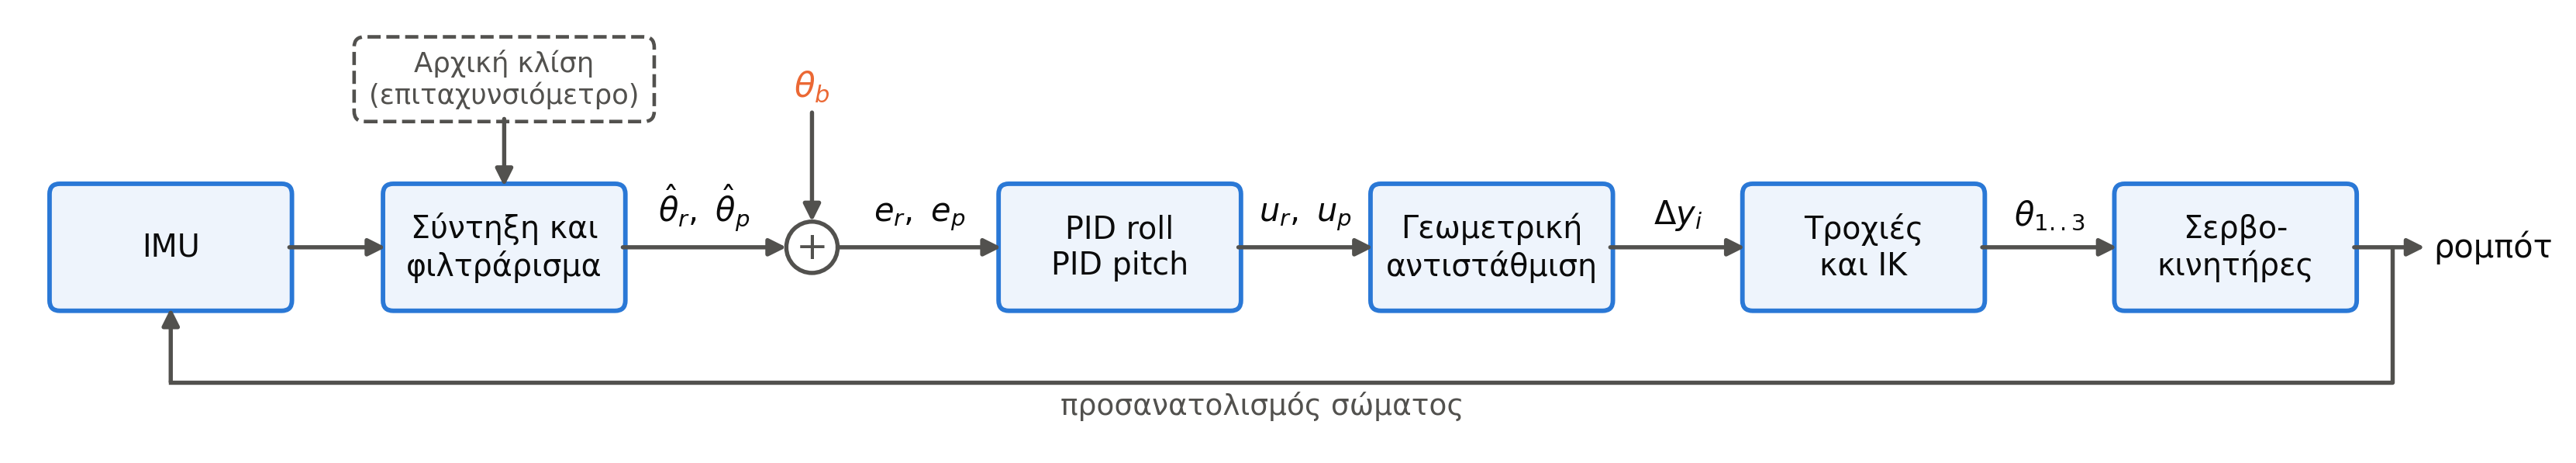
\includegraphics[width=\textwidth]{images/control_loop.png}
    \caption[Βρόχος ελέγχου σταθεροποίησης]{Βρόχος ελέγχου σταθεροποίησης
    προσανατολισμού}
    \label{fig:control-loop-block}
\end{figure}

Οι γωνίες $\hat{\theta}_r$ (roll) και $\hat{\theta}_p$ (pitch) εκτιμώνται από το
IMU μέσω σύντηξης αισθητήρων και φιλτραρίσματος. Κατά την εκκίνηση, με το ρομπότ
ακίνητο, το επιταχυνσιόμετρο μετρά μόνο τη βαρύτητα, οπότε η αρχική κλίση
υπολογίζεται απευθείας από τις συνιστώσες $a_x$, $a_y$, $a_z$ της μέτρησης,
εξισώσεις (25) και (26) του \cite{pedley_tilt_2013}:
\begin{equation}
\theta_{r,0} = \operatorname{atan2}\!\left(a_y,\ a_z\right), \qquad
\theta_{p,0} = \operatorname{atan2}\!\left(-a_x,\ \sqrt{a_y^2 + a_z^2}\right).
\label{eq:tilt-acc}
\end{equation}
Η εκτίμηση αυτή χρησιμοποιείται ως αρχική τιμή του φίλτρου σύντηξης και
αφαιρείται από τις επόμενες μετρήσεις, ώστε ο ελεγκτής να ξεκινά από ένα γνωστό
σημείο αναφοράς και όχι από αυθαίρετη αρχική τιμή.

\subsection{Ελεγκτής PID Roll/Pitch}
Για κάθε γωνία $j \in \{r,\ p\}$ χρησιμοποιείται ανεξάρτητος ελεγκτής PID. Η
επιθυμητή κλίση είναι μηδενική, οπότε σφάλμα είναι η ίδια η μετρούμενη γωνία,
με την προσθήκη της γωνίας $\theta_b$ της \eqref{eq:banked-roll} στο roll:
\begin{equation}
e_r = \hat{\theta}_r + \theta_b, \qquad e_p = \hat{\theta}_p.
\label{eq:pid-error}
\end{equation}
Η έξοδος στο βήμα ελέγχου $k$ είναι
\begin{equation}
u_j[k] = K_p\,e_j[k] + K_i\,I_j[k] + K_d\,\frac{e_j[k] - e_j[k-1]}{\Delta t_k},
\qquad
I_j[k] = \operatorname{sat}\!\left(I_j[k-1] + e_j[k]\,\Delta t_k\right),
\label{eq:pid-output}
\end{equation}
όπου η $\operatorname{sat}$ περιορίζει τον ολοκληρωτικό όρο στο
$[-I_{max},\ I_{max}]$ ως μέτρο anti-windup \cite{caparroz_antiwindup_2026}. Οι
τιμές των κερδών δίνονται στον Πίνακα~\ref{tab:pid-gains}.

\begin{table}[htbp]
    \centering
    \small
    \begin{tabular}{@{}l l l@{}}
        \toprule
        Παράμετρος & Σύμβολο & Τιμή \\
        \midrule
        Αναλογικό κέρδος & $K_p$ & $0{,}4$ \\
        Ολοκληρωτικό κέρδος & $K_i$ & $0{,}025$ \\
        Διαφορικό κέρδος & $K_d$ & $0{,}05$ \\
        Όριο ολοκληρωτικού όρου & $I_{max}$ & $0{,}7$ \\
        \bottomrule
    \end{tabular}
    \caption[Κέρδη των ελεγκτών PID]{Κέρδη των ελεγκτών PID, κοινά για roll και
    pitch}
    \label{tab:pid-gains}
\end{table}

\subsection{Γεωμετρική Αντιστάθμιση Ύψους Άκρων}
Αρχικά ο ελεγκτής διόρθωνε απευθείας τη στάση του σώματος μέσω του
μετασχηματισμού σώματος της ενότητας~\ref{subsec:body-transform}. Στη βιβλιογραφία
όμως η απόκλιση που μετρά το IMU μετατρέπεται σε μετατόπιση ύψους των άκρων, και
ο ελεγκτής δρα πάνω σε αυτή τη μετατόπιση
\cite{mori_study_2022,prayogo_quadruped_2018}. Στην παρούσα εργασία ο ελεγκτής
διορθώνει τις γωνίες roll και pitch, και η διόρθωση μεταφέρεται έπειτα
γεωμετρικά στα άκρα. Κλίση κατά γωνία $u$ μετατοπίζει ένα σημείο σε απόσταση
$W/2$ από τον άξονα περιστροφής κατά $(W/2)\tan u$
(Σχήμα~\ref{fig:foot-height-compensation}), οπότε η διόρθωση κάθε ποδιού είναι
\begin{equation}
\begin{aligned}
\Delta y_{FL} &= +\tfrac{W}{2}\tan u_r + \tfrac{L}{4}\tan u_p, \\
\Delta y_{FR} &= -\tfrac{W}{2}\tan u_r + \tfrac{L}{4}\tan u_p, \\
\Delta y_{RL} &= +\tfrac{W}{2}\tan u_r - \tfrac{L}{4}\tan u_p, \\
\Delta y_{RR} &= -\tfrac{W}{2}\tan u_r - \tfrac{L}{4}\tan u_p,
\end{aligned}
\label{eq:foot-height-comp}
\end{equation}
με τον συντελεστή $L/4$ όπως στην εξίσωση (4) του \cite{mori_study_2022}. Η
$\Delta y_i$ προστίθεται στην κατακόρυφη συντεταγμένη της ονομαστικής θέσης του
πέλματος, οπότε μεταφέρεται και στις δύο φάσεις της τροχιάς, και οι γωνίες των
αρθρώσεων προκύπτουν από την αντίστροφη κινηματική.

\begin{figure}[htbp]
    \centering
    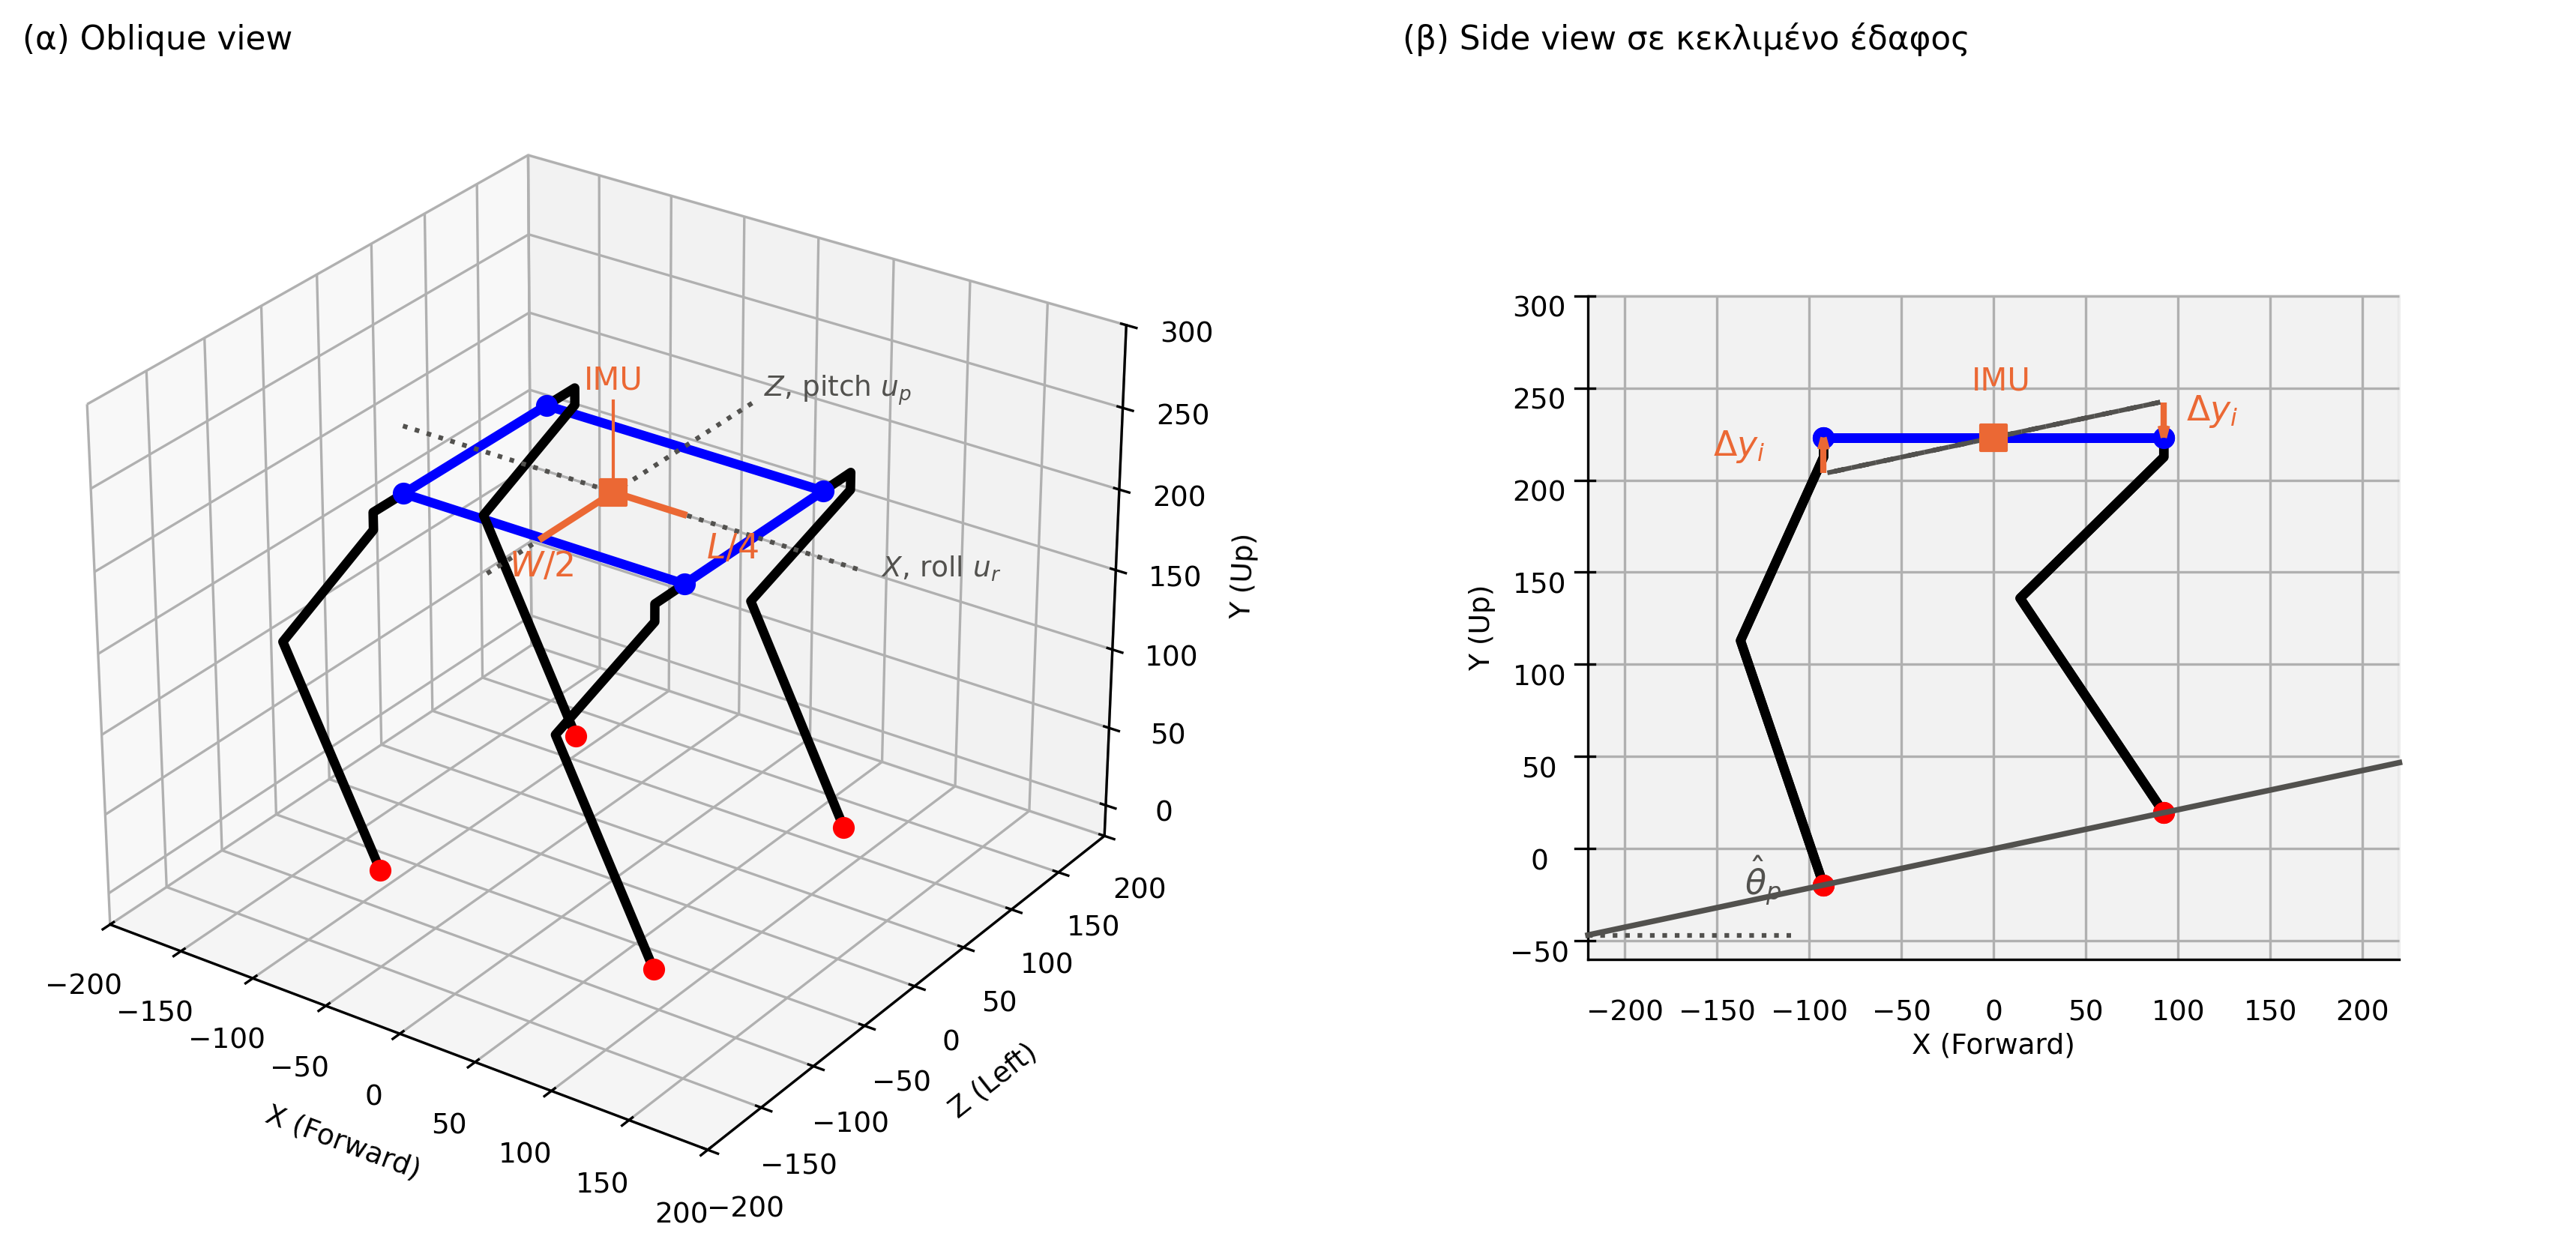
\includegraphics[width=0.95\textwidth]{images/foot_height_compensation.png}
    \caption[Γεωμετρική αντιστάθμιση ύψους άκρων]{(α) Θέση του IMU και
    αποστάσεις $W/2$ και $L/4$ της \eqref{eq:foot-height-comp}. (β) Πλάγια όψη
    σε κεκλιμένο έδαφος: με τη διόρθωση $\Delta y_i$ το σώμα παραμένει
    οριζόντιο, ενώ με διακεκομμένη γραμμή φαίνεται το σώμα χωρίς αντιστάθμιση.
    Κατά το πρότυπο του Σχήματος 4 του \cite{mori_study_2022}}
    \label{fig:foot-height-compensation}
\end{figure}

% --- Simulation ---
\chapter{Προσομοίωση}
\textit{[προς συμπλήρωση]}

\section{Επιλογή Περιβάλλοντος Προσομοίωσης}
\textit{[προς συμπλήρωση]}

\tabTODO{Σύγκριση περιβαλλόντων προσομοίωσης (PyBullet, Gazebo, Webots,
MuJoCo) και κριτήρια επιλογής}{tab:sim-env-comparison}

\section{Μοντέλο Ρομπότ και Αντιστοίχιση Αξόνων}
\textit{[προς συμπλήρωση]}

\figTODO{Το μοντέλο URDF του ρομπότ στο PyBullet, με διάγραμμα αντιστοίχισης
αξόνων PyBullet$\leftrightarrow$ρομπότ}{fig:pybullet-urdf-screenshot}

\section{Υλοποίηση Βρόχου Ελέγχου}
\textit{[προς συμπλήρωση]}

\figTODO{Flowchart του βρόχου ελέγχου στην προσομοίωση}{fig:sim-control-loop}

\section{Ρύθμιση Παραμέτρων Ελεγκτή}
\textit{[προς συμπλήρωση]}

\figTODO{Βηματική απόκριση για διαφορετικά κέρδη PID κατά τη ρύθμιση
παραμέτρων}{fig:sim-tuning-response}

\tabTODO{Τελικές ρυθμισμένες παράμετροι ελεγκτή από την
προσομοίωση}{tab:sim-tuned-params}

% --- Real Hardware Implementation ---
\chapter{Υλοποίηση σε Πραγματικό Ρομπότ}
\label{ch:hardware}
\textit{[προς συμπλήρωση]}

\section{Σχεδιασμός και Εκτύπωση Σκελετού Ρομπότ}
\textit{[προς συμπλήρωση]}

\figTODO{CAD renders και φωτογραφίες των τρισδιάστατα τυπωμένων
μερών ΑΠΟ ΚΟΝΤΑ}{fig:skeleton-cad-photos}

\section{Hardware}
\textit{[προς συμπλήρωση]}

\figTODO{Φωτογραφία/block diagram της πλήρους στοίβας υλικού: Raspberry Pi 5,
2$\times$PCA9685, μπαταρία, IMU ΑΠΟ ΚΟΝΤΑ}{fig:hardware-stack-photo}

\tabTODO{Κατάλογος υλικών (BOM): εξάρτημα, προδιαγραφές και κόστος}{tab:bom}

\subsection{Επιλογή Κινητήρων}
\textit{[προς συμπλήρωση]}

\figTODO{Σερβοκινητήρας Feetech FT5116M ΑΠΟ ΚΟΝΤΑ}{fig:servo-photo}

\tabTODO{Προδιαγραφές σερβοκινητήρα Feetech FT5116M (ροπή, ταχύτητα,
τάση λειτουργίας)}{tab:servo-specs}

\subsection{Επιλογή Υπολογιστικής Μονάδας}
\textit{[προς συμπλήρωση]}

\figTODO{Raspberry Pi 5 ΑΠΟ ΚΟΝΤΑ}{fig:rpi5-photo}

\subsection{Επιλογή Αισθητήρων}
\textit{[προς συμπλήρωση]}

\figTODO{Αδρανειακή μονάδα GY-85 (ADXL345 + ITG-3200 + QMC5883L) ΑΠΟ ΚΟΝΤΑ}{fig:imu-photo}

\subsection{Τροφοδοσία και Επιμέρους Ηλεκτρονικά}
\textit{[προς συμπλήρωση]}

\figTODO{Διάγραμμα καλωδίωσης ισχύος: μπαταρία $\rightarrow$
2$\times$XL4015 step-down $\rightarrow$ PCA9685, τροφοδοσία Raspberry Pi 5
5V/5A ΑΠΟ ΚΟΝΤΑ}{fig:power-wiring-diagram}

\section{Αρχιτεκτονική Λογισμικού}
\label{sec:software-architecture}
\textit{[προς συμπλήρωση]}

\figTODO{Block diagram αρχιτεκτονικής λογισμικού (core/, hw/, sim/,
tools/)}{fig:software-architecture}

\section{Οδήγηση και Βαθμονόμηση Σερβοκινητήρων}
\textit{[προς συμπλήρωση]}

\figTODO{Γωνία σερβοκινητήρα συναρτήσει πλάτους παλμού
(PWM) ΜΕΤΡΗΣΗ ΣΤΟ ΡΟΜΠΟΤ}{fig:servo-calibration-plot}

\tabTODO{Offset βαθμονόμησης ανά σερβοκινητήρα (12 τιμές), όπως
αποθηκεύονται στο \texttt{servo\_calib.yaml}}{tab:servo-calib-offsets}

\section{Sensors Fusion}
\label{sec:sensor-fusion}
\textit{[προς συμπλήρωση \cite{garcia_ahrs,cocoli_comparative_2023}]}

\subsection{Φίλτρο Kalman}
\textit{[προς συμπλήρωση \cite{palanisamy_filtering_2016,kalman_new_1960,
sabatini_kalmanfilterbased_2011,garcia_ahrs}]}

\figTODO{Block diagram του φίλτρου Kalman}{fig:kalman-block}

\subsection{Φίλτρο Madgwick}
\textit{[προς συμπλήρωση \cite{madgwick_efficient_2010,garcia_ahrs}]}

\figTODO{Block diagram του φίλτρου Madgwick}{fig:madgwick-block}

\subsection{Βαθμονόμηση και Θόρυβος Αισθητήρων}
\textit{[προς συμπλήρωση]}

\figTODO{Ακατέργαστο (raw) έναντι φιλτραρισμένου σήματος
αισθητήρα ΜΕΤΡΗΣΗ ΣΤΟ ΡΟΜΠΟΤ}{fig:sensor-noise-plot}

\tabTODO{Σύγκριση φίλτρων Kalman και Madgwick: υπολογιστικό κόστος,
ακρίβεια, πολυπλοκότητα υλοποίησης}{tab:filter-comparison}

\section{Έλεγχος σε Πραγματικό Χρόνο}
\textit{[προς συμπλήρωση]}

\subsection{Φιλτράρισμα Σήματος (30-tap Moving Average)}
\textit{[προς συμπλήρωση]}

\figTODO{Σήμα roll/pitch πριν και μετά το 30-tap φιλτράρισμα κινούμενου
μέσου ΜΕΤΡΗΣΗ ΣΤΟ ΡΟΜΠΟΤ}{fig:moving-average-plot}

\subsection{Υλοποίηση Ελεγκτή PID}
\textit{[προς συμπλήρωση]}

\figTODO{Απόκριση roll/pitch του ελεγκτή PID σε πραγματικό
χρόνο ΜΕΤΡΗΣΗ ΣΤΟ ΡΟΜΠΟΤ}{fig:pid-realtime-response}

\section{Τηλεχειρισμός}
\textit{[προς συμπλήρωση]}

\figTODO{Χειριστήριο DualSense και αντιστοίχιση εντολών
τηλεχειρισμού ΑΠΟ ΚΟΝΤΑ}{fig:teleop-photo}

\section{Καταγραφή Δεδομένων}
\textit{[προς συμπλήρωση]}

\figTODO{Δείγμα γραφήματος καταγεγραμμένων δεδομένων
(\texttt{log\_plotter.py}) ΜΕΤΡΗΣΗ ΣΤΟ ΡΟΜΠΟΤ}{fig:log-plotter-sample}

% --- Results ---
\chapter{Αποτελέσματα}
\textit{[προς συμπλήρωση]}

\section{Μεθοδολογία Πειραμάτων}
\textit{[προς συμπλήρωση]}

\tabTODO{Πειραματικός σχεδιασμός: μετρούμενα μεγέθη, αριθμός επαναλήψεων
και συνθήκες δοκιμής}{tab:experiment-design}

\section{Αποτελέσματα Προσομοίωσης}
\textit{[προς συμπλήρωση]}

\figTODO{Γραφήματα τροχιάς και roll/pitch από την προσομοίωση}{fig:sim-results-plots}

\section{Αποτελέσματα Βάδισης σε Πραγματικό Ρομπότ}
\textit{[προς συμπλήρωση]}

\figTODO{Ακολουθία καρέ βάδισης trot και στροφής, με ποσοτικά γραφήματα
ταχύτητας και roll/pitch ΑΠΟ ΚΟΝΤΑ ΚΑΙ ΜΕΤΡΗΣΗ ΣΤΟ ΡΟΜΠΟΤ}{fig:real-robot-gait-frames}

\tabTODO{Μετρικές απόδοσης βάδισης ανά δοκιμή: ταχύτητα, RMS σφάλμα
roll/pitch ΜΕΤΡΗΣΗ ΣΤΟ ΡΟΜΠΟΤ}{tab:gait-performance-metrics}

\section{Απόκριση Ελεγκτή Σταθεροποίησης}
\textit{[προς συμπλήρωση]}

\figTODO{Σύγκριση απόκρισης με και χωρίς σταθεροποίηση, και απόκριση σε
διαταραχή ΜΕΤΡΗΣΗ ΣΤΟ ΡΟΜΠΟΤ}{fig:controller-response-comparison}

\tabTODO{Σύγκριση μετρικών απόδοσης με και χωρίς
σταθεροποίηση ΜΕΤΡΗΣΗ ΣΤΟ ΡΟΜΠΟΤ}{tab:stabilization-comparison}

\section{Βίντεο}
\textit{[προς συμπλήρωση — σύνδεσμοι/αναφορές σε επίδειξη λειτουργίας]}

\figTODO{QR code / frame grabs με σύνδεσμο προς το βίντεο
επίδειξης ΒΙΝΤΕΟ ΣΤΟ ΡΟΜΠΟΤ}{fig:video-qr}

% --- Conclusions ---
\chapter{Συμπεράσματα και Μελλοντικές Επεκτάσεις}
\textit{[προς συμπλήρωση]}

\section{Σύνοψη Εργασίας}
\textit{[προς συμπλήρωση]}

\section{Περιορισμοί}
\textit{[προς συμπλήρωση]}

\section{Μελλοντικές Επεκτάσεις}
\label{sec:future-work}
\textit{[προς συμπλήρωση]}

% --- Appendices ---
\appendix
\addcontentsline{toc}{chapter}{Παραρτήματα}

\chapter{Φυσικές Διαστάσεις και Παράμετροι Ρομπότ}
\textit{[προς συμπλήρωση]}

\figTODO{Διαστασιολογημένο σχέδιο του ρομπότ (μήκη σκελών, πλάτος/μήκος
σώματος) από το \texttt{robot\_config.yaml} ΜΕΤΡΗΣΗ ΣΤΟ ΡΟΜΠΟΤ ΓΙΑ
ΕΠΑΛΗΘΕΥΣΗ}{fig:robot-dimensions-drawing}

\tabTODO{Πλήρης πίνακας φυσικών διαστάσεων (mm) και ορίων άρθρωσης, όπως
ορίζονται στο \texttt{robot\_config.yaml}}{tab:appendix-dimensions}

\chapter{Παράμετροι Ελεγκτή και Βάδισης}
\textit{[προς συμπλήρωση]}

\tabTODO{Πλήρης πίνακας παραμέτρων βάδισης (Tswing, Tstance, βάθος
διείσδυσης δ, σημεία ελέγχου Bezier)}{tab:appendix-gait-params}

\tabTODO{Πλήρης πίνακας παραμέτρων ελεγκτή σταθεροποίησης (κέρδη PID,
συντελεστές γεωμετρικής αντιστάθμισης)}{tab:appendix-controller-params}

% --- Bibliography ---
\clearpage
\addcontentsline{toc}{chapter}{Βιβλιογραφία}
\printbibliography[title={Βιβλιογραφία}]

\end{document}
